\documentclass[specialist,
substylefile = spbu.rtx,
               subf,href,colorlinks=true, 12pt]{disser}
\usepackage[a4paper,
            mag=1000, includefoot,
            left=3cm, right=1.5cm, top=2cm, bottom=2cm, headsep=1cm, footskip=1cm]{geometry}
\usepackage[T2A]{fontenc}
%\usepackage[cp1251]{inputenc}
\usepackage[utf8]{inputenc}
\usepackage[english,russian]{babel}

\righthyphenmin=2
\usepackage{indentfirst}
\usepackage{amsmath}
\usepackage{multirow}
\usepackage{array}
\usepackage{booktabs}
\usepackage{pdflscape}
\usepackage{amssymb}
\usepackage{ dsfont }
\usepackage[table]{xcolor}
\usepackage{graphicx}
\usepackage{vmargin}
\usepackage{wrapfig}

\usepackage{booktabs} % Для красивых линий
\usepackage{siunitx} % Для форматирования чисел
\usepackage{caption} % Для настройки подписей

\usepackage{longtable}
\usepackage{footnote}
\usepackage{breqn}
\renewcommand{\baselinestretch}{1.5}
\usepackage{amsfonts}
\usepackage{listings}
\usepackage{subcaption}
\DeclareMathOperator{\spdepth}{spdepth}
\DeclareMathOperator{\odepth}{odepth}
\DeclareMathOperator{\sign}{sign}

\newcommand{\rmT}{\mathrm{T}}

\usepackage{amsthm}
\usepackage{mathtools}
\usepackage{algorithm}
\usepackage{algpseudocode}

%New colors defined below
\definecolor{codegreen}{rgb}{0,0.6,0}
\definecolor{codegray}{rgb}{0.5,0.5,0.5}
\definecolor{codepurple}{rgb}{0.58,0,0.82}
\definecolor{backcolour}{rgb}{0.95,0.95,0.92}

\lstdefinestyle{mystyle}{
  backgroundcolor=\color{backcolour}, commentstyle=\color{codegreen},
  keywordstyle=\color{magenta},
  numberstyle=\tiny\color{codegray},
  stringstyle=\color{codepurple},
  basicstyle=\ttfamily\footnotesize,
  breakatwhitespace=false,         
  breaklines=true,                 
  captionpos=b,                    
  keepspaces=true,                 
  numbers=left,                    
  numbersep=5pt,                  
  showspaces=false,                
  showstringspaces=false,
  showtabs=false,                  
  tabsize=2
}
\setcounter{tocdepth}{2}

\graphicspath{{fig/}}

\lstset{style=mystyle}
\addto\captionsrussian{\def\refname{Список литературы}}
\DeclareMathOperator*{\med}{med}

\newtheorem{theorem}{Теорема}
\newtheorem{corollary}{Следствие}
\newtheorem{proposition}{Предложение}
\newtheorem{lemma}{Лемма}

\floatname{algorithm}{Алгоритм}

\usepackage{vmargin}
%\setpapersize{A4}
%\setmarginsrb{3cm}{2cm}{1cm}{2cm}{0pt}{0mm}{0pt}{13mm}
\usepackage{graphicx}
\begin{document}
	  \institution{%
    Санкт-Петербургский государственный университет
}

\title{Выпускная квалификационная работа}

% Тема
\topic{Исследование и развитие робастного стохастического алгоритма оценки многомерного параметра положения распределения}

% Автор
\author{\textsc{Филатова} Арина Алексеевна}

\group{%
  Уровень образования: магистратура\\
    Направление 01.04.02 <<Прикладная математика и информатика>>\\
    Основная образовательная программа ВМ.5751.2024 <<Математическое моделирование, программирование и искусственный интеллект>>
}

% Научный руководитель
\sa       {M.\,C.~Ермаков}
\sastatus {Профессор, кафедра статистического моделирования\,\\
           д.\,ф.-м.\,н., профессор}

% Рецензент
\rev      {В.\,А.~Проурзин} 
\revstatus{Старший научный сотрудник, лаборатория методов анализа надежности, Институт проблем машиноведения РАН
}

% Город и год
\city{Санкт-Петербург}
\date{\number\year}

\maketitle

%%
%% Titlepage in English
%%
%
\institution{%
    Saint Petersburg State University \\
    Applied Mathematics and Computer Science
}
%
\title{Graduation Project}
%
%% Topic
\topic{Research and development of a robust stochastic algorithm for estimating a multidimensional parameter of the distribution position
}
%
%% Author
\author{\textsc{Filatova} Arina Alekseevna} % Full Name
\group{}

%% Scientific Advisor
\sa       {M.\,S.~Ermakov}
\sastatus {Professor, Department of Statistical Modelling}
%
%% Reviewer
\rev      {V.\,А.~Prourzin}
\revstatus{Senior research associate}
%
%% City & Year
\city{Saint Petersburg}
\date{\number\year}

\maketitle[en]

\tableofcontents


\newpage
% \chapter{Введение}

% При анализе данных классические методы построения оценок положения и разброса, такие как выборочное среднее и ковариационная матрица, часто опираются на определенные предположения о распределении данных. Однако, реальные выборки часто содержат выбросы или не соответствуют этим предположениям, что может существенно искажать результаты и приводить к неверным выводам. В таких случаях робастные методы становятся более предпочтительными, поскольку они обладают меньшей чувствительностью к выбросам и потому устойчивы.

% В рамках предыдущей работы~\cite{filatova2024robust} был предложен и исследован алгоритм для оценки многомерного параметра положения, который является робастным.  В ходе исследования были изучены его основные свойства, включая сходимость, временную сложность и робастность на различных данных, а также было проведено сравнение с методами оценки параметра положения, такими как медиана Тьюки~\cite{tukey1975mathematics}, Оджа~\cite{oja1983descriptive} и геометрическая медиана~\cite{weber1929theory}.

% Дальнейшее исследование этого алгоритма является актуальным, поскольку позволяет не только более детально изучить его свойства и модификации, повышающие точность и устойчивость, но и оценить параметр разброса. 

% Настоящая работа является продолжением этого исследования. Основное внимание уделяется модификациям алгоритма и разработке робастной оценки матрицы разброса. Также исследуется его поведение в условиях, когда алгоритм не сходится, и проводится эмпирическая оценка его эффективности для различных типов распределений и областей. 

% \vspace{1.7ex}

% \textbf{Цель выпускной работы:}

%  Углубленное исследование предложенного ранее робастного алгоритма для оценки многомерного параметра положения, с фокусом на изучение его сходимости при работе с различными типами областей и распределений и повышение его эффективности с помощью исследования модификаций, а также разработку и изучение робастной оценки матрицы разброса.

% \vspace{2ex}

% \textbf{Задачи  выпускной работы:}

% Для достижения поставленной цели были определены следующие задачи:
% \begin{itemize}
%     \item Ознакомиться с современной теорией робастного оценивания и ее предположениями.
%     \item Предложить и проанализировать модификации предложенного ранее алгоритма оценки параметра положения, провести его теоретический анализ.
%     \item Предложить и проанализировать робастный метод оценивания матрицы разброса.
%     \item Провести анализ работы алгоритма для различных типов областей (несвязных, выпуклых, невыпуклых) и дискретных распределений.
% \end{itemize}


\chapter{Введение}

Классические методы оценивания параметров многомерных распределений, такие как выборочное среднее и выборочная ковариационная матрица, широко используются при анализе данных. Однако данные методы существенно чувствительны к выбросам и отклонениям от предполагаемой модели распределения. Даже небольшое количество аномальных наблюдений может приводить к значительным искажениям оценок и, как следствие, к неверным выводам при анализе данных.

В связи с этим важную роль играют робастные методы оценивания, обладающие устойчивостью к выбросам и нарушениям предположений о распределении данных. Особый интерес представляет задача робастного оценивания многомерного параметра положения и матрицы разброса, поскольку в многомерном случае отсутствует естественное обобщение одномерной медианы, а многие известные робастные оценки оказываются вычислительно сложными.

В рамках предыдущей работы~\cite{filatova2024robust} был предложен стохастический алгоритм робастного оценивания многомерного параметра положения. В ходе исследования были изучены его основные свойства, включая поведение алгоритма на различных типах распределений, вычислительную сложность и робастность. Кроме того, проводилось сравнение предложенного подхода с известными методами многомерного робастного оценивания, такими как медиана Тьюки~\cite{tukey1975mathematics}, медиана Оджа~\cite{oja1983descriptive} и геометрическая медиана~\cite{weber1929theory}.

Дальнейшее исследование данного алгоритма представляет интерес по нес\-кольким причинам. Во-первых, требуется более детальное изучение его теоретических свойств и связи с известными робастными оценками многомерного параметра положения. Во-вторых, стохастическая природа алгоритма приводит к необходимости исследования модификаций, повышающих устойчивость и точность оценивания. Наконец, естественным продолжением данного подхода является построение робастной оценки матрицы разброса.

Настоящая работа посвящена дальнейшему исследованию предложенного стохастического алгоритма, изучению его теоретических свойств, а также разработке модификаций, направленных на повышение устойчивости и точности оценивания. Особое внимание уделяется анализу поведения алгоритма в случаях отсутствия устойчивой сходимости и построению робастных методов оценивания матрицы разброса.

\vspace{1.7ex}

\textbf{Цель выпускной работы}

Исследование свойств предложенного ранее стохастического робастного алгоритма оценивания многомерного параметра положения, разработка и анализ его модификаций, направленных на повышение устойчивости и точности, а также построение робастных методов оценивания матрицы разброса.

\vspace{2.2ex}

\textbf{Задачи выпускной работы}

Для достижения поставленной цели были определены следующие задачи:
\begin{itemize}
    \item Изучить современные подходы к робастному оцениванию многомерного параметра положения и матрицы разброса;
    
    \item Исследовать теоретические свойства предложенного стохастического алгоритма и установить его связь с известными робастными оценками;
    
    \item Разработать и проанализировать модификации алгоритма, направленные на повышение устойчивости и точности оценивания;
    
    \item Исследовать поведение алгоритма на выборках из различных типов распределений;
    
    \item Исследовать случаи отсутствия устойчивой сходимости алгоритма;
    
    \item Разработать и исследовать робастные методы оценивания матрицы разброса.
\end{itemize}
\chapter{Обзорная часть}

% \subsection{Эллиптически контурированные распределения}

% \textbf{В терминах плотности}

% Случайный вектор $\mathbf{x}\in \mathbb{R}^d$ имеет \textbf{эллиптически контурированное распределение}~\cite{johnson1972distributions}, обозначаемое $\mathrm{EC}_d(\boldsymbol{\mu}, \boldsymbol{\Sigma}, g)$ и также называемое эллиптически симметричным распределением, если $\mathbf{x}$ имеет  плотность вида
% \begin{equation*}
% f(\mathbf{z}) = k_d |\boldsymbol{\Sigma}|^{-1/2} g\left((\mathbf{z} - \boldsymbol{\mu})^\rmT \boldsymbol{\Sigma}^{-1} (\mathbf{z} - \boldsymbol{\mu})\right), 
% \end{equation*}
% где $k_d$ --- нормализующая константа, $\boldsymbol\mu \in \mathbb{R}^d$ --- некоторый параметр положения, $\boldsymbol{\Sigma} \in \mathbb{R}^{d\times d}$ --- симметричная положительно определённая матрица. 

% \vspace{1.5ex}

% \textbf{В терминах характеристических функций}

% Случайный вектор $\mathbf{x}\in \mathbb{R}^d$ имеет \textbf{эллиптически контурированное распределение}~\cite{cambanis1981theory}, если его характеристическая функция $\phi$ удовлетворяет функциональному уравнению для каждого вектора столбца $\mathbf{t}$
% \begin{equation*}
% \phi_{\mathbf{X}}(\mathbf{t}) = \exp(i\mathbf{t}^\rmT \boldsymbol{\mu}) \psi(\mathbf{t}^\rmT \boldsymbol{\Sigma} \mathbf{t}),
% \end{equation*}
% для некоторой скалярной функции $ \psi $. 

% \subsubsection*{Некоторые свойства $\mathrm{EC}$ распределений}

% \begin{enumerate}
%     \item Если существуют вторые моменты, тогда 
%      $$
%      \mathrm{E}(\mathbf{x}) = \boldsymbol{\mu}, \quad \mathrm{Cov}(\mathbf{x}) = c_x \boldsymbol{\Sigma}, \ \text{где} \ c_x = -2 \psi'(0) .
%      $$
%      \item Квадрат расстояния Махаланобиса для $\mathrm{EC}$ имеет плотность~\cite{johnson1987multivariatestatistical}
%      $$
%      h(u) = \frac{\pi^{d/2}}{\Gamma(d/2)} k_d u^{d/2-1}g(u). 
%      $$
%      \item Для $c > 0 \; \mathrm{EC}_d(\boldsymbol{\mu}, c\mathbf{I}, g)$  распределение является сферическим относительно $ \boldsymbol{\mu}$, где $ \mathbf{I} $ --- единичная матрица размера $d \times d$.
%     \end{enumerate}
    
% \textbf{Примеры}  

% \begin{enumerate}
%     \item Многомерное нормальное распределение $N_d(\boldsymbol{\mu}, \boldsymbol{\Sigma})$ является эллиптически контурированным и имеет $k_d = (2\pi)^{-d/2} $, $ \psi(u) = \exp\left(-\frac{u}{2}\right) $ и $ h(u) $ является плотностью распределения хи-квадрат к $d$ степенями свободы $\chi^2_d$.

%     \item Предположим, что  $\mathbf{x}$  является смесью многомерных нормальных с одним и тем же средним и пропорциональными ковариационными матрицами. То есть, пусть
% \begin{equation*}
% \mathbf{x} \sim (1 - \gamma)N_d(\boldsymbol{\mu}, \boldsymbol{\Sigma}) + \gamma N_d(\boldsymbol{\mu}, c\boldsymbol{\Sigma})
% \end{equation*}
% где $ c > 0 $ и $ 0 < \gamma < 1 $. 

%  Смесь также является эллиптически контурированным распределением с $k_d = (2\pi)^{-d/2} $ и $ \psi(u) = (1 - \gamma)\exp\left(-\frac{u}{2}\right) +\gamma \exp\left(-\frac{u}{2c}\right) $.
% \end{enumerate}

\section{Робастное оценивание многомерного параметра положения}

Классические оценки параметра положения, такие как выборочное среднее, обладают высокой чувствительностью к выбросам и отклонениям от предположений о распределении данных. В связи с этим возникает необходимость использования робастных методов оценивания.

В одномерном случае естественной робастной альтернативой среднему является медиана. Однако в многомерном случае отсутствует естественный порядок точек, аналогичный порядку на прямой, поэтому понятие многомерной медианы определяется неоднозначно. В результате было предложено несколько различных конкурирующих определений медианы на многомерный случай. Эти методы отличаются как своими теоретическими свойствами, так и вычислительной сложностью.

Одним из важных свойств многомерных оценок параметра положения и разброса является эквивариантность относительно преобразований данных. Данное свойство означает, что при преобразовании исходной выборки оценка должна изменяться согласованным образом. Поэтому перед рассмотрением конкретных многомерных медиан введем соответствующие определения.

Пусть данные представлены в виде $\mathbf{X} = (\mathbf{x}_1, \ldots, \mathbf{x}_n)^{\mathrm{T}} \in \mathbb{R}^{n \times d}$ --- выборка размера $n$, где каждое наблюдение $\mathbf{x}_i \in \mathbb{R}^d$.

Рассмотрим аффинное преобразование данных:
\begin{equation}\label{eq:affine_transform}
    \mathbf{Z} = \mathbf{X} \mathbf{A}^{\mathrm{T}}+ \mathbf{B},
\end{equation}
где $\mathbf{A}$ --- невырожденная матрица размера $d \times d$, а $\mathbf{B} = \mathbf{1}_n\mathbf{b}^{\mathrm{T}}$, где $\mathbf{1}_n$ --- вектор из $n$ единиц, $\mathbf{b}$ --- вектор размерности $d$.
\medskip

Многомерные оценки положения и разброса $(T, \mathbf{C})$, где $T\in\mathbb{R}^d$, $\mathbf{C}$ --- симметричная положительно определённая матрица, называются \textbf{аффинно эквивариантными}, если справедливы следующие соотношения:
\begin{align}
    T( \mathbf{Z}) &= \mathbf{A}T(\mathbf{X}) + \mathbf{b}, \label{eq:affine_eq_t} \\
    \mathbf{C}( \mathbf{Z}) &=  \mathbf{A} \mathbf{C}(\mathbf{X}) \mathbf{A}^{\mathrm{T}}. \label{eq:affine_eq_c}
\end{align}

% Оценки, которые используют случайные подвыборки или проекции, не являются аффинно эквивариантными, так как они часто меняются при повторном вычислении. Такие оценки иногда могут быть сделаны псевдо-аффинно эквивариантными, если зафиксировать псевдо-случайную последовательность (зафиксировать начальное значение и генератор псевдо-случайных чисел) \cite{olive2017robust}.

Если же для пары из оценки положения и разброса $(T, \mathbf{C})$ соотношения \eqref{eq:affine_eq_t} и \eqref{eq:affine_eq_c} выполняются только для ортогональной матрицы $\mathbf{A}$, то такие оценки называются \textbf{эквивариантными относительно поворота}.

Свойство эквивариантности является важным, поскольку позволяет получать согласованные результаты при изменении системы координат, масштабировании или вращении данных. В частности, при сравнении различных многомерных медиан важно учитывать не только их робастные свойства, но и то, относительно каких преобразований они являются эквивариантными.


\subsection{Геометрическая медиана}

Одним из наиболее известных обобщений одномерной медианы является геометрическая медиана, также называемая пространственной медианой или $L_1$-медианой.

Геометрическая медиана определяется как решение задачи минимизации:
\begin{equation*}
M_s(\mathbf{X})= \arg\min_{\mathbf{x}\in \mathbb{R}^d} \sum\limits_{i=1}^{n}\|\mathbf{x}_i-\mathbf{x}\|.
\end{equation*}

Иными словами, геометрическая медиана является точкой, для которой сумма евклидовых расстояний до наблюдений выборки минимальна. 

Геометрическая медиана является робастной оценкой параметра положения и обладает сравнительно хорошими вычислительными свойствами. Кроме того, она эквивариантна относительно вращений и сдвигов. Благодаря этому она широко используется на практике.

% В предыдущем исследовании было показано, что именно геометрическая медиана является главным конкурентом предложенного алгоритма по точности и скорости работы.


\subsection{Медиана Тьюки}

Другим известным подходом является медиана Тьюки, основанная на понятии глубины точки относительно выборки.

Пусть $H$ --- множество всех замкнутых полупространств в $\mathbb{R}^d$. Для каждого полупространства определяется доля наблюдений выборки, попадающих в него. Глубиной точки называется минимальная доля наблюдений среди всех полупространств, содержащих данную точку. Медианой Тьюки называется множество точек максимальной глубины.

Медиана Тьюки обладает сильными робастными свойствами и является аффинно-эквивариантной. Благодаря этому она считается одной из наиболее теоретически обоснованных многомерных медиан.

Однако главным недостатком данного подхода является высокая вычислительная сложность. С ростом размерности пространства и объема выборки вычислительные затраты быстро возрастают, что ограничивает практическое применение медианы Тьюки, особенно в задачах с большим числом наблюдений или высокой размерностью.


\subsection{Медиана Оджа}

Еще одним обобщением многомерной медианы является медиана Оджа.

Пусть рассматриваются всевозможные симплексы, построенные на точках выборки и некоторой точке $\mathbf{x}$. Тогда медиана Оджа определяется как точка, минимизирующая сумму объемов таких симплексов:
\begin{equation*}
M_o(\mathbf{X})=  \arg\min_{\mathbf{x}\in \mathbb{R}^d} \sum\limits_{i_1 <\ldots<i_d} \mathrm{V}(\mathbf{x}_{i_1},\ldots,\mathbf{x}_{i_d}, \mathbf{x}),
\end{equation*}
где $\mathbf{x}_{i_1},\ldots,\mathbf{x}_{i_d},\mathbf{x}$ --- вершины, которыми определяется симплекс, $\{1\leqslant i_1 <\ldots<i_d\leqslant n\}$ --- набор из всех упорядоченных $d$-кортежей из $\{1,\ldots,n\},\; 1\leqslant d \leqslant n$.

Как и медиана Тьюки, медиана Оджа является аффинно-эквивариантной. Это делает ее привлекательной с теоретической точки зрения. Однако вычислительная сложность данного метода также очень высока. Количество рассматриваемых симплексов быстро растет с увеличением размерности пространства и объема выборки, что делает практическое вычисление медианы Оджа трудоемким.


\subsection{Проекционная медиана}

Проекционная медиана, введенная в \cite{durocher_projection_2009}, представляет собой еще один подход к построению робастной оценки многомерного параметра положения. 
\begin{equation}\label{eq:projmed}
M_p(\mathbf{X}) = d\frac{\int_{\{\mathbf{a}: \, \mathbf{a}^{\mathrm{T}} \mathbf{a} = 1\}} \text{med}(\mathbf{X}_{\mathbf{a}}) \textrm{d}\mathbf{a}}{\int_{\{\mathbf{a}: \, \mathbf{a}^{\mathrm{T}} \mathbf{a} = 1\}} \textrm{d}\mathbf{a}},
\end{equation}
где $\mathbf{a} \in \mathbb{R}^{d}$, $\text{med}(\mathbf{X}_{\mathbf{a}})$ обозначает (одномерную) медиану множества точек $\mathbf{X}$, спроектированных на направление вдоль векторa $\mathbf{a}$, проходящее через начало координат. Эта оценка является эквивариантной относительно поворотов, однако вычислить её аналитически из-за наличия интеграла по единичной сфере в общем случае невозможно.

В \cite{durocher_projection_2017} было получено приближение к \eqref{eq:projmed} по методу Монте-Карло:
\begin{equation*}
\widetilde M_{p, K}(\mathbf{X}) = \frac{d}{K} \sum_{i=1}^{K} \text{med}(\mathbf{X}_{\boldsymbol{ \omega}_i}),
\end{equation*}
где $ \boldsymbol{\omega}_1, \ldots, \boldsymbol{\omega}_K$ --- независимые одинаково распределенные случайные величины, а $\Omega_d$ --- равномерное распределение на единичной сфере $\mathbf{a}^{\mathrm{T}} \mathbf{a} = 1$.

\subsubsection{Метод Yamm}

Введем обозначения: пусть $\boldsymbol{\mu}  \in \mathbb{R}^d $ --- вектор сдвига,  $\mathbf{y} = \mathbf{y}(\boldsymbol{\mu}, \mathbf{a})$ --- проекция $\mathbf{X}$ на $\mathbf{a}$ после того, как начало координат переместили в $\boldsymbol{\mu}$: $\mathbf{y} = (\mathbf{X} - 1_n \boldsymbol{\mu}^{\mathrm{T}} ) \mathbf{a}$, где $\mathbf{y} \in \mathbb{R}^n$, и $m_{\mathbf{X}}(\boldsymbol{\mu}, \mathbf{a}) = m(\mathbf{y})$ --- одномерная медиана спроецированных точек~$\mathbf{y}$.


Определим интеграл
\begin{equation}\label{eq:yamm_tf}
M_{\mathbf{X}}(\boldsymbol{\mu}) = \int_{\{\mathbf{a}: \, \mathbf{a}^{\mathrm{T}} \mathbf{a} = 1\}} m_{\mathbf{X}}(\boldsymbol{\mu}, \mathbf{a})^2 \textrm{d} \,\mathbf{a},
\end{equation}
и поставим задачу минимизации:
\begin{equation}\label{eq:yamm}
\hat{\boldsymbol{\mu}} = \arg\min_{\boldsymbol{\mu} \in \mathbb{R}^{d}} M_{\mathbf{X}}(\boldsymbol{\mu}).
\end{equation}

Оценка \eqref{eq:yamm} называется оценкой \textbf{yamm} \cite{chen_new_2020}. Для неё справедлив следующий результат.

\newpage

\begin{theorem}[\cite{chen_new_2020}]\label{th:equiv}
Для любой конечной выборки $\mathbf{X}\in \mathbb{R}^{d}$ оценка yamm \eqref{eq:yamm} эквивалентна проекционной медиане \eqref{eq:projmed}.
\end{theorem}

Из Теоремы \ref{th:equiv} также следует, что оценка yamm, как эквивалентная, и проекционная медиана, являются эквивариантными относительно поворотов. Известно, однако, что проекционная медиана не является аффинно-эквивариантной.
 
Для оценивания по методу yamm вместо оптимизации целевой функции \eqref{eq:yamm_tf}, которую, как и функцию \eqref{eq:projmed}, трудно вычислить аналитически, делают следующее: разыгрывают $\boldsymbol{\omega}_1$, \ldots, $\boldsymbol{\omega}_K$ --- независимые одинаково распределенные из $\Omega_d$, после чего следующий функционал оптимизируют по $\boldsymbol{\mu}$, используя оптимизатор BFGS \cite{nocedal2006numerical}:
\begin{equation*}
\tilde{\boldsymbol{\mu}} = \arg\min_{\boldsymbol{\mu \in \mathbb{R}^{d}}} \sum_{i=1}^K m_{\mathbf{X}}(\boldsymbol{\mu}, \mathbf{\boldsymbol{ \omega}}_i)^2.
\end{equation*}

Таким образом, вместо оптимизации исходного функционала используется оптимизация его приближения по методу Монте-Карло из-за трудности аналитического вычисления \eqref{eq:yamm_tf}.

Интерес к данной оценке связан с тем, что она позволяет использовать одномерные медианы на случайных проекциях для построения робастной многомерной оценки положения. Кроме того, проекционная медиана во многом рассматривается как попытка объединить хорошие робастные свойства многомерных медиан с более приемлемой вычислительной сложностью.


\section{Робастные оценки положения и разброса на основе алгоритмов концентрации}\label{sec:concentration}

В предыдущем разделе рассматривались робастные оценки параметра положения. Однако во многих задачах многомерного анализа требуется оценивать не только центр распределения, но и матрицу разброса. Поэтому далее кратко рассмотрим методы, ориентированные на совместное робастное оценивание параметра положения и матрицы разброса.

Классическими оценками положения и разброса являются выборочное среднее и выборочная ковариационная матрица. Однако обе эти оценки чувствительны к выбросам, поэтому при их наличии  могут давать существенно искаженные результаты.

Для повышения робастности используются различные приближенные алгоритмы, среди которых важное место занимают алгоритмы концентрации. Их основная идея заключается в итеративном уточнении оценок. Процесс начинается с некоторой \textit{начальной точки}, представляющей предварительную оценку параметров распределения. Далее на каждом шаге формируется новая оценка, называемая \textit{аттрактором}, которая вычисляется по подмножеству наблюдений, наиболее согласованных с текущей оценкой.

Например, пусть в качестве начальной точки используется классическая оценка $(\bar{\mathbf{x}}, \widehat{\mathbf{S}})$ --- пара из выборочного среднего и выборочной ковариационной матрицы. Тогда аттрактором может быть классическая оценка $(T_1, \mathbf{C}_1)$, вычисленная по той половине выборки, для которой расстояния Махаланобиса оказываются наименьшими. Этот алгоритм использует один шаг концентрации, но этот процесс может быть продлён и до $k$ шагов концентрации, последовательно образуя оценку $(T_k, \mathbf{C}_k)$.

Если используется более одного аттрактора, то необходимо выбрать некоторый критерий для получения финальной оценки. Если каждый аттрактор $(T_{k,j}, \mathbf{C}_{k,j})$ является классической оценкой, применяемой примерно к $n/2$ случаев, то обычно используется критерий минимального определителя ковариационной матрицы (MCD): выбирается аттрактор, имеющий наименьшее значение $\det(\mathbf{C}_{k,j})$, где $j=1, \ldots, k$.

\vspace{1.5ex}

\textbf{MCD}

Оценка MCD основывается на подмножестве $J_0$, содержащем $c_n \approx n/2$ наблюдений. Это подмножество выбирается таким образом, чтобы его выборочная ковариационная матрица имела наименьший определитель среди всех возможных $C_n^{c_n}$ подмножеств размера $c_n$ (здесь $C_n^i = \frac{n!}{i! (n-i)!}$ ---  биномиальный коэффициент). Выборочное среднее и выборочная ковариационная матрица, рассчитанные по наблюдениям из $J_0$, обозначаются $T_{MCD}$ и $\mathbf{C}_{MCD}$ соответственно. В результате, пара $(T_{MCD}, \mathbf{C}_{MCD})$ формирует оценку \textit{минимального определителя ковариационной матрицы}.

Точный перебор всех возможных подмножеств $C_n^{c_n}$ требует слишком больших вычислительных затрат даже для умеренных объемов выборки  $n$. Поэтому на практике применяются различные приближенные алгоритмы.

\vspace{1.5ex}

\textbf{Алгоритм концентрациии}

Алгоритмы концентрации позволяют приближенно вычислять робастные оценки, используя ограниченное число начальных точек и итеративное уточнение.

Алгоритм концентрации начинается с элементарного набора данных $J$ размером $d+1$, где $d$ --- размерность пространства. Элементарной начальной точкой является выборочное среднее и выборочная ковариационная матрица, рассчитанные по наблюдениям из $J$.

Обозначим $j$-ую начальную точку как $(T_{-1,j}, \mathbf{C}_{-1,j})$. Для каждой такой начальной точки вычисляются расстояния Махаланобиса для всех $n$ наблюдений выборки. На следующей итерации формируется оценка $(T_{0,j}, \mathbf{C}_{0,j})=(\bar{\mathbf{x}}_{0,j}, \widehat{\mathbf{S}}_{0,j})$, которая рассчитывается на основе $c_n \approx n/2$ наблюдений с наименьшими расстояниями. Этот итеративный процесс может выполняться до $k$ шагов концентрации, в результате чего получается последовательность оценок $(T_{-1,j}, \mathbf{C}_{-1,j}),$ $(T_{0,j}, \mathbf{C}_{0,j}),\ldots, (T_{k,j}, \mathbf{C}_{k,j})$. 

Итоговая оценка $(T_{k,j}, \mathbf{C}_{k,j})$ представляет собой аттрактор. Если используется $K_n$ начальных точек, то финальный аттрактор $(T_A, \mathbf{C}_A)$ выбирается согласно некоторому критерию. Часто применяется критерий минимального определителя: аттрактор с наименьшим $\det(\mathbf{C}_{k,j})$ выбирается в качестве итоговой оценки.

Таким образом, методы концентрации фактически реализуют итеративное уточнение области, которая считается <<наиболее согласованной>> частью выборки. Благодаря этому удается уменьшить влияние выбросов и повысить устойчивость оценки.

\newpage

\textbf{Fast-MCD, FCH, MBA, RFCH, RMVN}\footnote{В данной работе методы, основанные на алгоритмах концентрации, не рассматриваются как прямые конкуренты предложенного алгоритма при сравнении оценок параметра положения. Однако они важны для дальнейшего изложения, поскольку демонстрируют общий подход к совместному робастному оцениванию положения и разброса. Именно эта идея будет использована далее при построении оценки матрицы разброса.}

Кратко опишем робастные оценки, применяемые на практике, основанные  на алгоритмах концентрации.

\begin{itemize}
    \item Оценка \textbf{Fast-MCD}~\cite{hubert2008high}  использует классическую оценку, примененную к $K = 500$ случайно выбранным элементарным наборам из $d+1$ точек в качестве стартовых. Финальная оценка выбирается по критерию минимального определителя.

    \item  Оценки \textbf{FCH} и \textbf{MBA} используют два аттрактора. Первый аттрактор получается с использованием оценки DGK~\cite{devlin1981robust}, где в качестве начальной точки применяется классическая оценка $(\bar{\mathbf{x}}, \widehat{\mathbf{S}})$. Второй аттрактор формируется с помощью оценки медианного шара MB~\cite{olive2004resistant}, начальной точкой для которой служит $(\text{MED}(\textbf{W}), \textbf{I}_d)$, где $\text{MED}(\textbf{W})$ --- покоординатная медиана, а $\textbf{I}_d$ --- единичная матрица размера $d \times d$.

    \item  Оценка \textbf{RFCH} использует два шага перевзвешивания для повышения эффективности~\cite{olive2010robust}, а оценка \textbf{RMVN} применяет модифицированный метод перевзвешивания~\cite{olive2010robust}.
\end{itemize} 

\chapter{Предложенный алгоритм и исследование его свойств}

% Предлагается рассмотреть другой подход к оценке параметра положения и матрицы разброса, отличный от упомянутых методов, основанных на подборе незагрязненных выбросами подвыборок и/или перебирающими аттракторы.

\section{Предложенный алгоритм оценки параметра положения}

Ранее был предложен и исследован~\cite{filatova2024robust} Алгоритм \ref{alg:median}, который рассматривался как метод оценки центра симметрии. Величина, которая получается в результате работы алгоритма --- \textbf{стохастическая медиана}.

\begin{algorithm}[H]
\caption{Вычисление оценки некоторого обобщения многомерной медианы}
\begin{algorithmic}[1]
			\State Рассматриваем выборку $\mathbf{x}_1,\ldots,\mathbf{x}_{{n}}$. 
			\State Произвольным образом выбираем точку $\widehat{\mathbf{m}}_1$ --- начальное приближение медианы. Задаем критерий останова. $i=1$ --- первый шаг алгоритма. 
			\State Рассматриваем случайный вектор $\mathbf{u}_i$, равномерно распределенный на единичной сфере. Проводим прямую 
			\[l_{\text{i}}=\{\widehat{\mathbf{m}}_{{i}}+\lambda\mathbf{u}_{{i}},\;\lambda\in\mathbb{R}\}.\]
			\State Проектируем наблюдения $\mathbf{x}_1,\ldots,\mathbf{x}_{{n}}$ на эту прямую, получаем точки-проекции~$y_{i1},\ldots,y_{in}$.
			\State Находим медиану $\widehat{\mathbf{m}}_{{i+1}}$ точек $y_{{i1}},\ldots,y_{{in}}$. 
			\State Алгоритм завершается, когда выполняется критерий останова, например,  $\|\widehat{\mathbf{m}}_{{i}}-\widehat{\mathbf{m}}_{{i+1}}\|<\varepsilon$.  Иначе увеличиваем $i$ на 1 и возвращаемся к шагу 3.
\end{algorithmic}
\label{alg:median}
\end{algorithm}

\section{Эквивалентность проекционной медиане}

На первый взгляд Алгоритм \ref{alg:median} представляет собой эвристическую итеративную процедуру, использующую случайные направления и одномерные медианы проекций. Однако возникает естественный вопрос о том, существует ли функционал, минимизацию которого фактически реализует данный алгоритм.

Для ответа на этот вопрос рассмотрим связь предложенного алгоритма с методом yamm и классическим методом стохастического градиента.

\vspace{1ex}

\textbf{Классический метод стохастического градиента с фиксированной длиной шага}

Рассмотрим целевую функцию следующего вида: $g(\boldsymbol{x}) = \mathrm{E} f(\boldsymbol{x}, \boldsymbol{\xi})$, где $\boldsymbol{\xi}$ имеет распределение $\Xi$.  Для решения оптимизационной задачи
\begin{equation}\label{eq:stochast_grad}
\boldsymbol{x}^* = \arg\min_{\boldsymbol{x}} g(\boldsymbol{x}).
\end{equation}
применяется \emph{метод стохастического градиента} \cite{RobbinsMonro1951}:

\begin{algorithm}[H]
\caption{Метод стохастического градиента}
\begin{algorithmic}[1]
    \State Положим $\boldsymbol{x}_0$ --- начальное приближение.
    \State Пока не выполнено условие остановки, выполняем:
        \item[] \hspace{\algorithmicindent} a) Моделируем независимую $\boldsymbol{\xi}_i$ из $\Xi$.
        \item[] \hspace{\algorithmicindent} b) Считаем $\nabla_{\boldsymbol{x}} f(\boldsymbol{x}_i, \boldsymbol{\xi}_i)$ --- градиент в точке $\boldsymbol{x}_i$ по $\boldsymbol{x}$.
        \item[] \hspace{\algorithmicindent} c) Вычисляем новое приближение:
        \begin{equation}\label{eq:sg_it}
        \boldsymbol{x}_{i+1} =\boldsymbol{x}_i - \alpha \nabla_{\boldsymbol{x}} f(\boldsymbol{x}_i, \boldsymbol{\xi}_i),
        \end{equation}
        \item[] \hspace{\algorithmicindent} \phantom{c)} где $\alpha$ --- длина шага, $i = i + 1$.
\end{algorithmic}
\label{alg:stochgrad}
\end{algorithm}

Обычно $\Xi$ имеет эмпирическое (дискретное) распределение, и шаг моделирования $\boldsymbol{\xi}_i$ интерпретируется как случайный выбор элемента из исходной выборки. Однако в рассматриваемой задаче такой подход не подходит, поскольку в качестве распределения $\Xi$ требуется использовать непрерывное распределение на единичной сфере.

\vspace{1ex}

\textbf{Основное утверждение}

Пусть $\boldsymbol{\omega}$ --- случайная величина, равномерно распределенная на единичной сфере $\Omega_d$. Тогда целевую функцию метода yamm \eqref{eq:yamm_tf} можно записать в эквивалентном (с точностью до константы $c$) виде:
\begin{equation}\label{eq:stochast_tf}
N_{\mathbf{X}}(\boldsymbol{\mu}) = \mathrm{E}_{\boldsymbol{\omega}} m_{\mathbf{X}} (\boldsymbol{ \mu}, \boldsymbol{ \omega})^2,
\end{equation}
то есть, $N_{\mathbf{X}}(\boldsymbol{\mu}) = c M_{\mathbf{X}}(\boldsymbol{\mu})$.

Для доказательства основного результата потребуется следующее вспомогательное утверждение, его доказательство непосредственно следует из определения одномерной медианы.
\begin{proposition}
Пусть $\mathbf{X}$ --- одномерная конечная выборка, $a + \mathbf{X}$ --- сдвиг всех точек выборки на $a \in \mathbb{R}$, $m(\mathbf{X})$ --- строго (однозначно) определенная медиана. Тогда $m(a + \mathbf{X}) = a + m(\mathbf{X})$, $\left(m(a + \mathbf{X}) \right)'_a = 1$.
\end{proposition}

\begin{theorem}\label{eq:thetheorem}
Алгоритм \ref{alg:median} является методом стохастического градиента (Алгоритм \ref{alg:stochgrad}) для оптимизации целевой функции \eqref{eq:stochast_tf} с длиной шага $\alpha = 0{,}5$.
\end{theorem}

\begin{proof}
\small
Заметим, что целевая функция $N_{\mathbf{X}}(\boldsymbol{\mu})$ \eqref{eq:stochast_tf} удовлетворяет виду $g(\boldsymbol{x})$ из \eqref{eq:stochast_grad} для $\boldsymbol{x}:=\boldsymbol{\mu}$.


Покажем, что шаг Алгоритма \ref{alg:median} совпадает с шагом метода стохастического градиента. Для этого вычислим градиент функции, стоящей под знаком математического ожидания в \eqref{eq:stochast_tf}, по переменной $\boldsymbol{x}:=\boldsymbol{\mu}$:
\begin{equation*}
\nabla_{\boldsymbol{x}} m_{\mathbf{X}}(\boldsymbol{x}, \boldsymbol{\omega})^2 = 2 m_{\mathbf{X}} (\boldsymbol{x}, \boldsymbol{\omega}) \nabla_{\boldsymbol{x}} m_{\mathbf{X}}(\boldsymbol{x}, \boldsymbol{\omega}) = -2m_{\mathbf{X}} (\boldsymbol{x}, \boldsymbol{\omega})\boldsymbol{\omega}.
\end{equation*}

Подставим полученное выражение в формулу шага \eqref{eq:sg_it} при $\alpha = \frac{1}{2}$:
\begin{equation*}
    \boldsymbol{x}_{i+1} = \boldsymbol{x}_i + \frac 1 2 \cdot 2 m_{\mathbf{X}} (\boldsymbol{x}_i, \boldsymbol{\omega}_i) \boldsymbol{\omega}_i = \boldsymbol{x}_i + m_{\mathbf{X}} (\boldsymbol{x}_i, \boldsymbol{\omega}_i) \boldsymbol{\omega}_i, \ \text{где $\boldsymbol{\omega}_i = \boldsymbol{\xi}_i$, $\Xi = \Omega_d$. }
\end{equation*}
Полученный шаг совпадает с шагом 4 Алгоритма \ref{alg:median} при замене $\boldsymbol{x}_i$ на $\widehat{\mathbf{m}}_{i}$, $\boldsymbol{\omega}_i$ на $\mathbf{u}_i$.
\end{proof}


Теорема \ref{eq:thetheorem} показывает, что предложенный алгоритм можно интерпретировать не просто как эвристическую процедуру, а как стохастический метод оптимизации функционала, связанного с проекционной медианой. Следовательно, при сходимости Алгоритма \ref{alg:median} к глобальному минимуму функции \eqref{eq:stochast_tf}, полученная оценка (стохастическая медиана) должна наследовать свойства проекционной медианы и оценки yamm, в частности робастность и эквивариантность относительно вращений.

Это позволяет использовать результаты, известные для метода yamm и проекционной медианы, при дальнейшем исследовании свойств предложенного алгоритма. В частности, возникает естественный вопрос о том, в какой степени алгоритм наследует свойства эквивариантности, поскольку его робастность уже исследовалась ранее в работе~\cite{filatova2024robust}.

\section{Проверка эквивариантности алгоритма}

Эквивариантность --- одно из желаемых свойств для алгоритмов оценки параметра положения. Напомним, что алгоритм называется аффинно-эквивариантным, если при аффинном преобразовании данных оценка изменяется согласованным образом. То есть для выборки $\mathbf{X}\in \mathbb{R}^{n\times d}$ и аффинно--преобразованых данных $\mathbf{Z}$, вычисленных по формуле \eqref{eq:affine_transform}, выполняется соотношение \eqref{eq:affine_eq_t} для некоторой оценки параметра положения $T( \mathbf{X}) \in \mathbb{R}^d$.

Стохастические алгоритмы принципиально не могут быть строго аффинно-эквивариантными из-за случайности получаемой оценки, однако было бы желательно, чтобы норма ошибки $\|T( \mathbf{Z}) - (\mathbf{A}T(\mathbf{X}) + \mathbf{b})\|$ была относительно мала, в идеале близка к нулю.

Проверим это свойство эмпирически на выборках из трехмерного стандартного нормального распределения, а также на выборке из трехмерного нормального распределения с нулевым математическим ожиданием и следующей ковариационной матрицей 
\begin{equation}\label{eq:experimentmatrix}
 \boldsymbol{\Sigma}= \begin{pmatrix}
2 & 0{,}95  & 0{,}95\\
0{,}95 & 4 & 0{,}95\\
0{,}95 & 0{,}95 & 8
\end{pmatrix}.
\end{equation}

В работе~\cite{filatova2024robust} было показано, что алгоритм оценки геометрической медианы является главным конкурирующим методом по отношению к предложенному алгоритму. Поэтому далее сравним ошибки эквивариантности для обоих методов. Ошибка определяется как разность между полученным алгоритмом значением $\widehat{\mathbf{m}}$ и истинным значением медианы $\mathbf{m}$.

Для проверки рассмотрим следующие типы преобразований:
\begin{itemize}
    \item Произвольную невырожденную матрицу $\mathbf{A}$;
    \item Диагональную матрицу $\mathbf{D}$, соответствующую растяжению координат;
    \item Произвольную ортогональную матрицу $\mathbf{O}$, соответствующую повороту, отражению или перестановке координат;
    \newpage
    \item Матрицу сдвига $\mathbf{S}$, которая в случае трехмерного распределения задается как
  \begin{align*}
    \begin{pmatrix}
1 \; & \lambda\;   & \nu \\
0 \; & 1 &\;  0 \\
0 \; & 0\;  & 1
\end{pmatrix}, \quad \text{где} \quad \lambda, \; \nu\in\mathbb{R}.
    \end{align*}
\end{itemize}

\begin{figure}[!hhh]
   \centering
    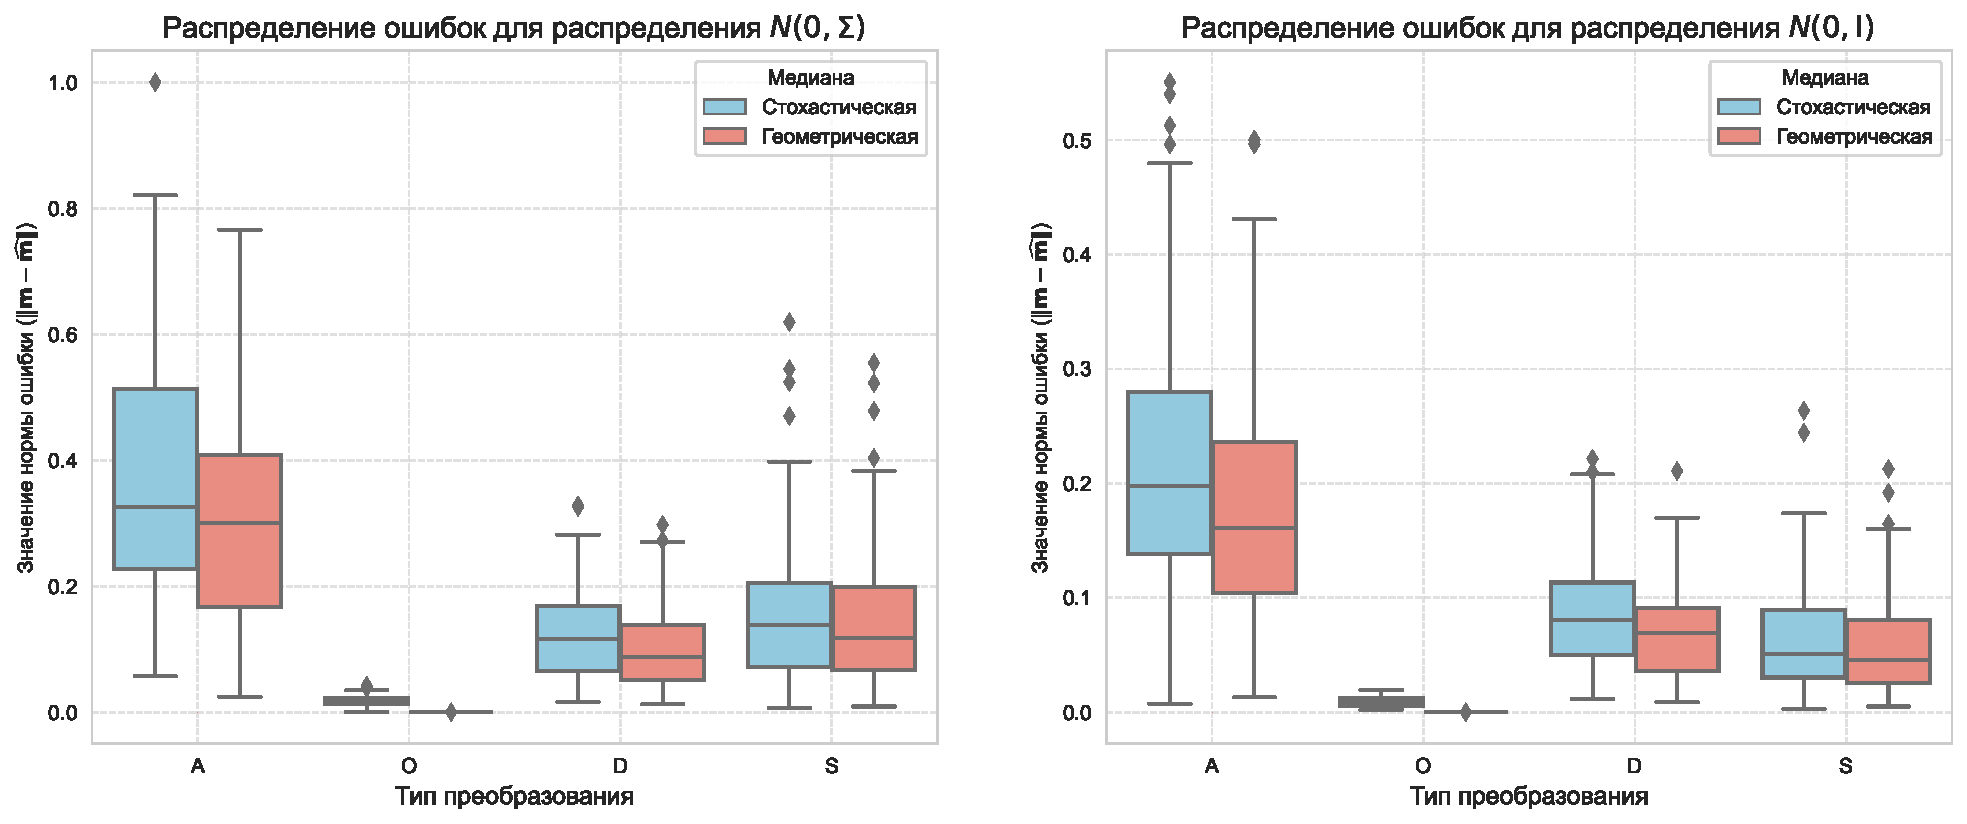
\includegraphics[width=15cm]{geom_exp_comp_equivariant.pdf}
  \caption{Сравнение распределений ошибок эквивариантности для алгоритма оценки геометрической медианы и предложенного алгоритма.}
  \label{fig:geom_exp_comp_equivariant}
\end{figure}

Результаты сравнения представлены на Рисунке~\ref{fig:geom_exp_comp_equivariant}. Видно, что для предложенного алгоритма ошибка близка к нулю только в случае ортогональных преобразований, причем данное свойство наблюдается для обоих рассматриваемых распределений. Это согласуется с результатами предыдущего раздела, где было показано, что алгоритм связан с проекционной медианой и методом yamm, обладающими эквивариантностью относительно поворотов.

Для диагональных преобразований и матриц сдвига ошибки остаются сравнительно малыми: медианные значения не превышают $0{,}1$. Однако в случае произвольных невырожденных преобразований ошибка возрастает примерно в два раза.

Для геометрической медианы наблюдается аналогичный характер поведения. При этом ошибки геометрической медианы в среднем несколько меньше, чем у предложенного алгоритма. Это указывает на необходимость дальнейшей доработки реализации стохастического алгоритма.

\section{Результаты работы алгоритма для различного вида областей и распределений}

% В предыдущих разделах были исследованы теоретические свойства предложенного алгоритма, а также его связь с проекционной медианой. Однако не менее важно понять, как алгоритм ведет себя на выборках различной природы.

% В данном разделе исследуется поведение предложенного алгоритма на выборках из непрерывных и дискретных распределений, а также в областях различной геометрии: выпуклых, невыпуклых и несвязных. 

В предыдущих разделах были исследованы теоретические свойства предложенного алгоритма и его связь с проекционной медианой. Далее рассмотрим поведение алгоритма на выборках различной природы: для непрерывных и дискретных распределений, а также в областях различной формы.

\subsection{Несвязная область}

Рассмотрим работу различных алгоритмов оценки параметра положения на выборке из равномерного распределения в несвязной области (Рисунок~\ref{fig:disjoint_1000}). Видно, что все алгоритмы, кроме медианы Оджа, дают близкие оценки, расположенные вблизи выборочного среднего. 

%Таким образом, наличие двух разделенных кластеров не оказывает существенного влияния на поведение большинства рассматриваемых методов.
\vspace{-0.5ex}

\begin{figure}[!hhh]
   \centering
    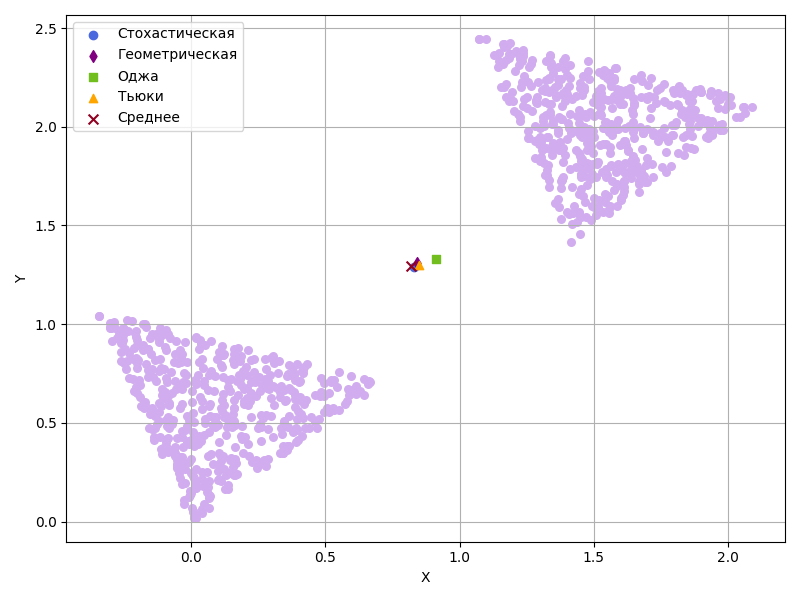
\includegraphics[width=0.95\textwidth]{sample_1000_med_and_mean.png}
  \caption{Сравнение различных оценок многомерной медианы для выборки объема 1000 из равномерного распределения в несвязной области.}
  \label{fig:disjoint_1000}
\end{figure}

\newpage

\subsection{Произвольная выпуклая область}

Далее рассмотрим выборку из равномерного распределения внутри выпуклой области (Рисунок~\ref{fig:convex}).

Как видно из рисунка, все рассматриваемые алгоритмы дают близкие оценки параметра положения, расположенные вблизи выборочного среднего. В данном случае различия между методами оказываются минимальными.


\begin{figure}[!hhh]
   \centering
    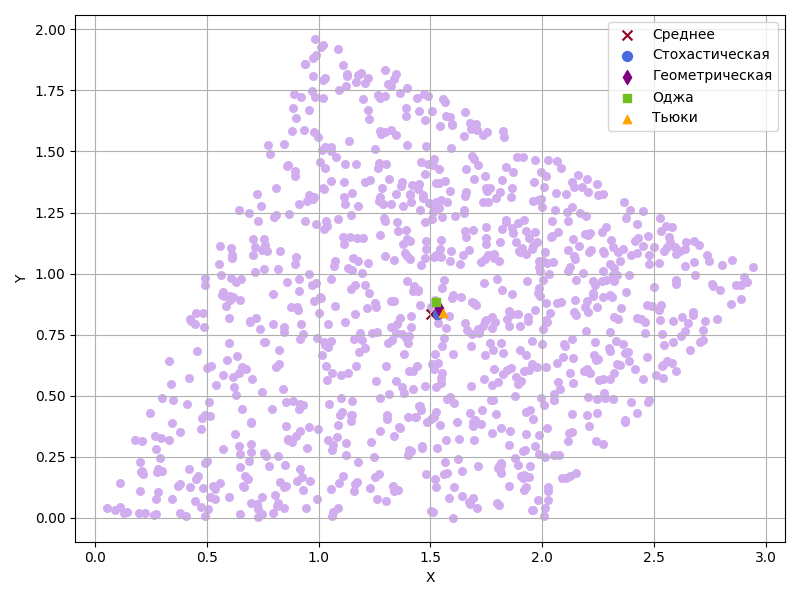
\includegraphics[width=0.95\textwidth]{sample_nonconvex.png}
  \caption{Сравнение различных оценок многомерной медианы для выборки объема 1000 из равномерного распределения в выпуклой области.} 
  \label{fig:convex}
\end{figure}
%\newpage

\subsection{Невыпуклые области}

\subsubsection{Невыпуклый пятиугольник}

Рассмотрим теперь случай равномерного распределения в невыпуклой области (Рисунок~\ref{fig:nonconvex_flag}).

Несмотря на невыпуклость области, все алгоритмы продолжают давать устойчивые оценки параметра положения, хотя наблюдается небольшое смещение относительно выборочного среднего. Это позволяет предположить, что отсутствие выпуклости у области само по себе не оказывает существенного влияния на работу рассматриваемых методов.


\begin{figure}[!hhh]
   \centering
    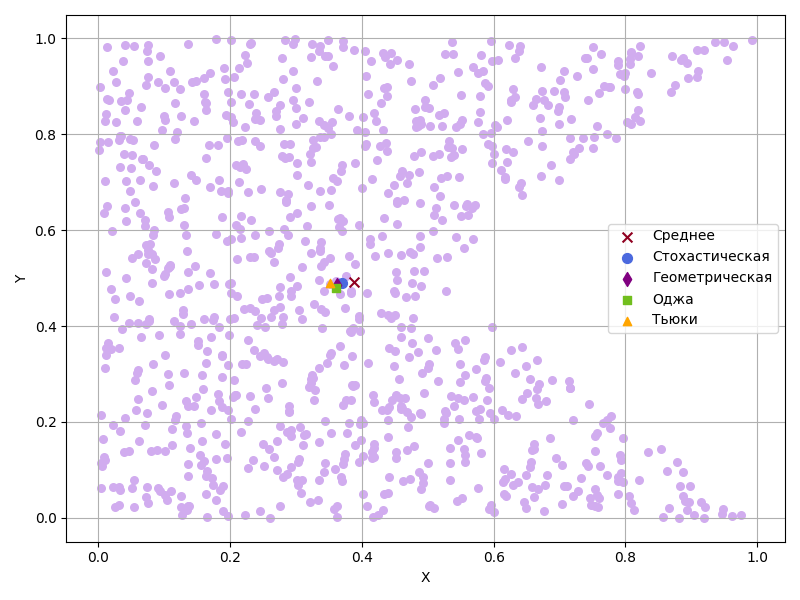
\includegraphics[width=0.95\textwidth]{sample_polygon.png}
  \caption{Сравнение различных оценок многомерной медианы для выборки объема 1000 из равномерного распределения в области в виде невыпуклого пятиугольника.
   % Сравнение различных оценок многомерной медианы для выборки объема 1000 в форме невыпуклого пятиугольника с равномерным распределением внутри области.
  }
  \label{fig:nonconvex_flag}
\end{figure}
%\newpage

\subsubsection{Кольцо}

Более интересная ситуация наблюдается в случае равномерного распределения в кольце (Рисунок~\ref{fig:ring}). Для данной выборки выборочное среднее, геометрическая медиана и медиана Тьюки дают практически совпадающие оценки, расположенные в центре области.

Предложенный алгоритм и медиана Оджа дают близкие между собой результаты, однако их оценки оказываются слегка смещенными относительно центра тяжести. Тем не менее, величина смещения остается незначительной.

\begin{figure}[!hhh]
   \centering
    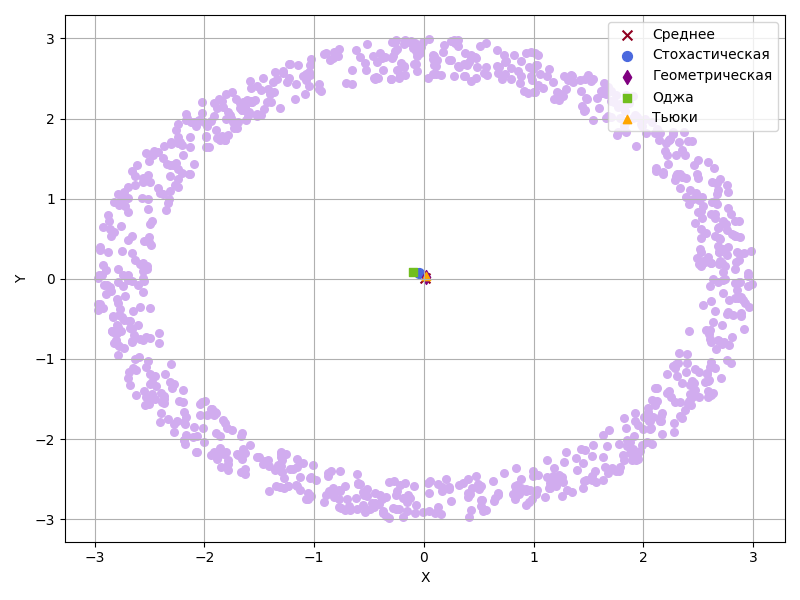
\includegraphics[width=0.95\textwidth]{sample_ring.png}
  \caption{Сравнение различных оценок многомерной медианы для выборки объема 1000 в форме кольца с равномерным распределением внутри области.}
  \label{fig:ring}
\end{figure}
\newpage

\subsection{Дискретные распределения}

Рассмотрим теперь дискретные распределения.

\vspace{-2ex}

\subsubsection{Пуассоновское двумерное}

Выборка из двумерного распределения Пуассона $X_{1},X_{2}$ получается следующим образом:  $X_{1}=Y_{1}+Y_{3},\ X_{2}=Y_{2}+Y_{3}$, где $Y_{1},Y_{2},Y_{3}$ --- независимые распределения Пуассона с параметрами $\lambda_{1},\lambda_{2},\lambda_{3}$.

Рассмотрим распределения Пуассона с параметрами $\lambda_{1} = 1,\ \lambda_{2}=2,\ $ $\lambda_{3}=3.$ Тогда параметры двумерного $\Lambda_{1}=4,\ \Lambda_{2}=5$, из чего следует, что  математическое ожидание распределения равно $(4; 5)^{\mathrm{T}}$.

Из Рисунка~\ref{fig:poisson} видно, что медианы Тьюки и Оджа, а также выборочное среднее дают практически совпадающие оценки, близкие к теоретическому математическому ожиданию. Предложенный алгоритм и геометрическая медиана также дают близкие результаты, хотя наблюдается небольшое смещение.

\begin{figure}[!hhh]
   \centering
    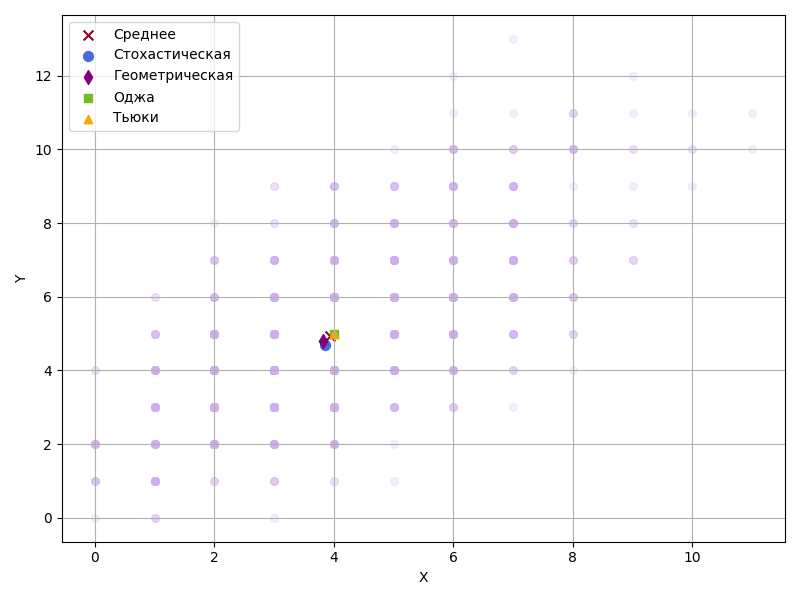
\includegraphics[width=0.9 \textwidth]{sample_poisson.png}
  \caption{Сравнение различных оценок многомерной медианы для дискретной выборки объема 1000 из двумерного распределения Пуассона с параметрами $\Lambda_{1}=4,\ \Lambda_{2}=5$. }
  \label{fig:poisson}
\end{figure}
\newpage

\subsubsection{Дискретное двумерное}

Рассмотрим теперь двумерное распределение следующего вида. Выборка генерируется как геометрическое распределение с параметром $p_1 = 0{,}5$ по первой оси и с параметром $p_2 = 0{,}2$ по второй. В этом случае математическое ожидание равно $(2; 5)^{\mathrm{T}}$.

Как видно из Рисунка~\ref{fig:geom}, только выборочное среднее совпадает с теоретическим математическим ожиданием. Остальные алгоритмы дают близкие между собой оценки, смещенные в одну сторону. Наибольшее смещение наблюдается у медианы Тьюки.

Вероятно, данное поведение связано с асимметрией распределения и дискретной природой выборки.
\newpage
\begin{figure}[!hhh]
   \centering
    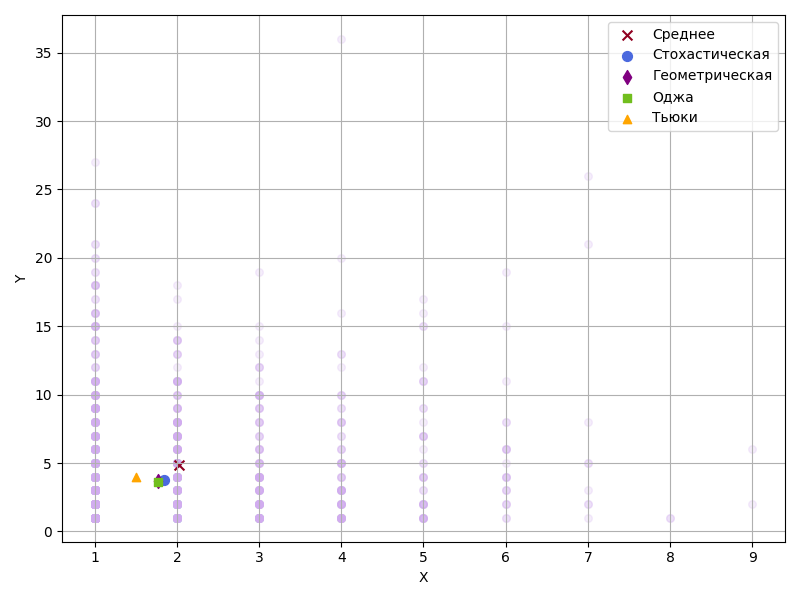
\includegraphics[width=0.95\textwidth]{sample_geom.png}
  \caption{Сравнение различных оценок многомерной медианы для дискретной выборки объема 1000, где распределение по каждой оси геометрическое с параметрами $p_1 = 0{,}5$ по первой оси и $p_2 = 0{,}2$ по второй.}
  \label{fig:geom}
\end{figure}

\vspace{2ex}

Таким образом, проведенные эксперименты показывают, что предложенный алгоритм демонстрирует устойчивое поведение для широкого класса распределений и областей. В большинстве рассмотренных примеров предложенный алгоритм дает оценки, сопоставимые с геометрической медианой, что согласуется с результатами предыдущих исследований.
\chapter{Модификации алгоритма оценки параметра положения}

Практическое применение представленного в главе~2 Алгоритма~\ref{alg:median}  осложняется рядом проблем, связанных с его стохастической природой. Во-первых, качество работы алгоритма существенно зависит от выбора критерия останова. Во-вторых, случайность направлений приводит к относительно большому разбросу финальной оценки и может вызывать преждевременную остановку алгоритма. Кроме того, вблизи истинного параметра положения последовательные приближения начинают колебаться между несколькими точками, что препятствует достижению высокой точности.

Для устранения этих проблем в данной главе рассматриваются модификации алгоритма, направленные на повышение устойчивости и точности оценки, а также на улучшение практической применимости метода.

\section{Повышение устойчивости оценки}

\subsection{Изменение критерия останова}

В Алгоритме~\ref{alg:median} используется абсолютный критерий останова, который сравнивает норму разницы последовательных приближений с заданной точностью~$\varepsilon$: 
\[ \|\widehat{\mathbf{m}}_{{i}}-\widehat{\mathbf{m}}_{{i+1}}\|<\varepsilon.\]

Однако такой критерий имеет существенный недостаток --- он не учитывает масштаб данных. Это может привести к следующим проблемам:

\begin{itemize}
    \item Для данных с большим масштабом алгоритм может выполнять слишком много итераций после достижения практически значимой точности.
    \item Для данных малого масштаба алгоритм может остановиться слишком рано, не достигнув достаточной точности.
\end{itemize}

Для устранения этой проблемы предлагается использовать относительный критерий останова, который не чувствителен к масштабу данных:
\[ \|\widehat{\mathbf{m}}_{{i}}-\widehat{\mathbf{m}}_{{i+1}}\|<\varepsilon \cdot \|\widehat{\mathbf{m}}_{{i}}\|.\]

Рассмотрим работу алгоритма с абсолютным и относительным критериями останова на выборке объема 1000 из многомерного нормального распределения с нулевым математическим ожиданием и ковариационной матрицей~\eqref{eq:experimentmatrix}\footnote{Далее в разделе все сравнения проводятся именно для данного распределения, если не оговорено обратное.}.

Выбранное распределение соответствует одному из наиболее неблагоприятных случаев для алгоритма: данные обладают различными дисперсиями и при этом являются коррелированными. Это позволит наглядно продемонстрировать масштабную инвариантность относительного критерия в сравнении с абсолютным. Кроме того, размерность $d=3$ является более показательной по сравнению с двумерным случаем.

В Таблице~\ref{table: abs_rel_crit_eps} приведены минимальные, максимальные значения и значения квартилей нормы разности между полученной алгоритмом оценкой и истинным значением медианы для различных комбинаций критерия останова, точности $\varepsilon$ и масштаба данных. Здесь Sample обозначает исходную выборку из распределения, описанного выше, Sample$/100$ --- ту же выборку, делённую на 100, а Sample$\,\cdot 100$ --- умноженную на 100. Моделирование выборки Sample проводилось 100 раз. 

Однако при сравнении критериев останова важно учитывать не только точность оценки, но и количество итераций, необходимое для выполнения условия останова. Соответствующие результаты приведены в Таблице~\ref{table: abs_rel_crit_iter}, где представлены минимальные, максимальные значения и значения квартилей числа итераций для различных значений $\varepsilon$ и масштабов данных.

На основании представленных в Таблицах~\ref{table: abs_rel_crit_eps} и~\ref{table: abs_rel_crit_iter} результатов можно сделать следующие выводы.

\begin{table}[!hhh]
 \caption{Сравнение точности для разных критериев останова}
    \label{table: abs_rel_crit_eps}
\centering
\begin{tabular}{|c|c|c|c|c|c|}
\hline
\multicolumn{2}{|c|}{\textbf{Критерий}} & \multicolumn{2}{c|}{\textbf{абсолютный}} & \multicolumn{2}{c|}{\textbf{относительный}} \\
\hline
\textbf{Выборка} & \textbf{Точность} & $10^{-2}$ & $10^{-3}$ & $10^{-2}$ & $10^{-3}$ \\
\hline
\multirow{5}{*}{Sample$/100$} & min & $8,235 \cdot 10^{-4}$ & $4,071 \cdot 10^{-4}$ & $4,576 \cdot 10^{-4}$ & $1,168 \cdot 10^{-4}$ \\
\cline{2-6}
& 0,25 & $1,095 \cdot 10^{-2}$ & $2,396 \cdot 10^{-3}$ & $1,003 \cdot 10^{-3}$ & $1,035 \cdot 10^{-3}$ \\
\cline{2-6}
& 0,5 & $1,669 \cdot 10^{-2}$ & $4,722 \cdot 10^{-3}$ & $1,478 \cdot 10^{-3}$ & $1,385 \cdot 10^{-3}$ \\
\cline{2-6}
& 0,75 & $2,781 \cdot 10^{-2}$ & $1,191 \cdot 10^{-2}$ & $2,160 \cdot 10^{-3}$ & $1,880 \cdot 10^{-3}$ \\
\cline{2-6}
& max & $7,279 \cdot 10^{-2}$ & $5,277 \cdot 10^{-2}$ & $9,579 \cdot 10^{-3}$ & $3,217\cdot 10^{-3}$ \\
\hline

\multirow{5}{*}{Sample} & min & $4,071 \cdot 10^{-2}$ & $4,576 \cdot 10^{-2}$ & $4,576 \cdot 10^{-2}$ & $1,168 \cdot 10^{-2}$ \\
\cline{2-6}
& 0,25 & $1,035 \cdot 10^{-1}$ & $9,097 \cdot 10^{-2}$ & $1,003 \cdot 10^{-1}$ & $1,035 \cdot 10^{-1}$ \\
\cline{2-6}
& 0,5 & $1,433 \cdot 10^{-1}$ & $1,289 \cdot 10^{-1}$ & $1,478 \cdot 10^{-1}$ & $1,385 \cdot 10^{-1}$ \\
\cline{2-6}
& 0,75 & $2,379 \cdot 10^{-1}$ & $1,717 \cdot 10^{-1}$ & $2,160 \cdot 10^{-1}$ & $1,880 \cdot 10^{-1}$ \\
\cline{2-6}
& max & $1,531 $ & $4,832 \cdot 10^{-1}$ & $9,579  \cdot 10^{-1} $ & $3,217  \cdot 10^{-1} $ \\
\hline

\multirow{5}{*}{Sample$\, \cdot 100$} & min & $1,168$ & $1,168$ & $4,576$ & $1,168$ \\
\cline{2-6}
& 0,25 & $8,454$ & $7,579$ & $10,03$ & $10,35$ \\
\cline{2-6}
& 0,5 & $12,34$ & $12,02$ & $14,78$ & $13,85$ \\
\cline{2-6}
& 0,75 & $16,42$ & $16,29$ & $21,60$ & $18,80$ \\
\cline{2-6}
& max & $29,14$ & $29,14$ & $95,79$ & $32,17$ \\
\hline
\end{tabular}
\end{table}


% \begin{table}[!hhh]
%  \caption{Сравнение точности для разных критериев останова}
%     \label{table: abs_rel_crit_eps}
% \centering
% \begin{tabular}{|c|c|c|c|c|c|}
% \hline
% \multicolumn{2}{|c|}{\textbf{Критерий}} & \multicolumn{2}{c|}{\textbf{абсолютный}} & \multicolumn{2}{c|}{\textbf{относительный}} \\
% \hline
% \textbf{Выборка} & \textbf{Точность} & $10^{-2}$ & $10^{-3}$ & $10^{-2}$ & $10^{-3}$ \\
% \hline
% \multirow{5}{*}{Sample$/100$} & min & $4,12 \cdot 10^{-4}$ & $4,12  \cdot  10^{-4}$ & $3,47 \cdot  10^{-4}$ & $3,47 \cdot 10^{-4}$ \\
% \cline{2-6}
% & 0,25 & $1,375 \cdot 10^{-3}$   &  $1,296 \cdot 10^{-3}$ & $1,015\cdot 10^{-3}$  &  $0,947 \cdot 10^{-3}$ \\
% \cline{2-6}
% & 0,5 &  $2,234\cdot 10^{-3}$  &   $1,745\cdot 10^{-3}$ &  $1,361\cdot 10^{-3}$ &  $1,354\cdot 10^{-3}$   \\
% \cline{2-6}
% & 0,75 & $4,137\cdot 10^{-3}$ &  $2,797\cdot 10^{-3}$ & $1,756\cdot 10^{-3}$ &  $1,817\cdot 10^{-3}$ \\
% \cline{2-6}
% & max & $14,715\cdot 10^{-3}$ & $9,64\cdot 10^{-3}$ & $9,579\cdot 10^{-3}$ & $3,217\cdot 10^{-3}$ \\
% \hline

% \multirow{5}{*}{Sample} & min & $2,889 \cdot 10^{-2}$ & $3,105  \cdot  10^{-2}$ & $3,47 \cdot  10^{-2}$ & $3,47 \cdot 10^{-2}$ \\
% \cline{2-6}
% & 0,25 & $0,999 \cdot 10^{-1}$   &  $0,947 \cdot 10^{-1}$ & $1,015\cdot 10^{-1}$  &  $0,947 \cdot 10^{-1}$ \\
% \cline{2-6}
% & 0,5 &  $1,379\cdot 10^{-1}$  &   $1,224\cdot 10^{-1}$ &  $1,361\cdot 10^{-1}$ &  $1,354\cdot 10^{-1}$   \\
% \cline{2-6}
% & 0,75 & $1,731 \cdot 10^{-1}$ &  $1,625 \cdot 10^{-1}$ & $1,756\cdot 10^{-1}$ &  $1,817\cdot 10^{-1}$ \\
% \cline{2-6}
% & max & $9,579 \cdot 10^{-1}$ & $3,217 \cdot 10^{-1}$ & $9,579\cdot 10^{-1}$ & $3,217\cdot 10^{-1}$ \\
% \hline

% \multirow{5}{*}{Sample$\, \cdot 100$} & min & $1,81$ & $3,28$ & $3,47$ & $3,47$ \\
% \cline{2-6}
% & 0,25 & $9,17$ & $7,86$  & $10,15$  &  $9,47$ \\
% \cline{2-6}
% & 0,5 &  $11,98$  &   $11,83$ &  $13,61$ &  $13,54$   \\
% \cline{2-6}
% & 0,75 & $16,89$ &  $16,71$ & $17,56$ &  $18,17$ \\
% \cline{2-6}
% & max & $32,17$ & $34,04$ & $95,79$ & $32,17$ \\
% \hline
% \end{tabular}
% \end{table}

\newpage

\begin{itemize}
   \item \textbf{Сравнение критериев по точности}
      \begin{itemize}
         \item  Оба критерия показали сопоставимые результаты для разных масштабов. Однако для выборки Sample$/100$ относительный критерий показывает более стабильные результаты: разброс между квартилями оказывается меньше, а медианная ошибка --- ниже. 
         \item Ошибка относительного критерия меняется предсказуемо, а именно уменьшается (увеличивается) пропорционально данным, что отражает его масштабную инвариантность.
      \end{itemize}
      \end{itemize}

\newpage

% \begin{table}[h!]
%  \caption{Сравнение количества итераций до выполнения критерия останова}
%    \label{table: abs_rel_crit_iter}
% \centering
% \begin{tabular}{|c|c|c|c|c|c|}
% \hline
% \multicolumn{2}{|c|}{\textbf{Критерий}} & \multicolumn{2}{c|}{\textbf{абсолютный}} & \multicolumn{2}{c|}{\textbf{относительный}} \\
% \hline
% \textbf{Выборка} & \textbf{Точность} & $10^{-2}$ & $10^{-3}$ & $10^{-2}$ & $10^{-3}$ \\
% \hline
% \multirow{5}{*}{Sample$/100$} & min & $10$ & $10$ & $12$ & $17$ \\
% \cline{2-6}
% & 0,25 & $10$ & $10$ & $28,75$ & $173,75$ \\
% \cline{2-6}
% & 0,5 &  $10$ & $10,5$ & $47$ & $486$ \\
% \cline{2-6}
% & 0,75 & $10$ & $12$ & $81,75$ & $1019,25$ \\
% \cline{2-6}
% & max & $11$ & $17$ & $265$ & $2374$ \\
% \hline

% \multirow{5}{*}{Sample} & min & $10$ & $13$ & $12$ & $17$ \\
% \cline{2-6}
% & 0,25 & $13$ & $36,75$ & $28,75$ & $173,75$ \\
% \cline{2-6}
% & 0,5 &  $17,5$ & $55$ & $47$ & $486$ \\
% \cline{2-6}
% & 0,75 & $21$ & $93,25$ & $81,75$ & $1019,25$ \\
% \cline{2-6}
% & max & $38$ & $213$ & $265$ & $2374$ \\
% \hline

% \multirow{5}{*}{Sample$\, \cdot 100$} & min & $18$ & $18$ & $12$ & $17$ \\
% \cline{2-6}
% & 0,25 & $242,25$ & $2077$ & $28,75$ & $173,75$ \\
% \cline{2-6}
% & 0,5 &  $609$ & $4481,5$ & $47$ & $486$ \\
% \cline{2-6}
% & 0,75 & $1223,25$ & $10019,25$ & $81,75$ & $1019,25$ \\
% \cline{2-6}
% & max & $4413$ & $33131$ & $265$ & $2374$ \\
% \hline

% \end{tabular}
% \end{table}


\begin{table}[!hhh]
 \caption{Сравнение количества итераций до выполнения критерия останова}
   \label{table: abs_rel_crit_iter}
\centering
\begin{tabular}{|c|c|c|c|c|c|}
\hline
\multicolumn{2}{|c|}{\textbf{Критерий}} & \multicolumn{2}{c|}{\textbf{абсолютный}} & \multicolumn{2}{c|}{\textbf{относительный}} \\
\hline
\textbf{Выборка} & \textbf{Точность} & $10^{-2}$ & $10^{-3}$ & $10^{-2}$ & $10^{-3}$ \\
\hline
\multirow{5}{*}{Sample$/100$} & min & $1$ & $1$ & $1$ & $5$ \\
\cline{2-6}
& 0,25 & $1$ & $4$ & $16$ & $153,8$ \\
\cline{2-6}
& 0,5 & $2$ & $6$ & $42,5$ & $470$ \\
\cline{2-6}
& 0,75 & $3$ & $8,2$ & $71,8$ & $688,5$ \\
\cline{2-6}
& max & $5$ & $16$ & $240$ & $2276$ \\
\hline

\multirow{5}{*}{Sample} & min & $4$ & $5$ & $1$ & $5$ \\
\cline{2-6}
& 0,25 & $9,8$ & $30$ & $16$ & $153,8$ \\
\cline{2-6}
& 0,5 & $15$ & $51,5$ & $42,5$ & $470$ \\
\cline{2-6}
& 0,75 & $20$ & $93,2$ & $71,8$ & $688,5$ \\
\cline{2-6}
& max & $43$ & $317$ & $240$ & $2276$ \\
\hline

\multirow{5}{*}{Sample$\, \cdot 100$} & min & $22$ & $81$ & $1$ & $5$ \\
\cline{2-6}
& 0,25 & $200$ & $1969$ & $16$ & $153,8$ \\
\cline{2-6}
& 0,5 & $532,5$ & $4175$ & $42,5$ & $470$ \\
\cline{2-6}
& 0,75 & $788,8$ & $8084,8$ & $71,8$ & $688,5$ \\
\cline{2-6}
& max & $4848$ & $33382$ & $240$ & $2276$ \\
\hline
\end{tabular}
\end{table}


\begin{itemize}
   \item \textbf{Сравнение критериев по количеству итераций}
      \begin{itemize}
         \item Для относительного критерия распределение числа итераций практически не зависит от масштаба данных. В случае абсолютного критерия наблюдается противоположное поведение. Для выборки Sample$/100$ алгоритм с абсолютным критерием завершается за очень малое количество шагов. Это связано с тем, что фиксированное значение $\varepsilon$ становится слишком маленьким относительно масштаба данных, что приводит к преждевременной остановке алгоритма.
      
         \item Напротив, для выборки Sample$\,\cdot 100$ количество итераций для абсолютного критерия резко возрастает и существенно превышает число итераций относительного критерия при сопоставимой точности.
      \end{itemize}
\end{itemize}

Таким образом, относительный критерий останова является значительно более устойчивым к изменению масштаба данных, что делает его предпочтительным для практического применения.

Тем не менее, как видно из Таблицы~\ref{table: abs_rel_crit_eps}, относительный критерий при больших значениях $\varepsilon$ может давать результаты, значительно отличающиеся от ожидаемых (значения $95{,}79$ и $9{,}579\cdot 10^{-1}$). Следовательно, для существенного повышения устойчивости алгоритма одной замены критерия останова недостаточно.

\subsection{Условие на минимальное количество итераций}

Несмотря на то, что относительный критерий останова позволяет устранить зависимость от масштаба данных, проблема преждевременной остановки алгоритма полностью не исчезает. Из-за случайности направлений критерий останова может выполниться случайно уже на ранних итерациях, когда алгоритм еще находится далеко от оптимума. Это приводит к появлению выбросов ошибки и увеличению разброса итоговой оценки.

Для уменьшения вероятности преждевременной остановки рассмотрим следующую модификацию: алгоритм обязан выполнить заданное минимальное количество итераций, даже если критерий останова выполняется раньше.

Пусть $k_{min}$ --- минимальное количество итераций, которое алгоритм должен выполнить. Тогда Алгоритм~\ref{alg:median} продолжает работу до тех пор, пока одновременно не выполнены условия $i \geqslant k_{min}$ и $\|\widehat{\mathbf{m}}_{{i}}-\widehat{\mathbf{m}}_{{i+1}}\|<\varepsilon \cdot \|\widehat{\mathbf{m}}_{{i}}\|$. Таким образом, до достижения $k_{min}$ критерий останова фактически игнорируется. После выполнения условия $i \geqslant k_{min}$ алгоритм продолжает работу так же, как и в исходной версии.

Данная модификация не изменяет сам принцип работы алгоритма, однако позволяет уменьшить вероятность случайной ранней остановки, вызванной удачным выбором направлений на первых итерациях.

На Рисунке~\ref{fig:k_min} представлены распределения нормы ошибки $\|\mathbf{m}-\widehat{\mathbf{m}}\|$ для различных значений $k_{min}\in\{0,5,10,20\}$, где $k_{min}=0$ соответствует исходному алгоритму с относительным критерием останова.

\begin{figure}[!hhh]
   \centering
    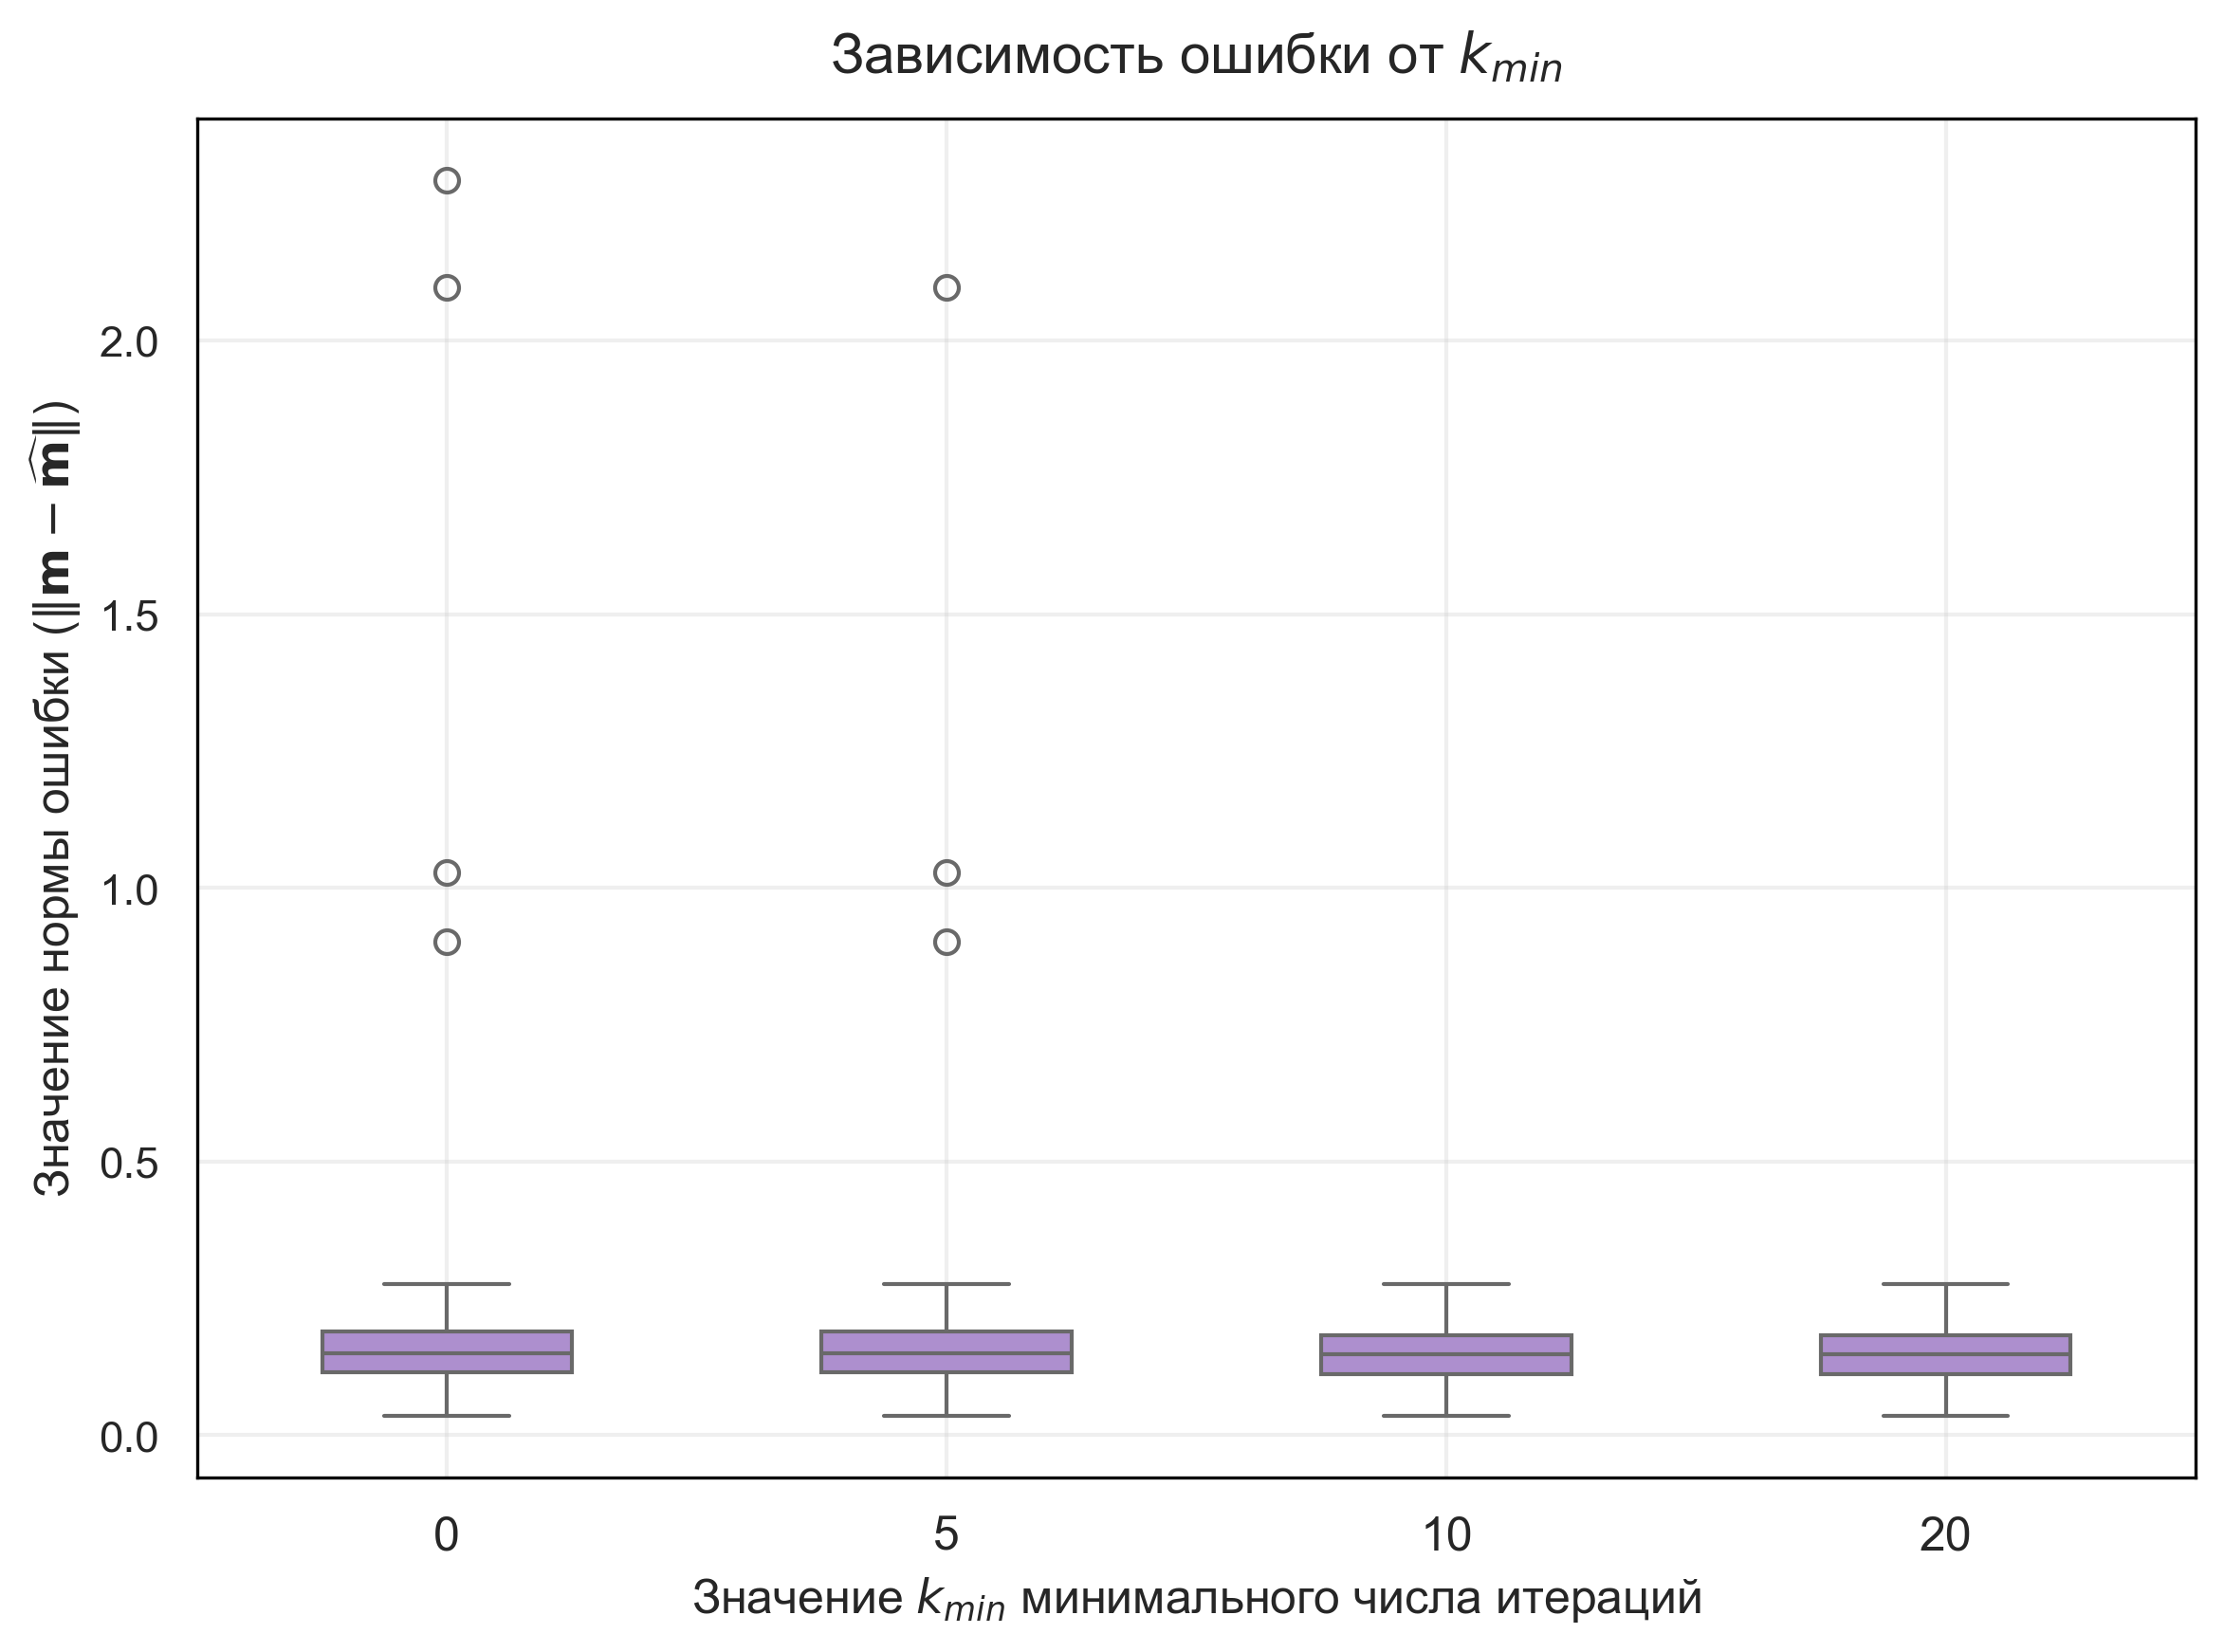
\includegraphics[width=0.8\textwidth]{stochastic_median_k_min_boxplots.png}
  \caption{Распределения ошибок модификации алгоритма для различных значений минимального числа итераций $k_{min}\in\{0,5,10,20\}$.}
  \label{fig:k_min}
\end{figure}

Видно, что увеличение минимального числа итераций практически не влияет на медианное значение ошибки и межквартильный размах распределения. Однако при $k_{min}=0$ и $k_{min}=5$ наблюдаются выбросы, соответствующие случаям преждевременной остановки алгоритма. При $k_{min}\geqslant 10$ подобные выбросы исчезают. 

Таким образом, введение минимального числа итераций позволяет существенно уменьшить вероятность крупных ошибок, связанных с преждевременной остановкой алгоритма, при этом практически не изменяя основные характеристики распределения ошибок.

\subsection{Многократное выполнение критерия останова}

В предыдущем разделе было показано, что введение минимального числа итераций позволяет уменьшить количество крупных ошибок, возникающих из-за преждевременной остановки алгоритма. Однако случайное выполнение критерия останова все еще возможно до достижения реальной сходимости.

Для дальнейшего повышения устойчивости рассмотрим следующую модификацию: алгоритм завершается только после того, как критерий останова выполнится  $c$ раз.

Пусть $c$ --- число выполнений критерия останова, необходимых для завершения алгоритма. На каждой итерации проверяется условие $\|\widehat{\mathbf{m}}_{{i}}-\widehat{\mathbf{m}}_{{i+1}}\|<\varepsilon \cdot \|\widehat{\mathbf{m}}_{{i}}\|$, если оно выполнено, то счетчик успешных проверок увеличивается на единицу. Алгоритм завершается только тогда, когда число выполнений критерия достигает значения $c$.

При $c=1$ получаем исходный вариант алгоритма с относительным критерием останова. Таким образом, данная модификация является естественным обобщением предыдущего подхода.

Рассмотрим работу алгоритма для значений $c\in\{1, 2, 3, 4, 5\}$.

\begin{figure}[!h]
   \centering
    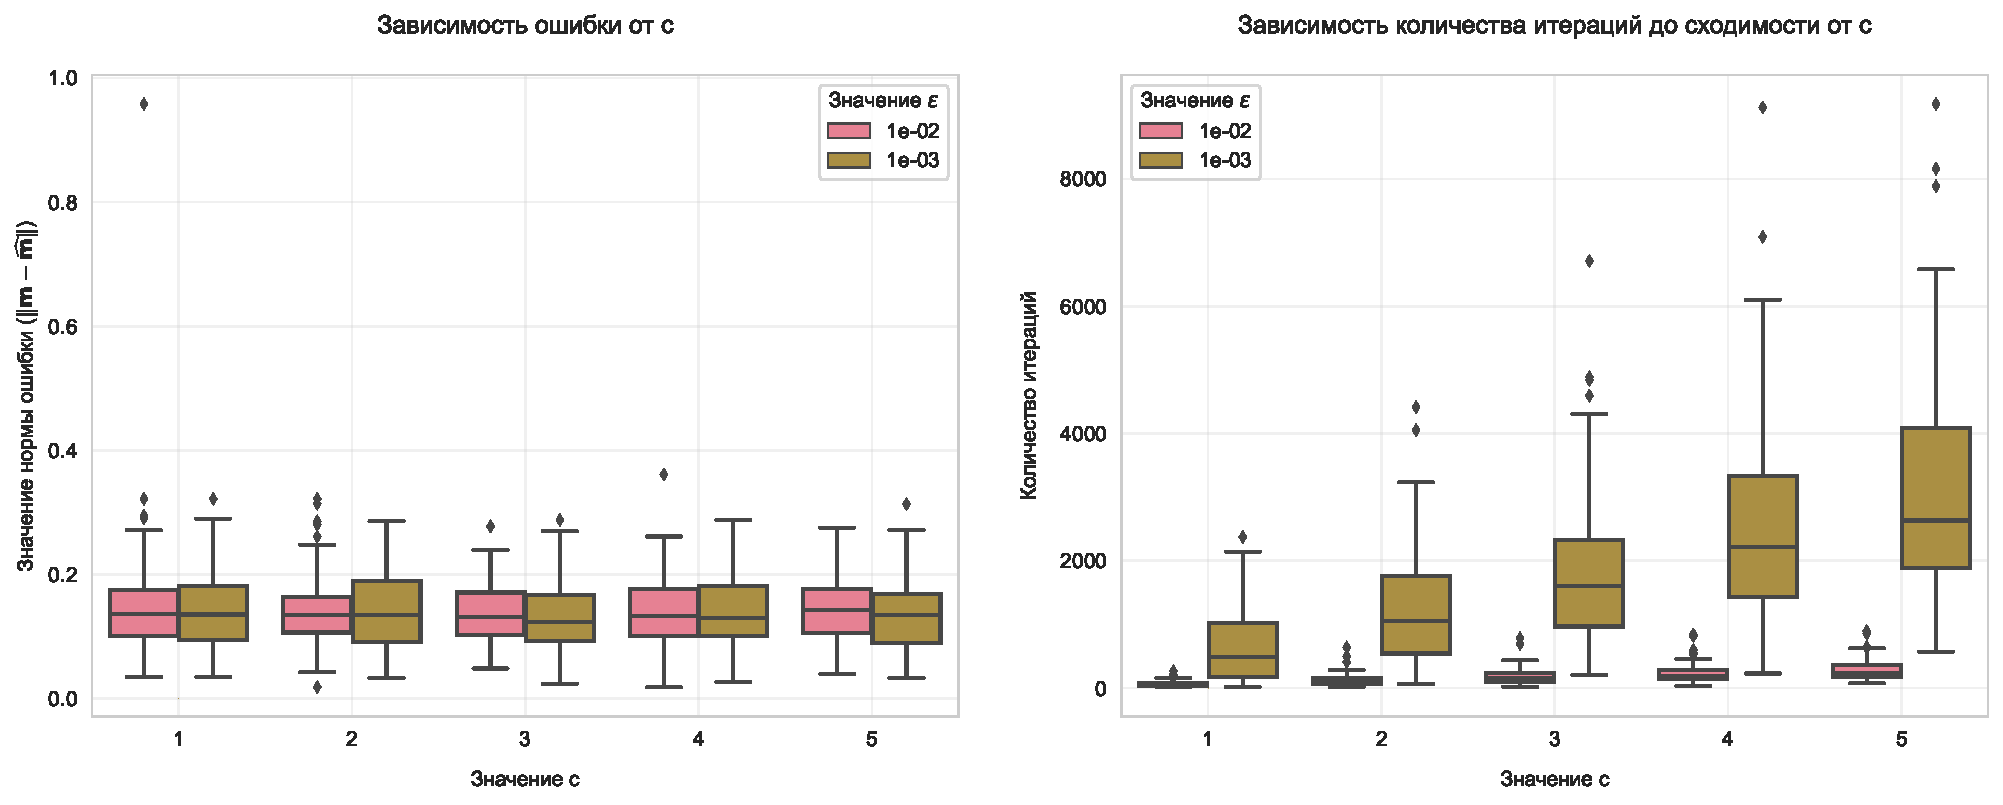
\includegraphics[width=15cm]{comp_stable_crit_results_out_5.pdf}
  \caption{Распределения ошибок и числа итераций для различных значений параметра $c$, где $c\in\{1, 2, 3, 4, 5\}$ --- число выполнений критерия останова, необходимых для завершения алгоритма.}
  \label{fig:comp_stable_crit_results_out_5}
\end{figure}

Результаты, представленные на рисунке~\ref{fig:comp_stable_crit_results_out_5}, показывают, что увеличение параметра $c$ позволяет практически устранить случаи преждевременной остановки алгоритма, приводящие к значительным ошибкам.  Однако точность при таком подходе повышается совсем незначительно. 

Также видно, что с ростом $c$ существенно увеличивается число итераций, необходимое для завершения алгоритма. Однако уменьшения разброса ошибок при больших значениях $c$ практически не наблюдается. Поэтому в данном случае использование значений $c>3$ оказывается практически неоправданным.

\section{Повышение точности оценки}

Предыдущие модификации были направлены прежде всего на повышение устойчивости алгоритма и уменьшение вероятности преждевременной остановки. Однако даже после достижения критерия останова финальная оценка все еще существенно зависит от случайного выбора направлений. Кроме того, вблизи оптимума последовательные приближения алгоритма начинают колебаться около истинного параметра положения. Поэтому использование только последней итерации может приводить к дополнительному разбросу оценки.

В данном разделе рассматриваются модификации, направленные непосредственно на повышение точности финальной оценки.

\subsection{Усреднение последних итераций}

Данная модификация основана на усреднении нескольких последних приближений алгоритма. Вместо использования результата последней итерации Алгоритма~\ref{alg:median} предлагается после достижения заданной точности $\varepsilon$ выполнить еще ${\text{w}}$ итераций и усреднить полученные оценки.

Пусть $N$ --- число итераций, необходимое для достижения критерия останова в Алгоритме~\ref{alg:median}, а ${\text{w}}$ --- число усредняемых итераций. Получаем последовательность приближений $\{\widehat{\mathbf{m}}_{{i}}\}_{i=N+1}^{N+{\text{w}}}$. Финальная оценка вычисляется по формуле
\[\widehat{\mathbf{m}}_{\text{avg}_{\text{w}}} = \frac{1}{{\text{w}}} \sum_{i=N+1}^{N+{\text{w}}} \widehat{\mathbf{m}}_{{i}}. \]


Усреднение последних итераций позволяет уменьшить влияние случайных колебаний отдельных итераций, тем самым снижая разброс финальной оценки.

Для исследования влияния параметра ${\text{w}}$ рассмотрим значения \\
${\text{w}}\in\{0,5,10,20\}$, где ${\text{w}}=0$ соответствует исходному алгоритму без усреднения.

На Рисунке~\ref{fig:additional_steps_boxplots} представлены распределения нормы ошибки для различных значений параметра ${\text{w}}$.

Видно, что увеличение числа усредняемых итераций приводит к уменьшению медианного значения ошибки, а также к небольшому уменьшению межквартильного размаха распределения. При этом наиболее заметное улучшение наблюдается при переходе от ${\text{w}}=0$ к ${\text{w}}=5$.

\begin{figure}[!hhh]
   \centering
    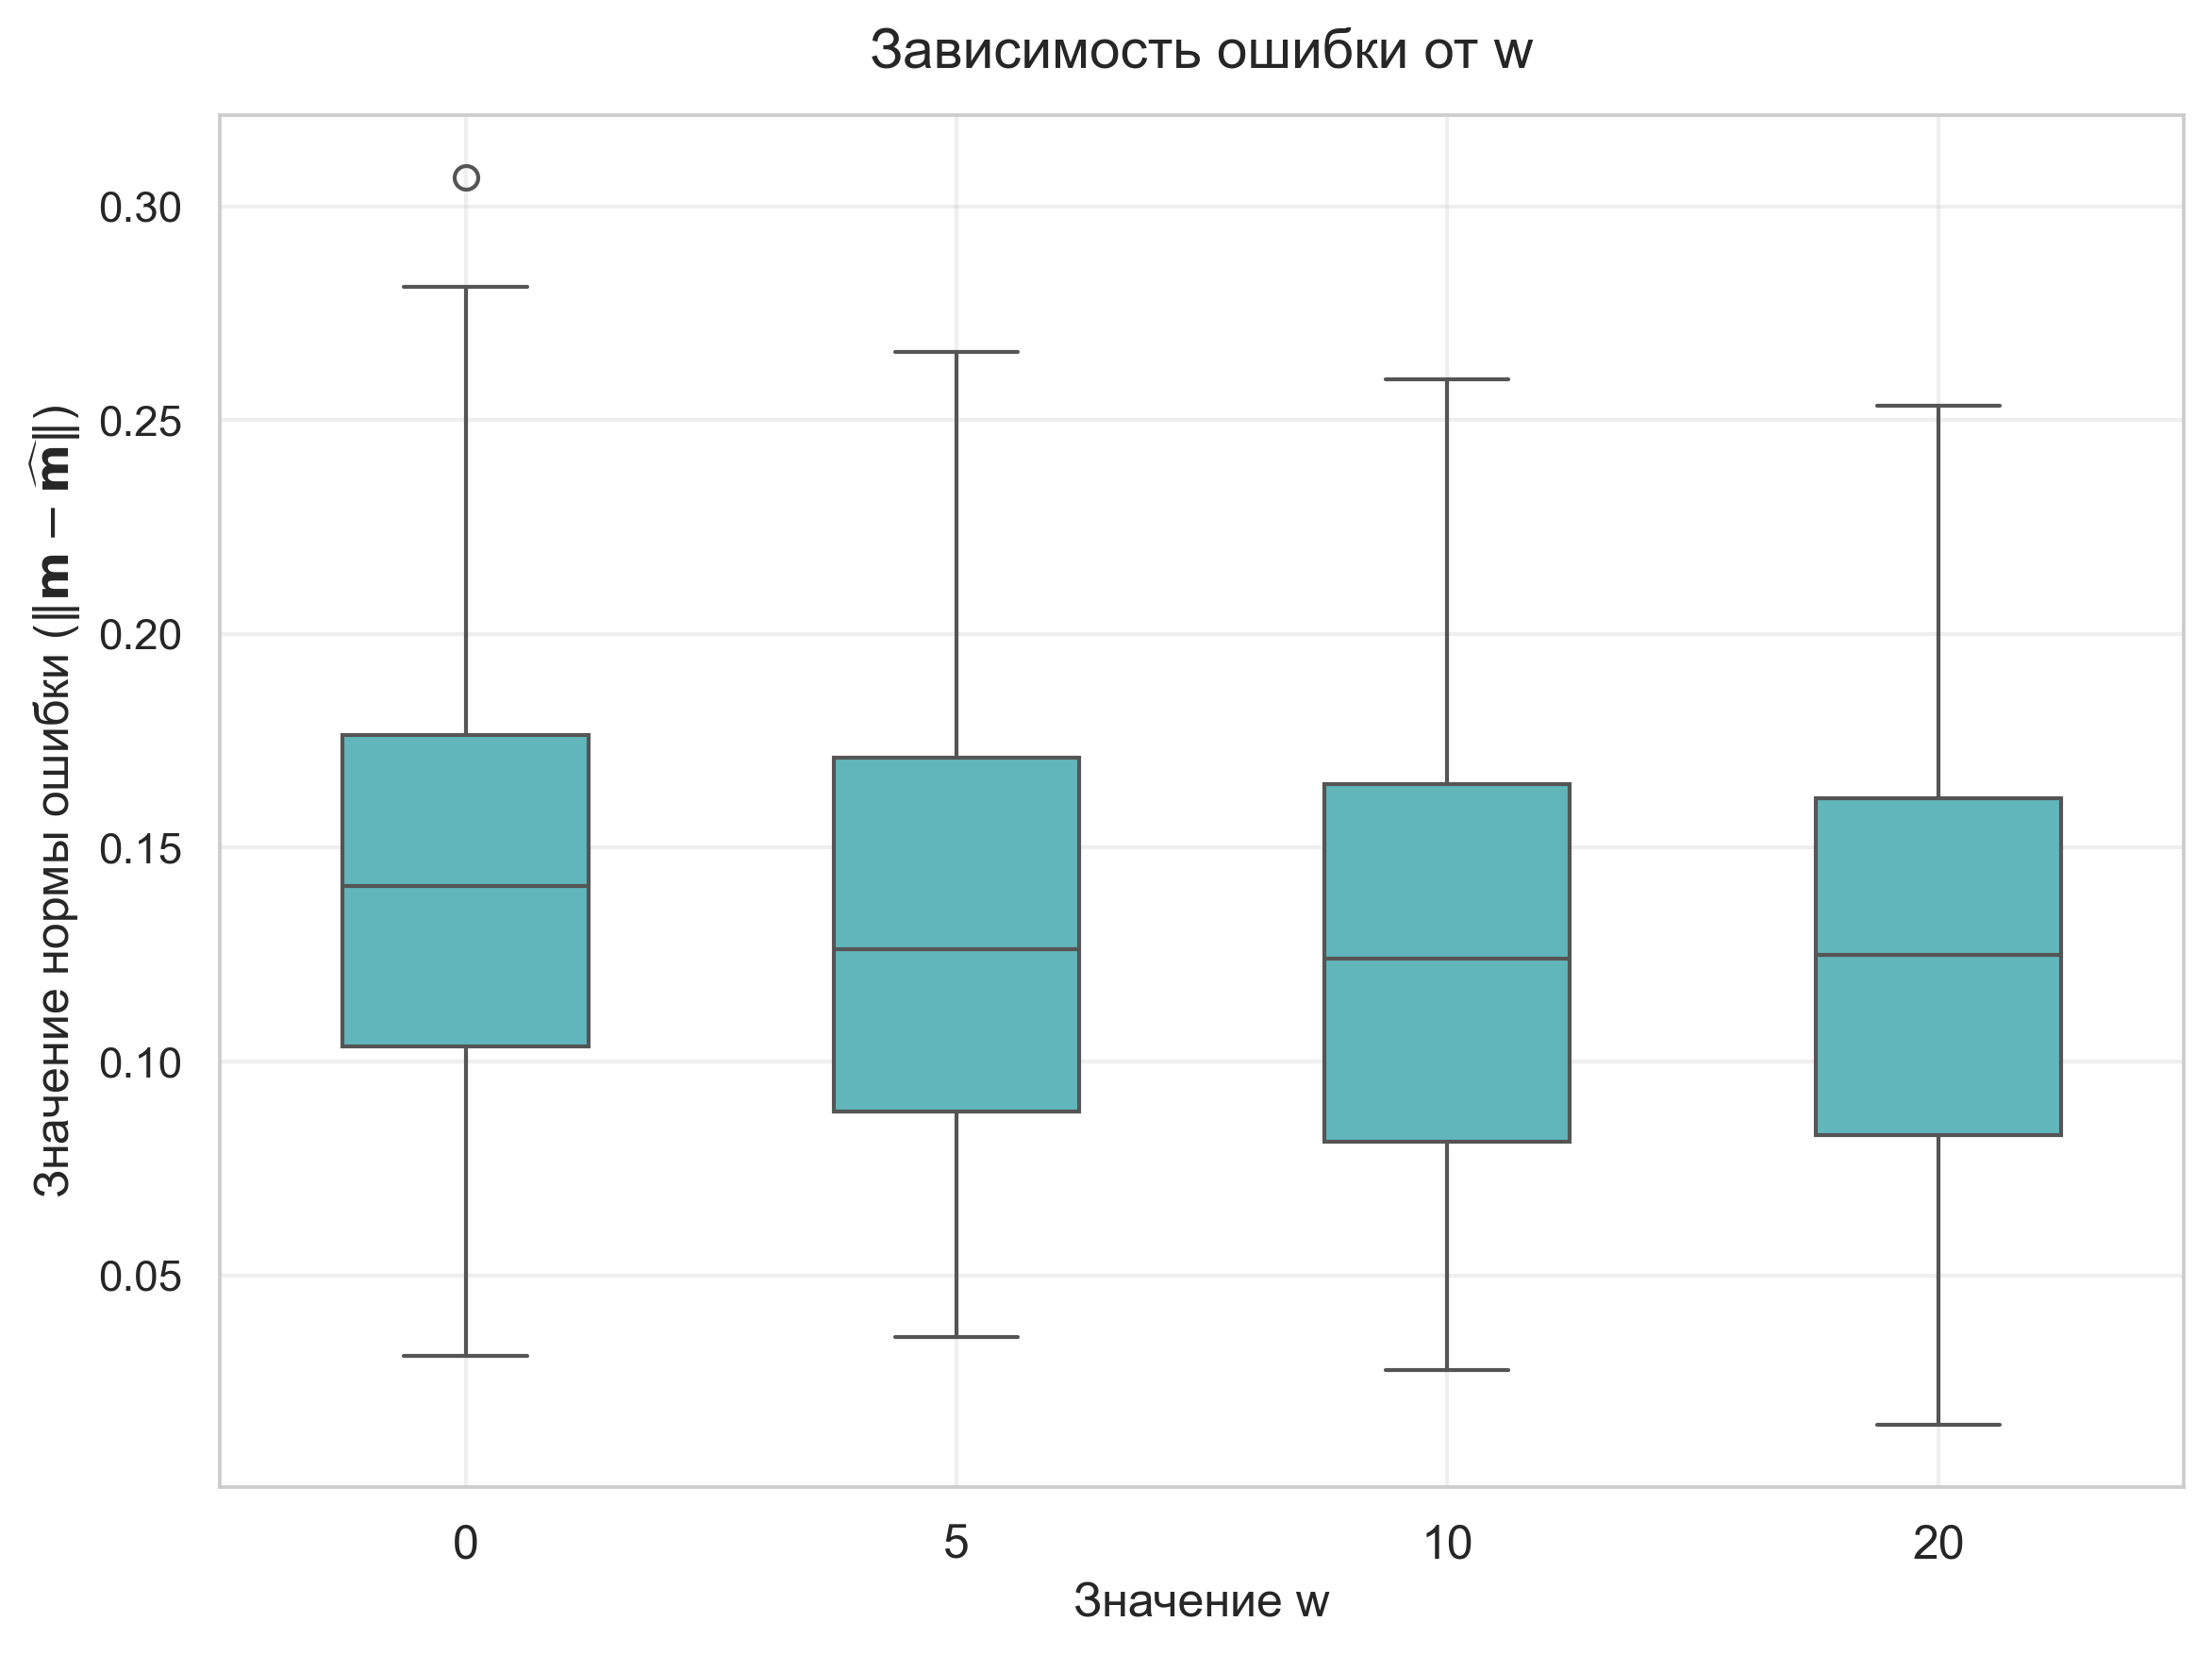
\includegraphics[width=0.8\textwidth]{stochastic_median_additional_steps_boxplots.png}
  \caption{Распределения ошибок модификации алгоритма для различных значений  $\text{w}\in\{0,5,10,20\}$, где ${\text{w}}$ --- число усредняемых последних итераций.}
  \label{fig:additional_steps_boxplots}
\end{figure}

Дальнейшее увеличение параметра ${\text{w}}$ продолжает уменьшать ошибку, однако эффект становится значительно менее выраженным. Таким образом, усреднение последних итераций позволяет повысить точность оценки за счет уменьшения влияния случайных колебаний алгоритма вблизи оптимума.

\subsection{Добавление экспоненциального сглаживания}

Усреднение последних итераций позволяет уменьшить влияние случайных колебаний алгоритма, однако требует выполнения дополнительных итераций уже после достижения критерия останова. Поэтому далее рассмотрим модификацию, изменяющую саму траекторию алгоритма и позволяющую стабилизировать процесс сходимости уже в ходе вычислений.

Для этого предлагается использовать экспоненциальное сглаживание, при котором новое приближение вычисляется как взвешенная комбинация текущей и предыдущей точек траектории.

Пусть последовательность $\widetilde{\mathbf{m}}_i$ задаёт сглаженную траекторию алгоритма, $\widehat{\mathbf{m}}_i$ --- шаг, вычисленный по Алгоритму~\ref{alg:median} из точки $\widetilde{\mathbf{m}}_{i-1}$. Тогда  новое приближение определяется по формуле
\begin{equation}\label{eq:smoothing}
{\widetilde{\mathbf{m}}}_i = \alpha {\widehat{\mathbf{m}}}_i + (1-\alpha) {\widetilde{\mathbf{m}}}_{i-1}, \quad 0 < \alpha \leqslant 1,   
\end{equation}
\vspace{-5ex}

\noindent{где $\alpha$ --- фиксированный параметр сглаживания.} 

Случай $\alpha = 1$ соответствует отсутствию сглаживания. Чем меньше значение $\alpha$, тем сильнее влияние предыдущих приближений на текущую точку траектории.

На Рисунке~\ref{fig:comp_stable_crit_results_exp}  представлены результаты работы алгоритма с экспоненциальным сглаживанием для $\alpha  \in \{0{,}1, \, 0{,}2, \,  0{,}3\}$. Для каждого значения параметра $\alpha$ проводилось моделирование при $c \in\{1,2,\ldots,10\}$, где $c$ --- число  выполнений критерия останова.

Из Рисунка~\ref{fig:comp_stable_crit_results_exp} видно, что использование экспоненциального сглаживания позволяет уменьшить медианное значение ошибки по сравнению с предыдущими модификациями алгоритма.

Для $\alpha=0{,}3$ и $\alpha=0{,}2$ (Рисунки \ref{fig:comp_stable_crit_results_exp_07_03} и \ref{fig:comp_stable_crit_results_exp_08_02}) уменьшение ошибки происходит уже при малых значениях $c$.  Однако дальнейшее увеличение параметра $c$ практически не влияет на распределение ошибок, тогда как число итераций продолжает быстро расти. 

Для $\alpha=0{,}1$ при $\varepsilon=10^{-3}$  (Рисунок \ref{fig:comp_stable_crit_results_exp_09_01}) распределение ошибок становится достаточно <<компактным>> уже при малых значениях $c$, хотя отдельные выбросы все еще сохраняются.  При $\varepsilon=10^{-2}$ разброс ошибок заметно больше, однако постепенно уменьшается при увеличении $c$.

Также видно, что при $\alpha=0{,}1$ рост числа итераций происходит значительно медленнее, чем для больших значений параметра $\alpha$. Таким образом, меньшие значения $\alpha$ позволяют получить более устойчивое распределение ошибок при существенно меньших вычислительных затратах.

Наиболее устойчивые результаты наблюдаются при $\alpha=0{,}1$, $c=5$, $\varepsilon = 10^{-3}$. Для данной комбинации распределение ошибок практически перестает изменяться при дальнейшем увеличении $c$, тогда как вычислительные затраты продолжают расти.

% Анализ результатов показал, что использование $\alpha = 0,3$ и $\alpha =  0,2$ при $c \geqslant 5$ и $\varepsilon = 10^{-3}$ не приводит к существенному улучшению точности по сравнению с $\alpha = 0,1$, но при этом значительно увеличивает вычислительную сложность алгоритма за счет увеличения количества итераций. Однако при $c \leqslant 4$ данные комбинации обеспечивают заметно меньшую ошибку (приблизительно в 2 раза) по сравнению с $\alpha = 0,1$.

% При этом для $\alpha = 0,3$ медианная ошибка не превышает $0,25$ при любом значении $c$ и $\varepsilon$, однако наблюдаются значительные выбросы (максимальная ошибка достигает $2,5$), что не позволяет считать этот вариант оптимальным. Для точности $\varepsilon = 10^{-3}$ и $\alpha = 0,3$ или $\alpha = 0,2$ распределение ошибки стабилизируется, начиная с $c = 2$, но это достигается за счет увеличения количества итераций, что еще раз говорит о том, что данное значение параметра можно не рассматривать и остановить выбор на $\alpha = 0,1$. 

% Для $\alpha = 0,1$ оптимальное значение $c=5$ при точности  $\varepsilon =10^{-3}$, так как при $c > 5$ распределение ошибок практически не изменяется и остается в пределах от 0 до $0,25$. Значение $c = 4$ также можно рассматривать, однако в этом случае наблюдается незначительный выброс по точности.

\begin{figure}[!htbp]
   \centering
\begin{subfigure}[b]{0.99\textwidth}
    \centering
    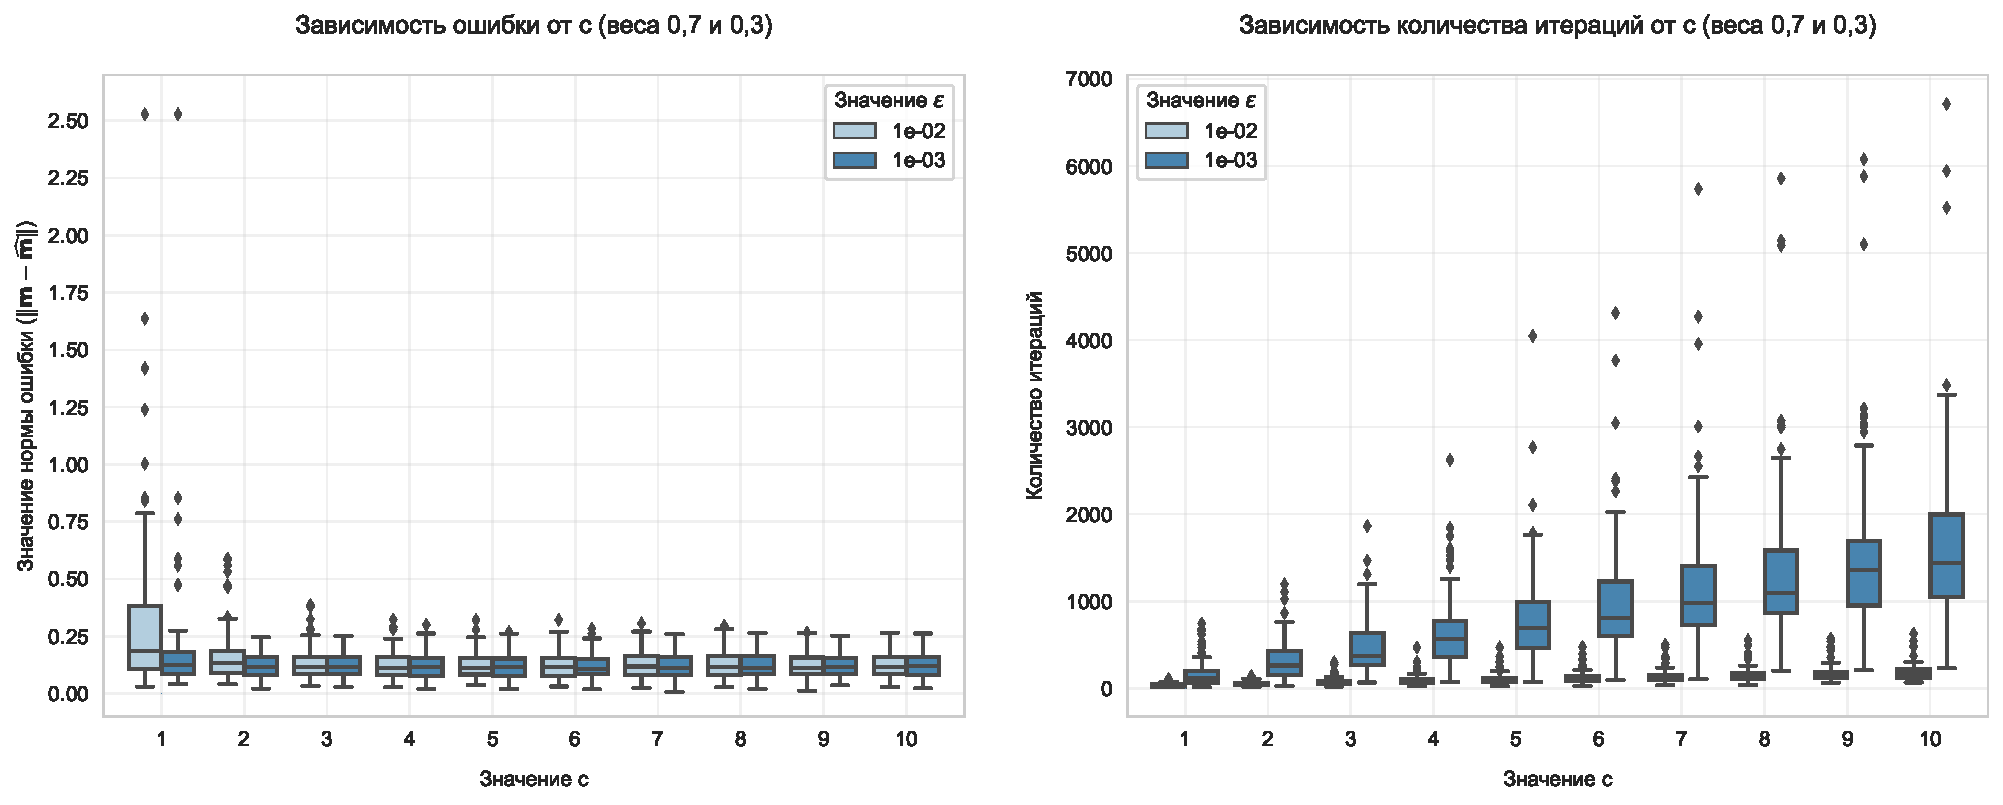
\includegraphics[width=\textwidth]{comp_stable_crit_results_exp_07_03.pdf}
    \captionsetup{labelformat=empty}
     \caption{(а) Распределение числа итераций и нормы ошибки для $\alpha = 0{,}3$}
    \label{fig:comp_stable_crit_results_exp_07_03}
  \end{subfigure}
  
   \vspace{1ex}
    
  \begin{subfigure}[b]{0.99\textwidth}
    \centering
    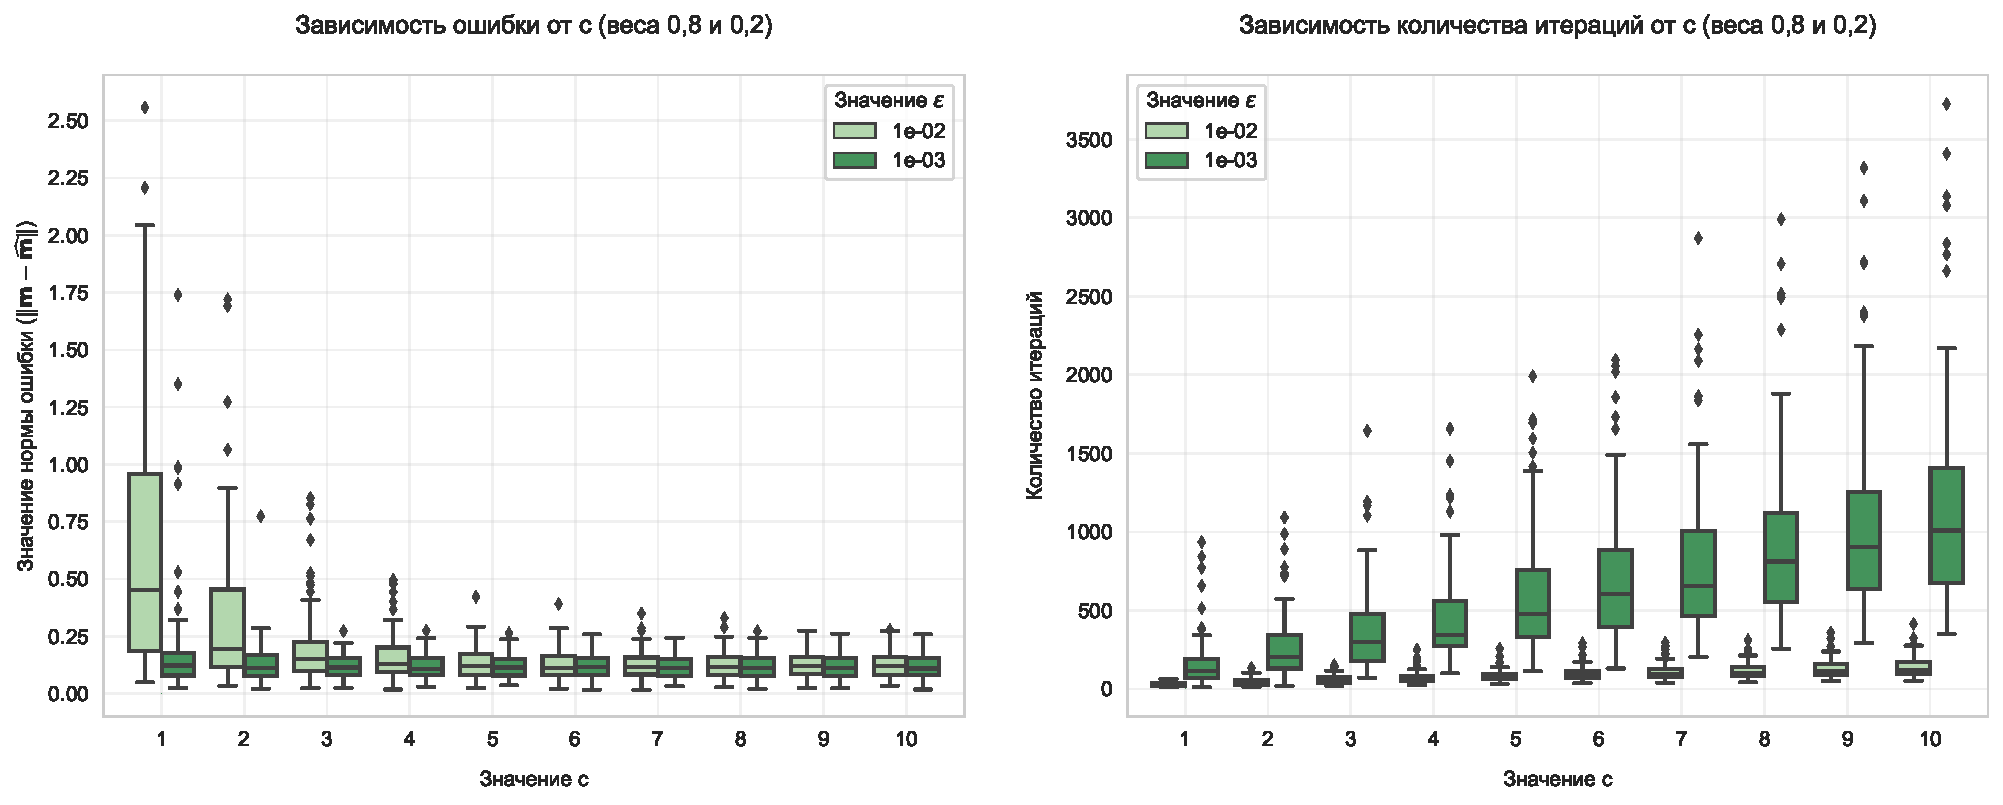
\includegraphics[width=\textwidth]{comp_stable_crit_results_exp_08_02.pdf}
    \captionsetup{labelformat=empty}
      \caption{(б) Распределение числа итераций и нормы ошибки для $\alpha = 0{,}2$}
    \label{fig:comp_stable_crit_results_exp_08_02}
  \end{subfigure}
  
   \vspace{1ex}
      
  \begin{subfigure}[b]{0.99\textwidth}
    \centering
    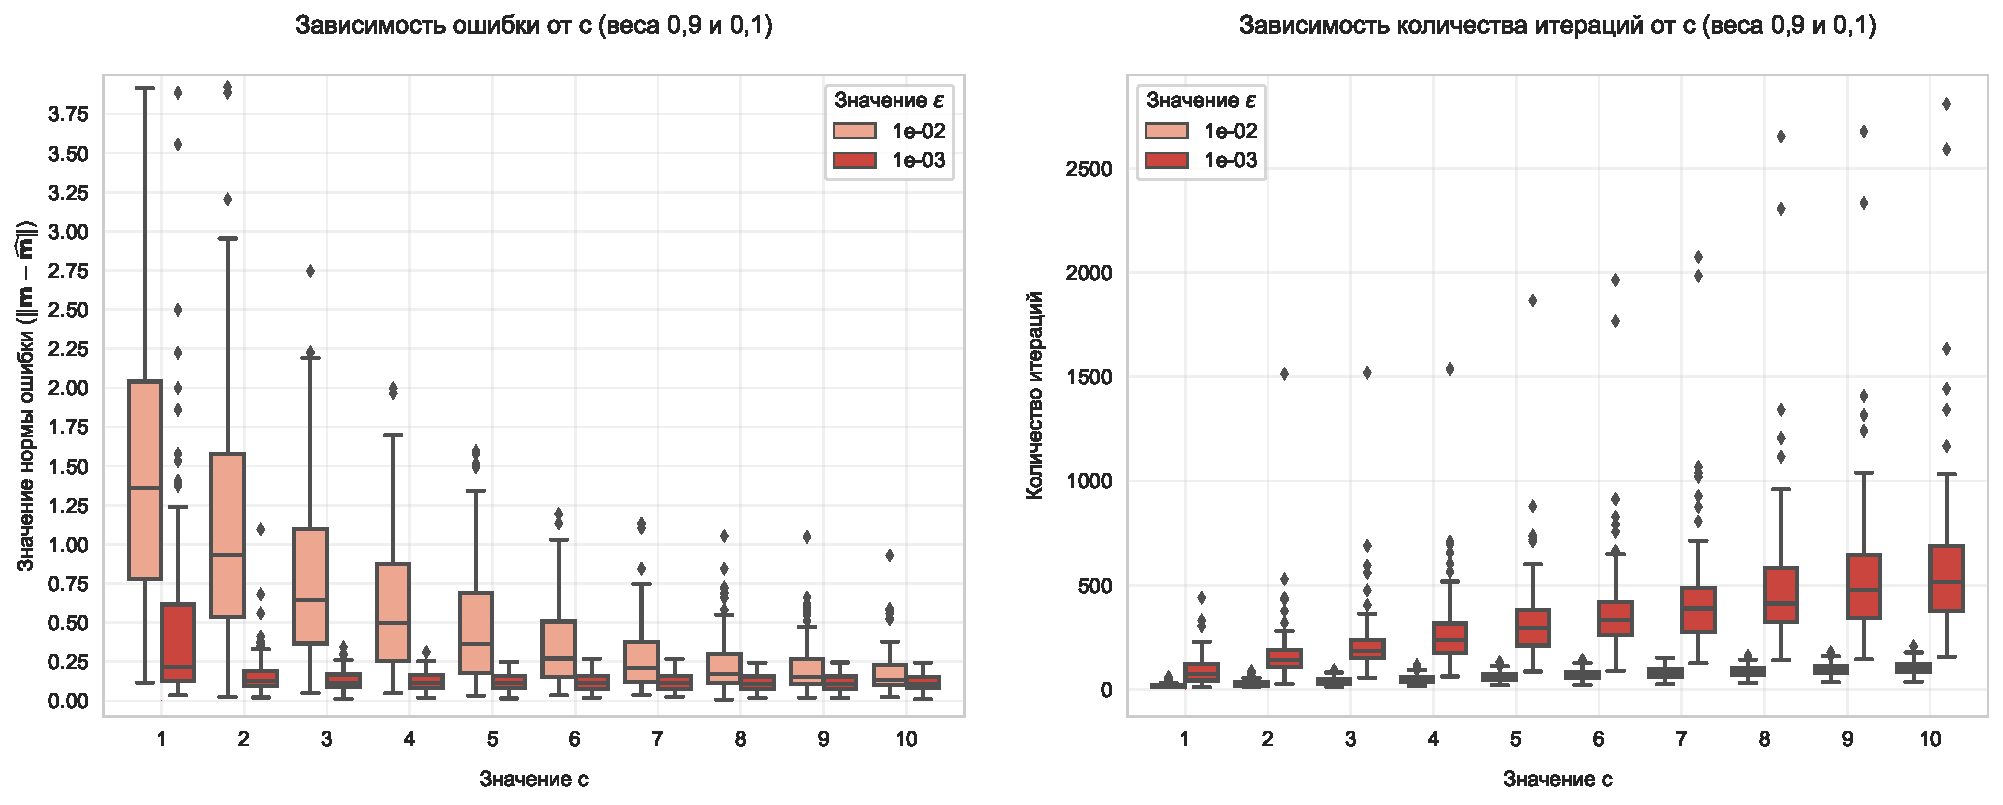
\includegraphics[width=\textwidth]{comp_stable_crit_results_exp_09_01.pdf}
    \captionsetup{labelformat=empty}
      \caption{(в) Распределение числа итераций и нормы ошибки для $\alpha = 0{,}1$}
    \label{fig:comp_stable_crit_results_exp_09_01}
  \end{subfigure}
  \caption{Результаты работы модификации алгоритма с экспоненциальным сглаживанием при различных значениях параметра сглаживания $\alpha$ и числа выполнений критерия останова $c$.
  }
  \label{fig:comp_stable_crit_results_exp}
\end{figure}


На Рисунке~\ref{fig:methods_comparison_exp_vs_avg} приведено сравнение метода с экспоненциальным сглаживанием при $\alpha =  0{,}1$ и $c=5$ (обозначен как  $\text{Exp Stable Rel Crit + Min It}$ на графике) и метода с усреднением последних итераций при ${\text{w}}=20$  с $c=5$  (обозначен как  $\text{Avg Stable Rel Crit + Min It}$ на графике). Видно, что использование экспоненциального сглаживания позволяет получить немного меньшую медианную ошибку и меньший разброс оценок. При этом сопоставимая точность достигается за существенно меньшее число итераций, что делает данный подход более вычислительно эффективным.

\begin{figure}[!htbp]
   \centering
    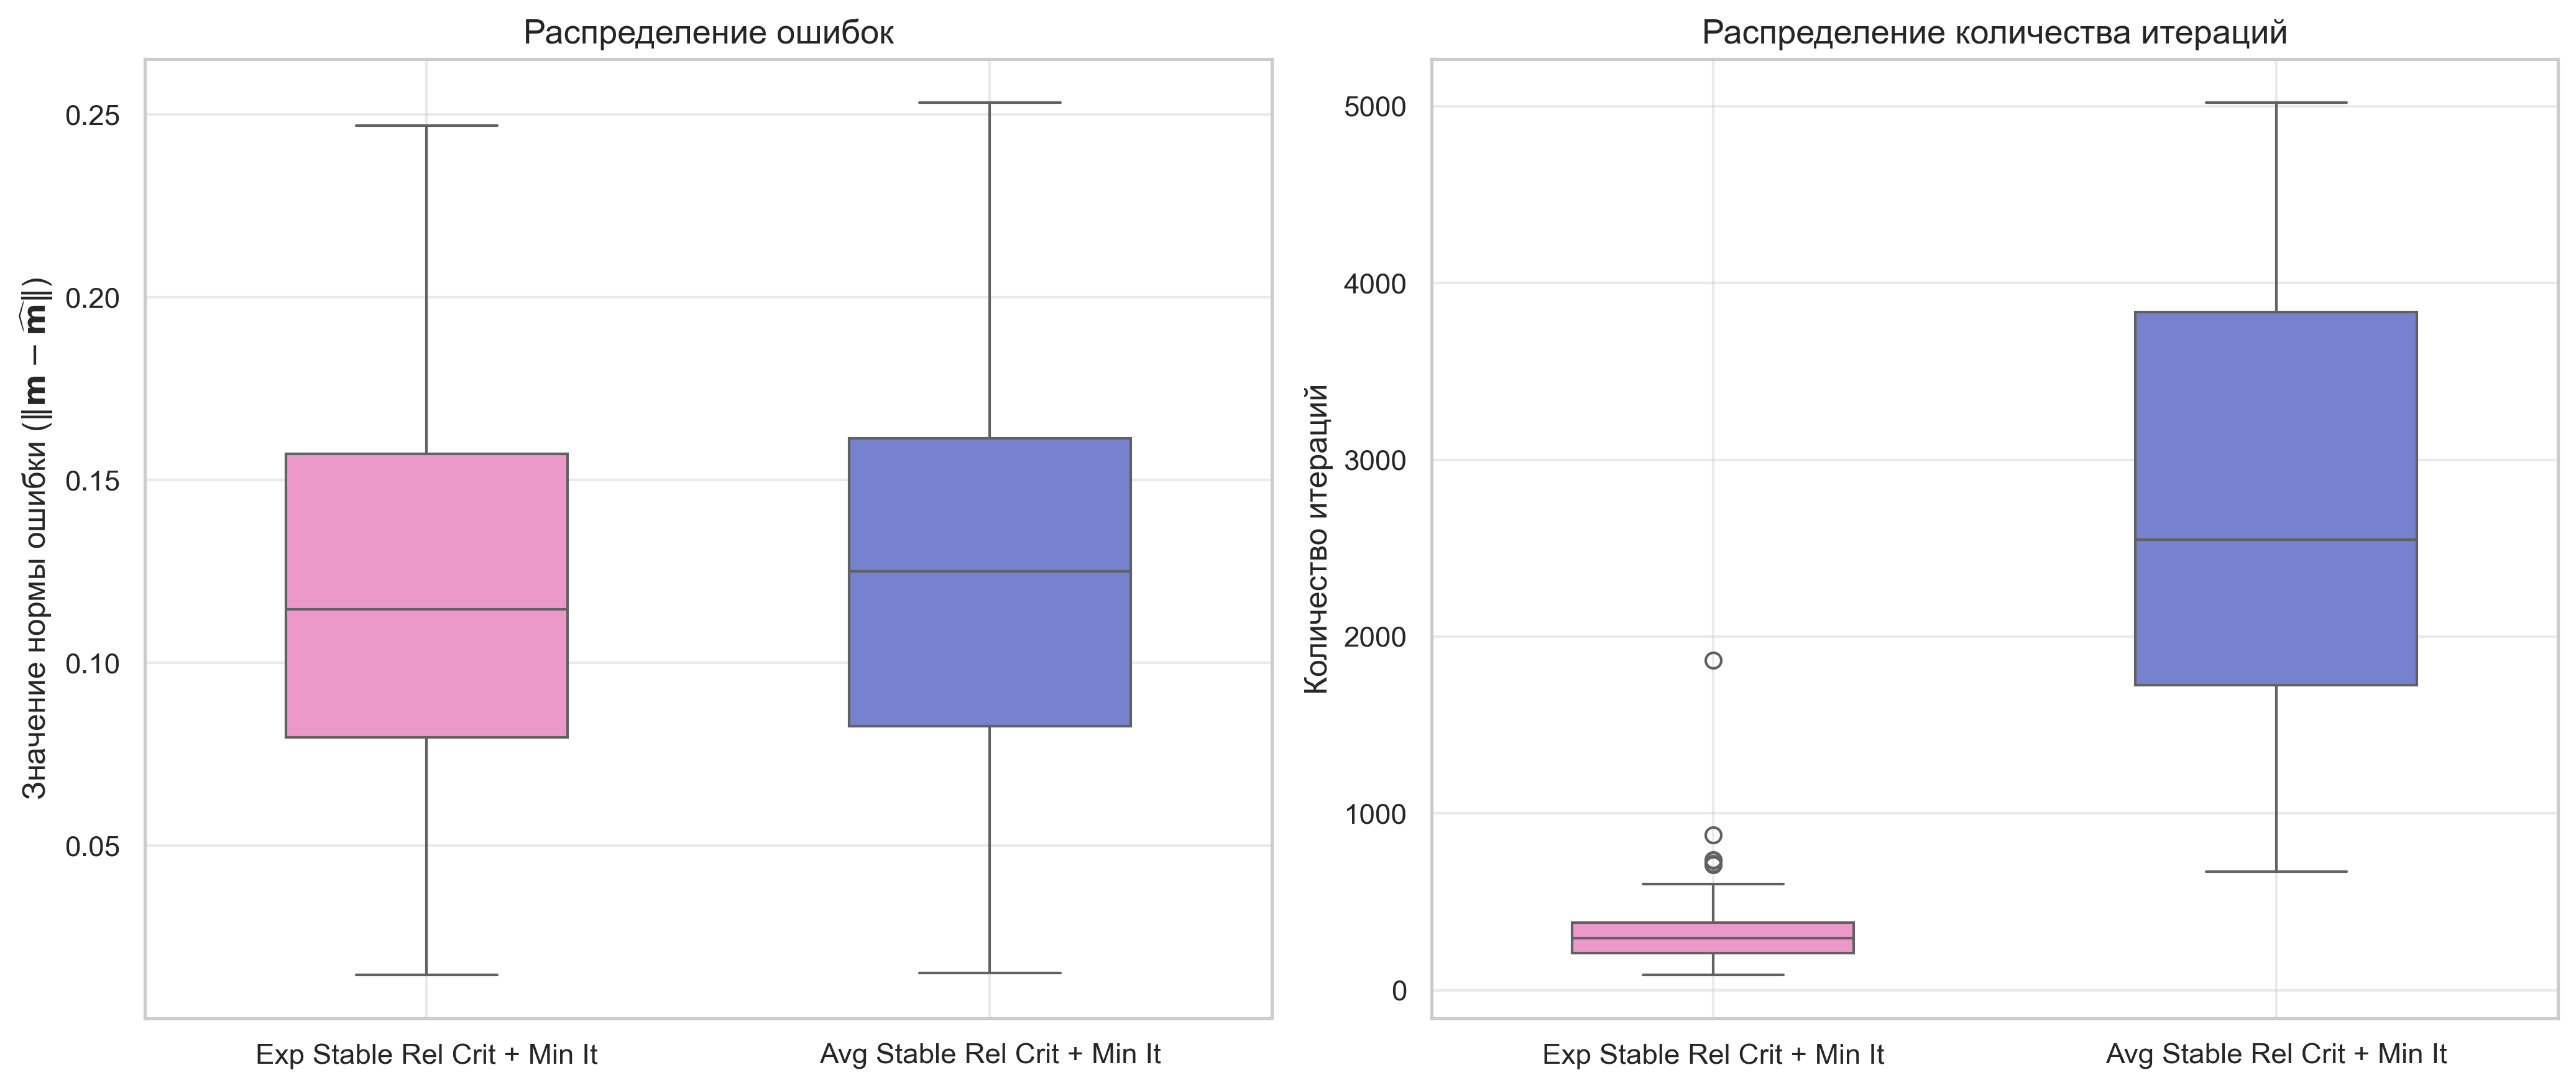
\includegraphics[width=1.01\textwidth]{methods_comparison_exp_vs_avg.png}
  \caption{Сравнение распределений ошибок и количества итераций для метода с усреднением последних итераций и метода с экспоненциальным сглаживанием. }
  \label{fig:methods_comparison_exp_vs_avg}
\end{figure}


\subsection{Применение адаптивного метода выбора шага к предложенному алгоритму}

В данном разделе предлагается посмотреть на предложенный Алгоритм~\ref{alg:median} как на метод, который совершает на итерации шаг вдоль вычисленного направления. Мы доказали в Теореме~\ref{eq:thetheorem}, что Алгоритм~\ref{alg:median} является частным случаем метода стохастического градиента, который, в свою очередь, является методом оптимизации вдоль выбранного направления. Предлагается перенять один подход из теории этих алгоритмов, который улучшает сходимость метода.


\subsubsection{Интерпретация алгоритма как метода оптимизации вдоль направления}

Пусть, как и в случае экспоненциального сглаживания в Алгоритме~\ref{alg:median} с поправкой \eqref{eq:smoothing}, $\widetilde{\mathbf{m}}_i$ обозначает текущее приближение медианы на $i$-й итерации, а $\widehat{\mathbf{m}}_i$ ~--- оценку медианы, полученную в результате проекции выборки на случайное направление, проходящее через $\widetilde{\mathbf{m}}_{i-1}$. Тогда обновление алгоритма можно записать в виде
\begin{equation}\label{eq:improvement_base}
\widetilde{\mathbf{m}}_{i+1} = \widetilde{\mathbf{m}}_i + \gamma_i (\widehat{\mathbf{m}}_{i+1} - \widetilde{\mathbf{m}}_i),
\end{equation}
где $\gamma_i > 0$ --- величина шага на $i$-й итерации. Вектор
\begin{equation}\label{eq:delta}
\delta_i = \widehat{\mathbf{m}}_{i+1} - \widetilde{\mathbf{m}}_i
\end{equation}
можно интерпретировать как направление шага, которое совершает метод. При $\gamma_i = \gamma = 1$ мы получаем стандартный Алгоритм~\ref{alg:median} без сглаживания, а при $\gamma_i = \gamma = \alpha$ из \eqref{eq:smoothing} получаем вариант с экспоненциальным сглаживанием.

Выбор $\alpha$, и, следовательно, $\gamma$ может быть затруднен для конкретной выборки. Предлагается рассмотреть подходы, в которых эта задача решается адаптивно, то есть, $\gamma = \gamma_i$ может меняться с итерацией.% Заметим, что при $\gamma_i = 1$ мы получаем базовый Алгоритм \ref{alg:median}, при $\gamma_i = \alpha$ --- вариант алгоритма с фиксированным экспоненциальным сглаживанием.


\subsubsection{Метод выбора длины шага, подобный AdaGrad}

Метод AdaGrad \cite{duchi2011adaptive} использует покоординатную адаптацию шага на основе накопленной суммы квадратов предыдущих стохастических градиентов. Однако, в контексте итерации~\eqref{eq:improvement_base} обновление принимает вид
\[
G_0 = 0 \in \mathbb{R}^d, \quad G_i = G_{i-1} + \delta_i \odot \delta_i,
\]
\[
\gamma_i = \min\left(1, \frac{\eta}{\sqrt{\sum_{j=1}^d G_j + \varepsilon}}\right),
\]
где $\odot$ обозначает покомпонентное умножение векторов, $\eta$ --- базовая величина шага, а $\varepsilon > 0$~--- малый регуляризационный параметр.

В оригинальной статье \cite{duchi2011adaptive} AdaGrad был введен как метод покомпонентного уточнения длины шага. Проблема в том, что прямое его применение к нашей задаче ухудшает сходимость, так как покомпонентное умножение вектора шага искажает его направление, и, как следствие, оценку параметра положения. Мы рассматриваем модификацию AdaGrad исключительно как метод адаптивного уменьшения длины шага для улучшения сходимости оценки.

\section{Численное сравнение рассмотренных модификаций}

В предыдущих разделах были рассмотрены различные модификации Алгоритма~\ref{alg:median}, направленные на повышение устойчивости и точности оценки. Далее проведем их численное сравнение.

Рассматриваются следующие методы:
\begin{itemize}
    \item алгоритм с относительным критерием останова ($\text{Rel Crit}$);
    
    \item алгоритм с относительным критерием останова и минимальным числом итераций ($\text{Rel Crit + Min It}$);
    
    \item алгоритм с многократным выполнением критерия останова ($\text{Stable Rel Crit}$);
    
    \item алгоритм с многократным выполнением критерия останова и минимальным числом итераций ($\text{Stable Rel Crit + Min It}$);
    
    \item алгоритм с усреднением последних итераций ($\text{Avg Stable Rel Crit + Min It}$);
    
    \item алгоритм с экспоненциальным сглаживанием ($\text{Exp Stable Rel Crit + Min It}$);
    
    \item алгоритм с адаптивным выбором шага на основе AdaGrad с базовым коэффициентом шага $\eta = 10$  ($\text{AdaGrad Stable Rel Crit + Min It}$).
\end{itemize}

Во всех экспериментах выборка объема $n = 1000$ генерировалась из трёхмерного нормального распределения $\mathcal{N}(\mathbf{m}, \mathbf{\Sigma} )$, где вектор математического ожидания $\mathbf{m}$ равен нулю, а в качестве ковариационной матрицы $\mathbf{\Sigma}$ взята матрица \eqref{eq:experimentmatrix}.

Для каждого метода проводилось $200$ независимых запусков алгоритма и рассчитывалась норма ошибки $\|\widehat{\mathbf{m}} - \mathbf{m}\|$, где $\widehat{\mathbf{m}}$ --- оценка медианы, полученная алгоритмом. Параметры у алгоритмов: $\varepsilon = 10^{-3}$, $k_{min}=10$, $c=5$, $\text{w}= 20$.

\vspace{1ex}

Сначала сравним модификации, направленные главным образом на повышение устойчивости алгоритма. Результаты представлены на рисунке~\ref{fig:error_distribution_base_minit_stable}.

\begin{figure}[!htbp]
		\centering
		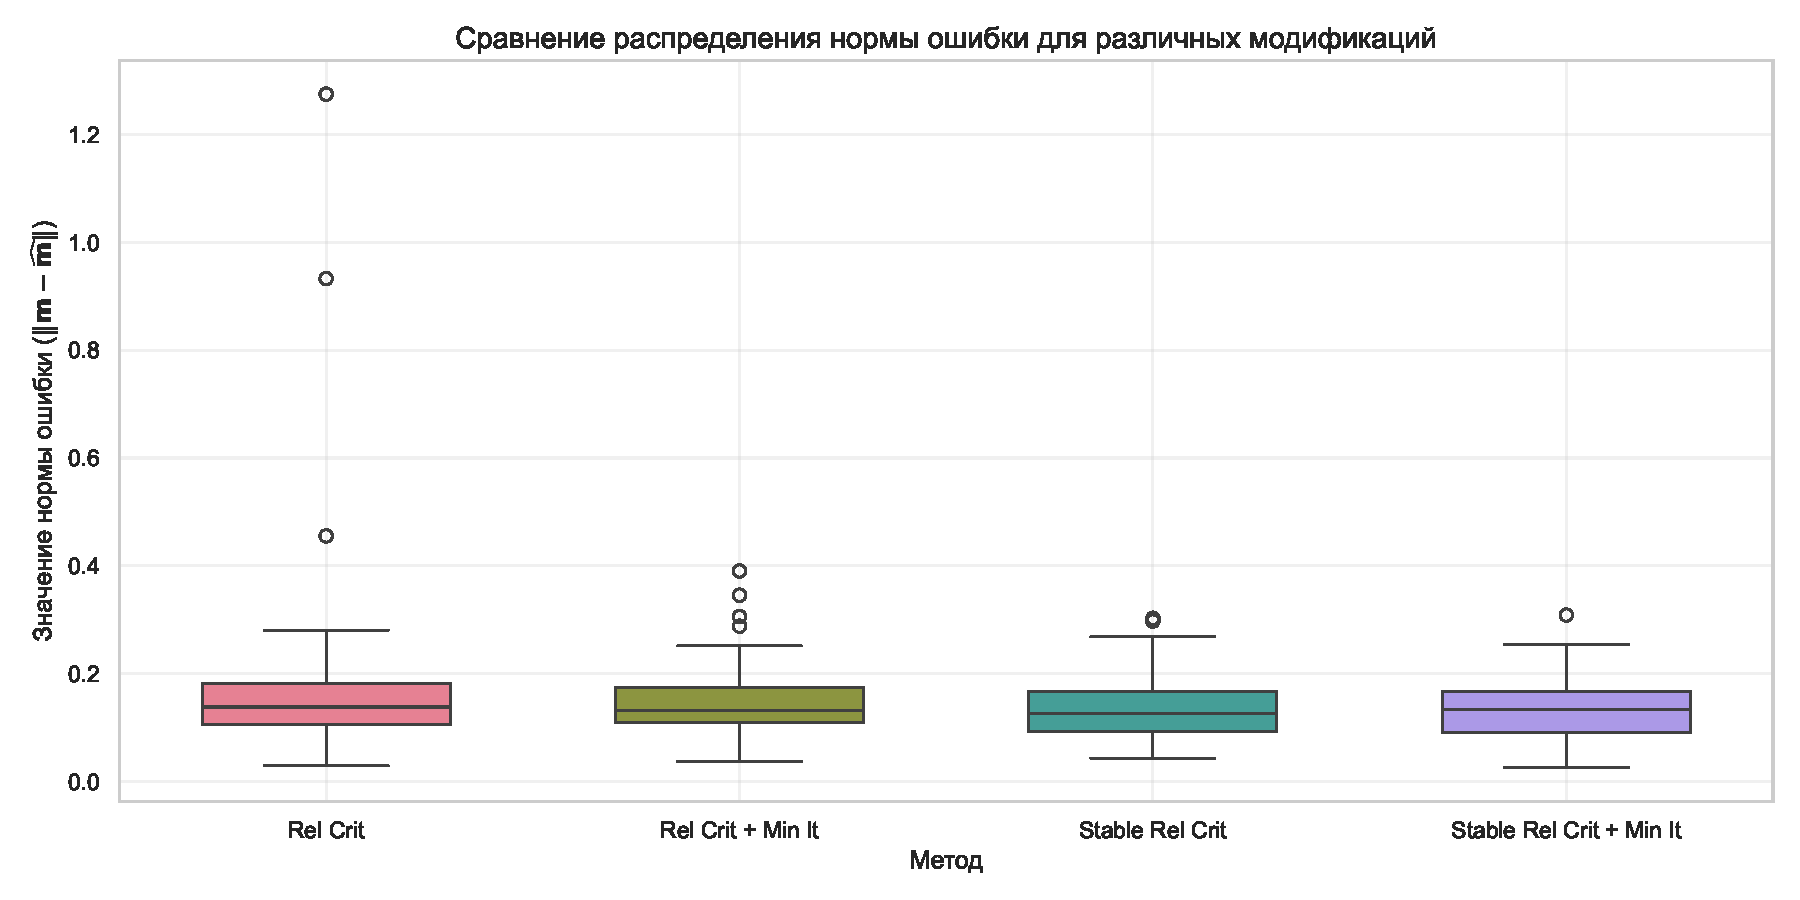
\includegraphics[width=0.9\textwidth]{error_distribution_base_minit_stable.pdf} 
		\caption{Распределения нормы ошибки для модификаций, основанных на изменении критерия останова.}
          \label{fig:error_distribution_base_minit_stable}
\end{figure}

На Рисунке~\ref{fig:error_distribution_base_minit_stable} видно, что использование минимального числа итераций и многократного выполнения критерия останова позволяет существенно уменьшить количество крупных выбросов ошибки по сравнению с алгоритмом, использующим только относительный критерий останова. 

При этом наименьший разброс ошибок наблюдается у метода $\text{Stable Rel Crit}$ + Min It, который сочетает обе модификации одновременно. Таким образом, комбинирование минимального числа итераций и многократного выполнения критерия останова позволяет заметно повысить устойчивость алгоритма.

\vspace{1.5ex}

Далее сравним модификации, изменяющие траекторию алгоритма и направленные непосредственно на повышение точности оценки. Результаты представлены на Рисунке~\ref{fig:error_distribution_ada_exp_avg}. 

\begin{figure}[!htbp]
    \centering
    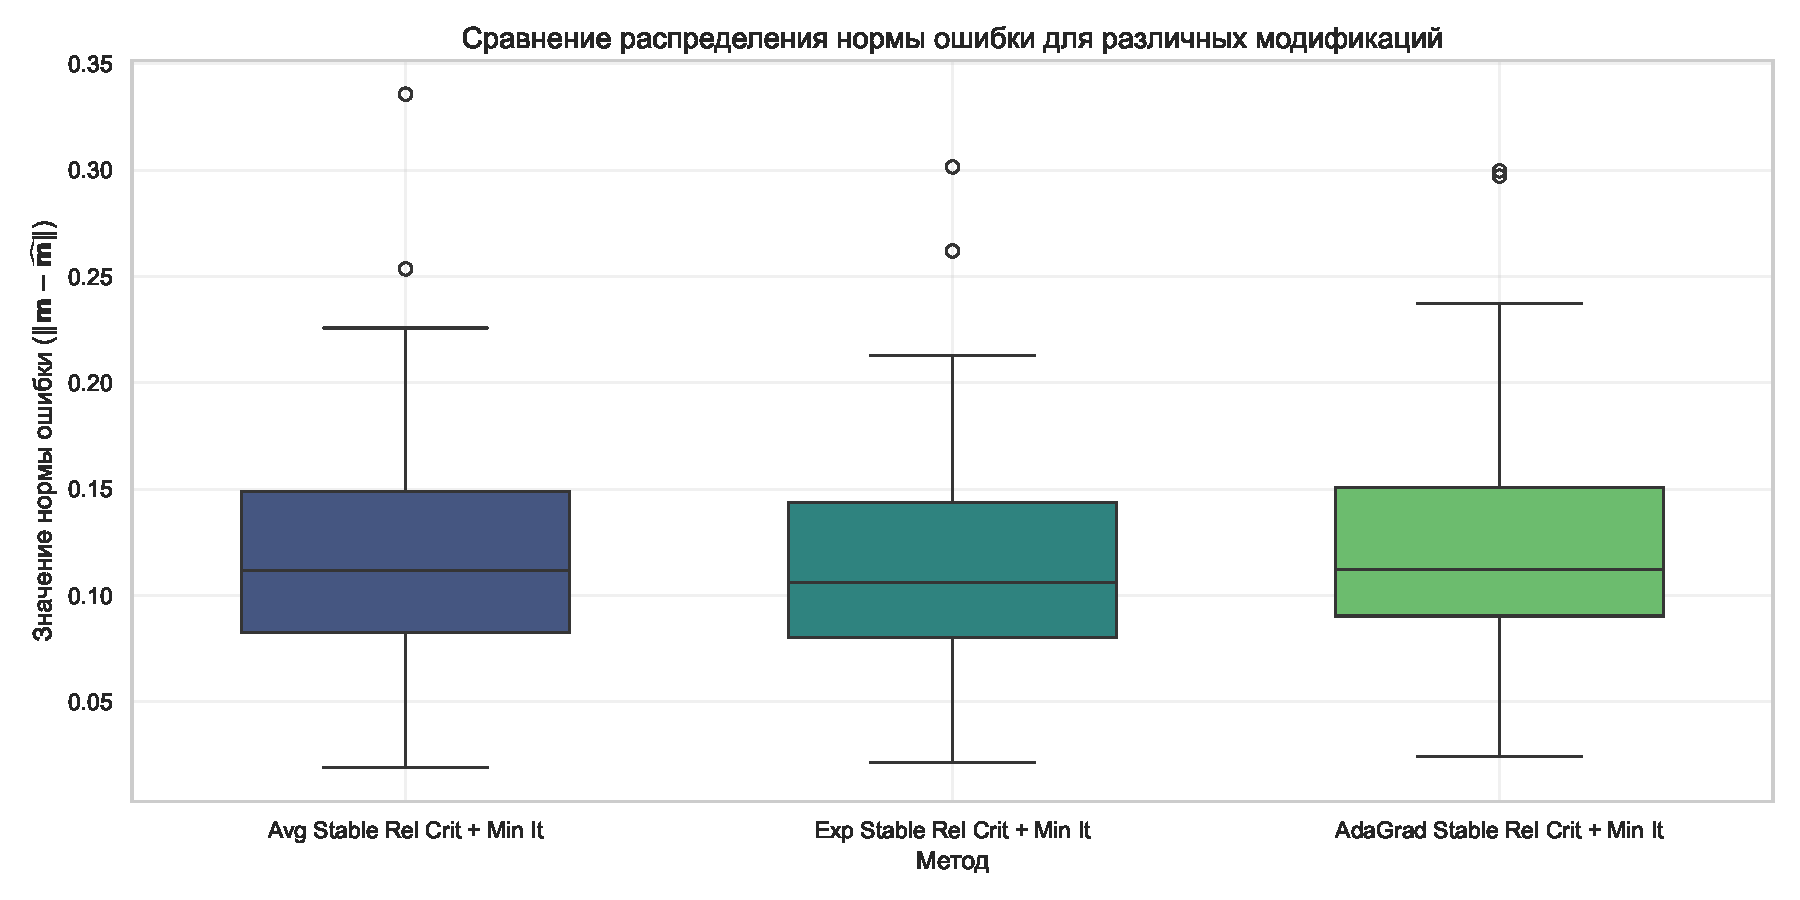
\includegraphics[width=0.9\textwidth]{error_distribution_ada_exp_avg.pdf}
    \caption{Распределения нормы ошибки для модификаций, изменяющих траекторию алгоритма.}
    \label{fig:error_distribution_ada_exp_avg}
\end{figure}

Из Рисунка~\ref{fig:error_distribution_ada_exp_avg} видно, что все три метода демонстрируют близкие результаты. Наибольший разброс ошибок наблюдается у метода с усреднением последних итераций.

Использование экспоненциального сглаживания позволяет немного уменьшить медианное значение ошибки и сделать распределение более компактным. Метод AdaGrad показывает сопоставимые результаты, однако его преимущества перед экспоненциальным сглаживанием оказываются менее выраженными для рассматриваемого распределения.

\vspace{1.5ex}

Наконец, сравним модификации, изменяющие траекторию алгоритма, с предыдущими модификациями критерия останова. Результаты представлены на Рисунке~\ref{fig:error_distribution_not_base}. 

% На Рисунке~\ref{fig:error_distribution_ada_exp_avg} представлены боксплоты распределений ошибок для всех рассматриваемых методов.

\begin{figure}[!htbp]
    \centering
    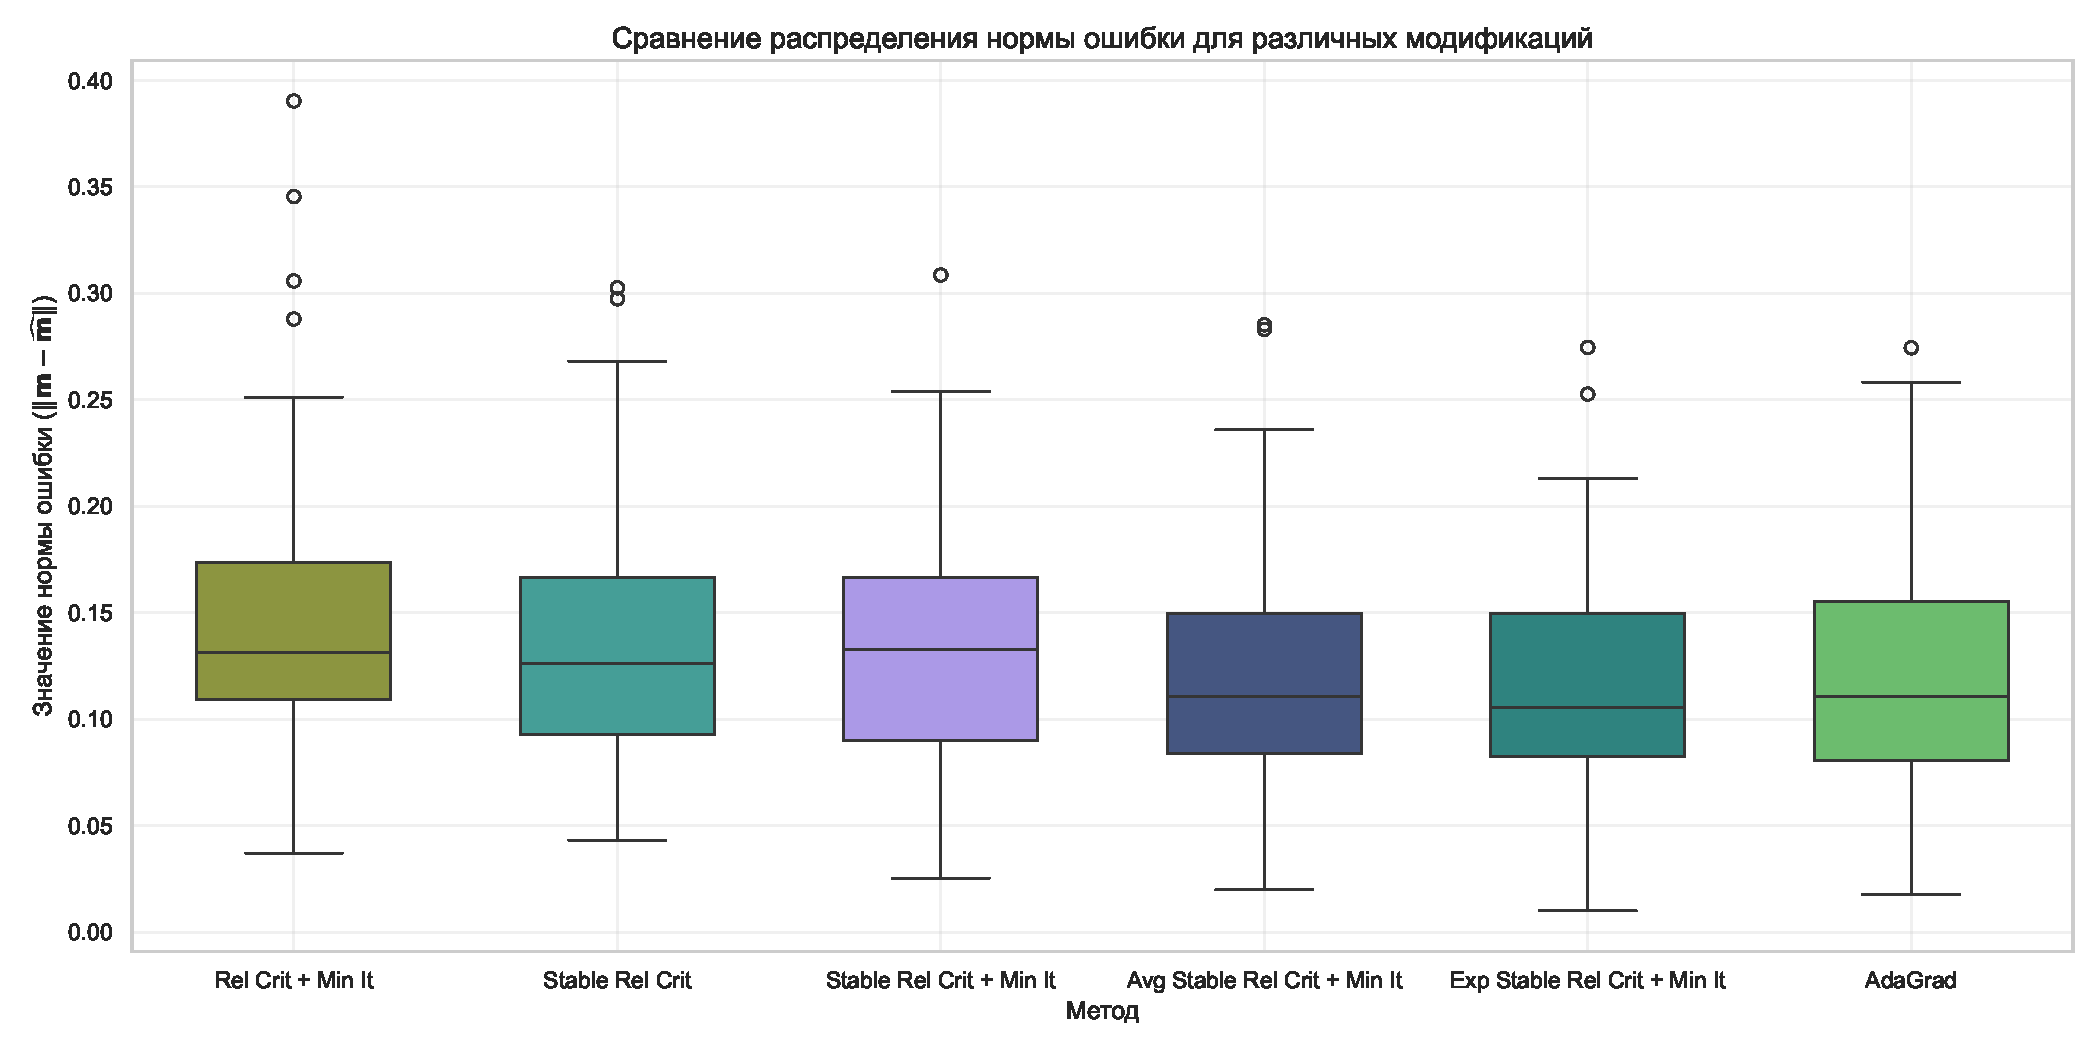
\includegraphics[width=0.9\textwidth]{error_distribution_not_base.pdf}
    \caption{Сравнение распределений нормы ошибки для различных модификаций алгоритма.}
    \label{fig:error_distribution_not_base}
\end{figure}


Из Рисунка~\ref{fig:error_distribution_not_base} видно, что модификации, изменяющие траекторию алгоритма, позволяют дополнительно уменьшить медианное значение ошибки по сравнению с методами, основанными только на изменении критерия останова.

Наиболее устойчивые результаты демонстрируют методы $\text{Exp Stable Rel Crit}$ + Min It и $\text{AdaGrad Stable Rel Crit + Min It}$. При этом метод с экспоненциальным сглаживанием показывает немного меньший разброс ошибок.

Таким образом, модификации траектории оказываются более эффективными для повышения точности оценки, чем модификации, связанные исключительно с критерием останова. В то же время методы, основанные на изменении критерия останова, существенно повышают устойчивость алгоритма и уменьшают вероятность появления крупных ошибок.


\section{Исследование робастности модификаций алгоритма}

Помимо точности и устойчивости алгоритма, важным свойством рассматриваемых методов является робастность. В работе~\cite{filatova2024robust} было показано, что базовый Алгоритм~\ref{alg:median} устойчив к наличию выбросов. Однако добавление модификаций, изменяющих критерий останова и траекторию сходимости, может влиять на данное свойство. Поэтому далее исследуется, как различные модификации алгоритма ведут себя при увеличении доли выбросов в выборке.

Во всех экспериментах использовались те же данные, что и в предыдущем разделе: выборки объема $n=1000$ генерировались из трехмерного нормального распределения с $\mathbf{m}=\mathbf{0}$ и ковариационной матрицей \eqref{eq:experimentmatrix}.

Для исследования робастности часть наблюдений в выборке заменялась на точку-выброс $(100; 100; 100)^{\mathrm T}$ с весом $\{0\%,\,5\%,\,10\%,\,15\%,\,20\%,\,25\%\}.$

Для каждого метода проводилось $200$ независимых запусков алгоритма и рассчитывалась норма ошибки $\|\widehat{\mathbf{m}} - \mathbf{m}\|$, где $\widehat{\mathbf{m}}$ --- оценка параметра положения, полученная алгоритмом.

В сравнение также была включена геометрическая медиана, поскольку, как отмечалось ранее, именно она является основным конкурентом предложенного алгоритма с точки зрения точности и вычислительной эффективности.

На Рисунке~\ref{fig:location_error_dependency} представлена зависимость средней ошибки оценки параметра положения от веса точки-выброса для различных модификаций алгоритма.

\begin{figure}[!htbp]
    \centering
    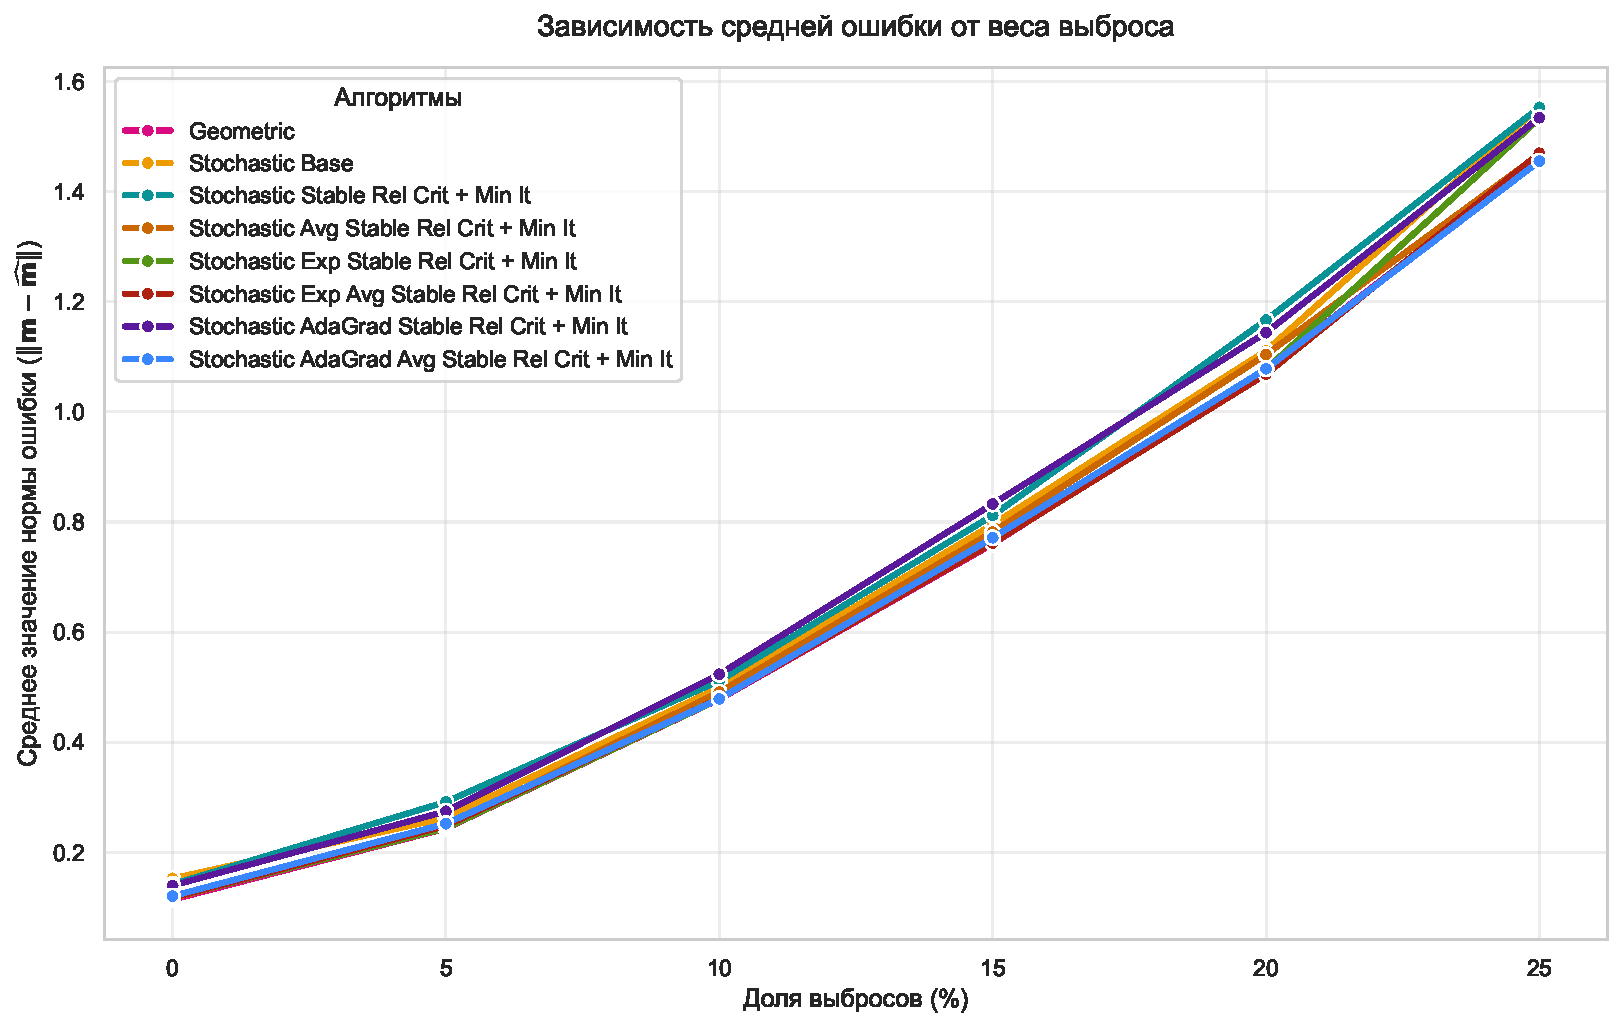
\includegraphics[width=0.9\textwidth]{location_error_dependency.pdf}
    \caption{Зависимость средней нормы ошибки от веса точки-выброса для различных модификаций алгоритма.}
    \label{fig:location_error_dependency}
\end{figure}

Из Рисунка~\ref{fig:location_error_dependency} видно, что для всех рассматриваемых методов ошибка монотонно возрастает с увеличением веса выброса. Однако различия между алгоритмами оказываются сравнительно небольшими.

Геометрическая медиана заметно не выделяется на этом графике, что говорит о том, что предложенный алгоритм сопаставим с ней по свойствам робасности.

Среди модификаций стохастического алгоритма наиболее устойчивые результаты показывают методы, использующие усреднение и сглаживание траектории. В частности, модификации Stochastic Exp Avg Stable Rel Crit и Stochastic AdaGrad Avg Stable Rel Crit демонстрируют немного меньшие значения ошибки по сравнению с базовыми версиями алгоритма. Тем не менее различия между методами остаются относительно небольшими даже при $20\%-25\%$ выбросов.

В целом эксперимент показывает, что предложенные модификации позволяют сохранить робастные свойства алгоритма при наличии выбросов, а использование сглаживания и усреднения траектории позволяет дополнительно уменьшить ошибку оценки параметра положения.


% \section{Рассмотрение случаев, когда алгоритм не сходится}

% На рисунке~\ref{fig:V_comp} изображены результаты работы известных алгоритмов по оценке многомерной медианы (Оджа, Тьюки и геометрическая), а также результаты 200 запусков предложенного алгоритма в следующих вариациях: с использованием относительного критерия (рис.~\ref{fig:V_rel}), с использованием относительного критерия и усреднением по последним 20 итерациям  (рис.~\ref{fig:V_rel_avg}), с экспоненциальным сглаживанием с $\alpha = 0,1$ и $c=5$ (рис.~\ref{fig:V_exp}), а также с экспоненциальным сглаживанием при тех же условиях и  усреднением по последним 20 итерациям (рис.~\ref{fig:V_exp_avg}). 

% На основе данных графиков можно заметить, что алгоритмы оценки медиан Тьюки, Оджа и геометрической сходятся примерно в одну точку, в то время как базовая версия (рис.~\ref{fig:V_rel}) предложенного алгоритма демонстрирует значительный разброс оценок, формируя хаотичное облако точек. Если же добавить усреднение по последним итерациям  (рис.~\ref{fig:V_rel_avg}), то разброс уже не такой выраженный и полученные оценки образуют более однородное и компактное облако. 


% Применение экспоненциального сглаживания приводит к еще большему уменьшению разброса (рис.~\ref{fig:V_exp}), размеры облака становятся заметно меньше. Если же еще добавить усреднение (рис.~\ref{fig:V_exp_avg}), то результаты хоть и незначительно, но все же еще улучшатся и разброс значений по оси y не будет превышать $0,1$, что является существенным улучшением по сравнению с исходной ситуацией. 


% \begin{figure}[h]
%   \centering
%   \begin{subfigure}[b]{0.4\textwidth}
%     \centering
%     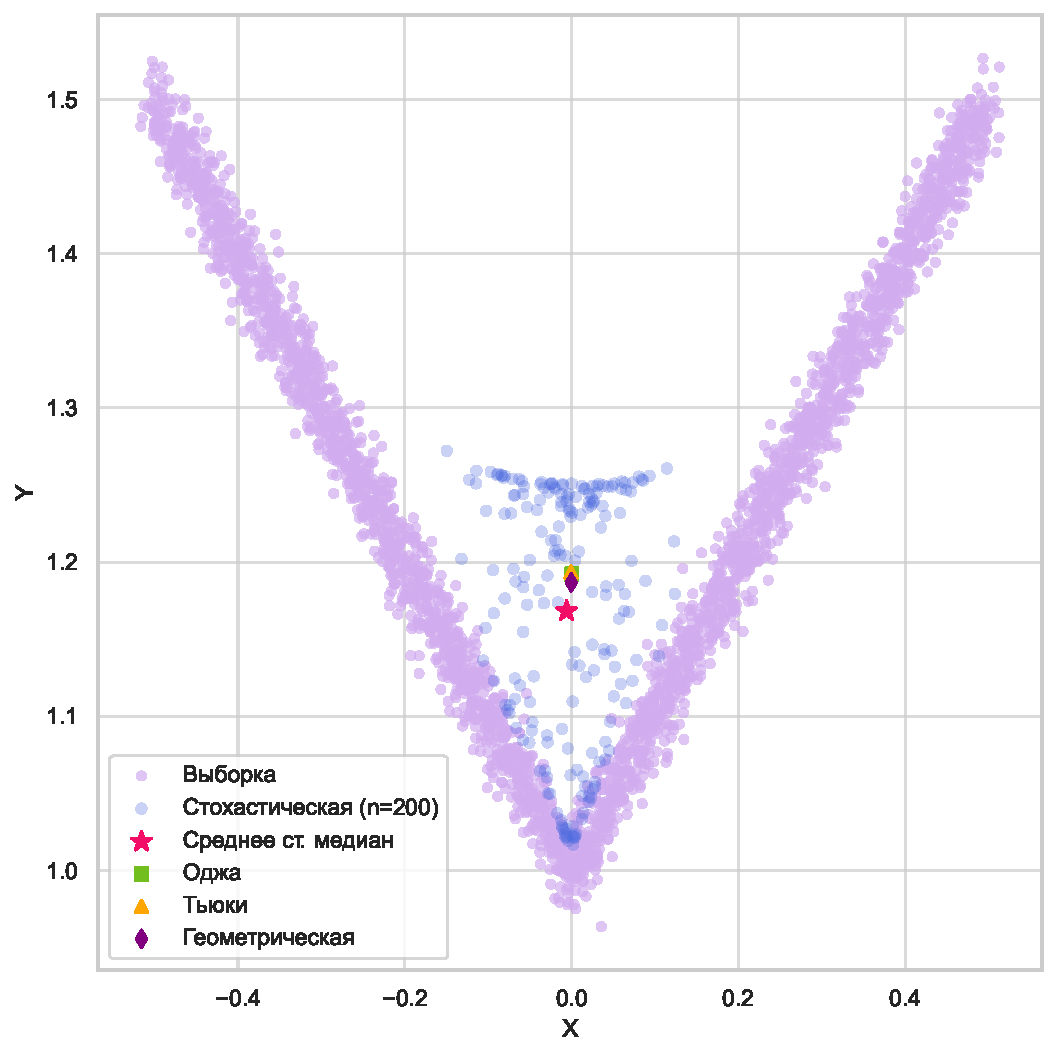
\includegraphics[width=\textwidth]{sample_V_base.pdf}
%     \captionsetup{labelformat=empty}
%      \caption{(a) Base}
%      \label{fig:V_rel}
%   \end{subfigure}
%   \begin{subfigure}[b]{0.4\textwidth}
%     \centering
%     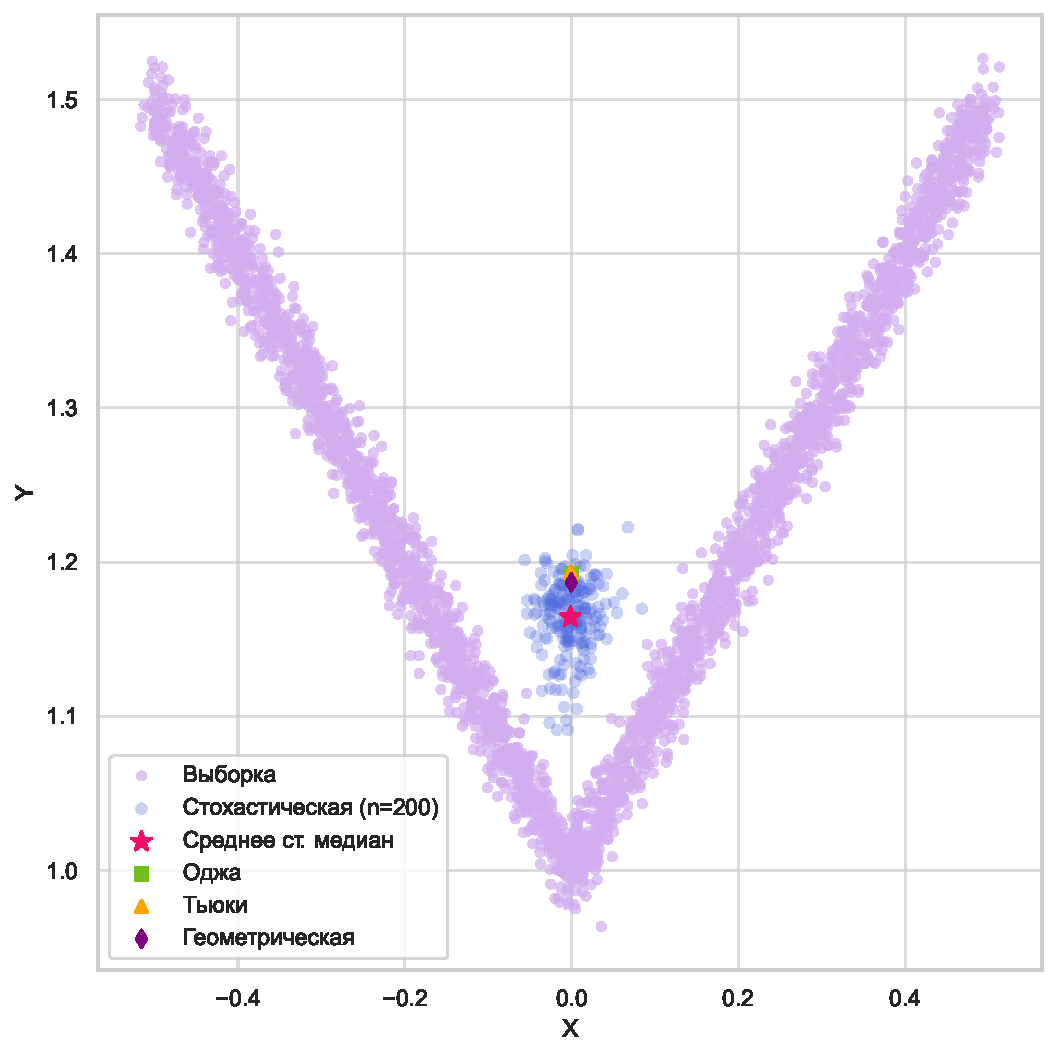
\includegraphics[width=\textwidth]{sample_V_base_avg.pdf}
%     \captionsetup{labelformat=empty}
%     \caption{(d) Base + Avg}
%    \label{fig:V_rel_avg}
%   \end{subfigure}
%   \begin{subfigure}[b]{0.4\textwidth}
%     \centering
%     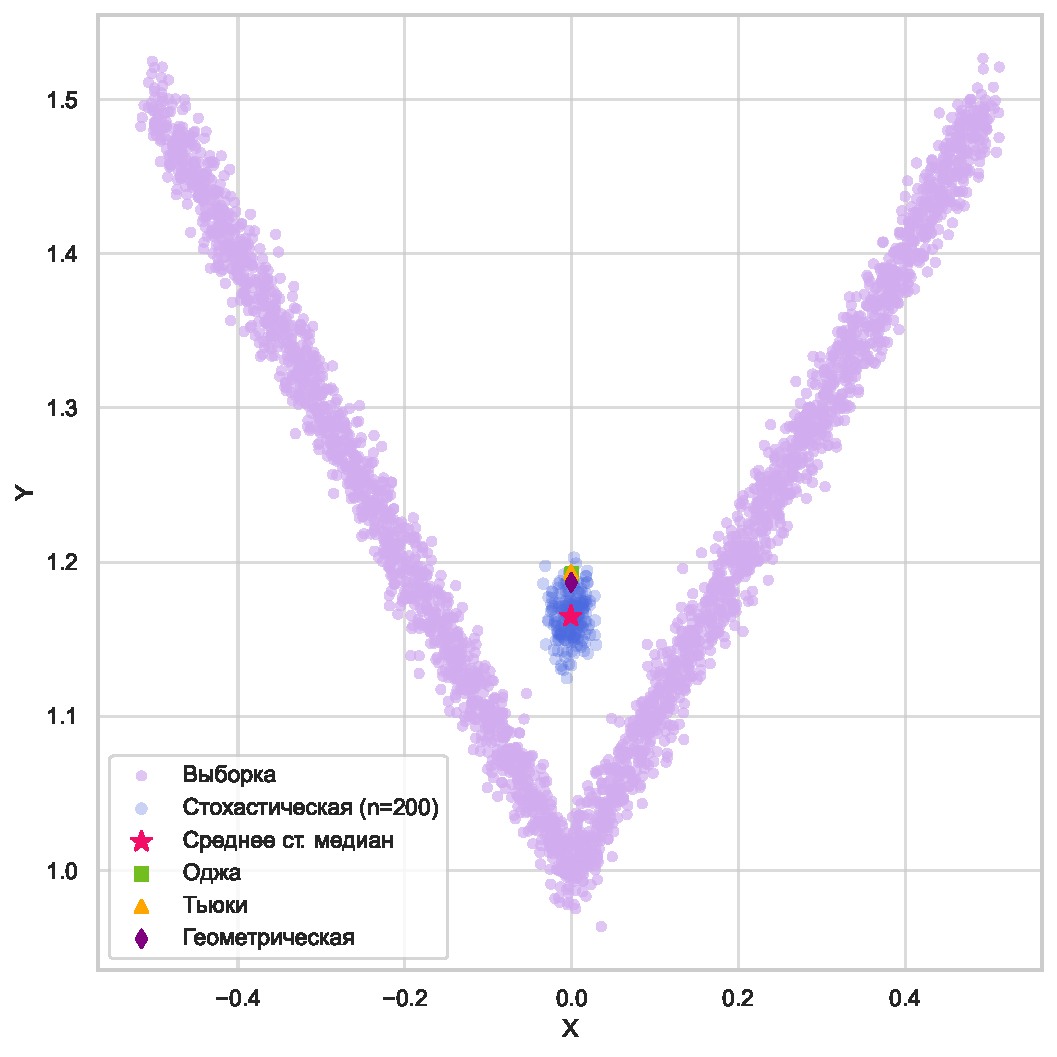
\includegraphics[width=\textwidth]{sample_V_exp.pdf}
%     \captionsetup{labelformat=empty}
%      \caption{Exp}
%      \label{fig:V_rel_exp}
%   \end{subfigure}
%   \centering
%   \begin{subfigure}[b]{0.4\textwidth}
%     \centering
%     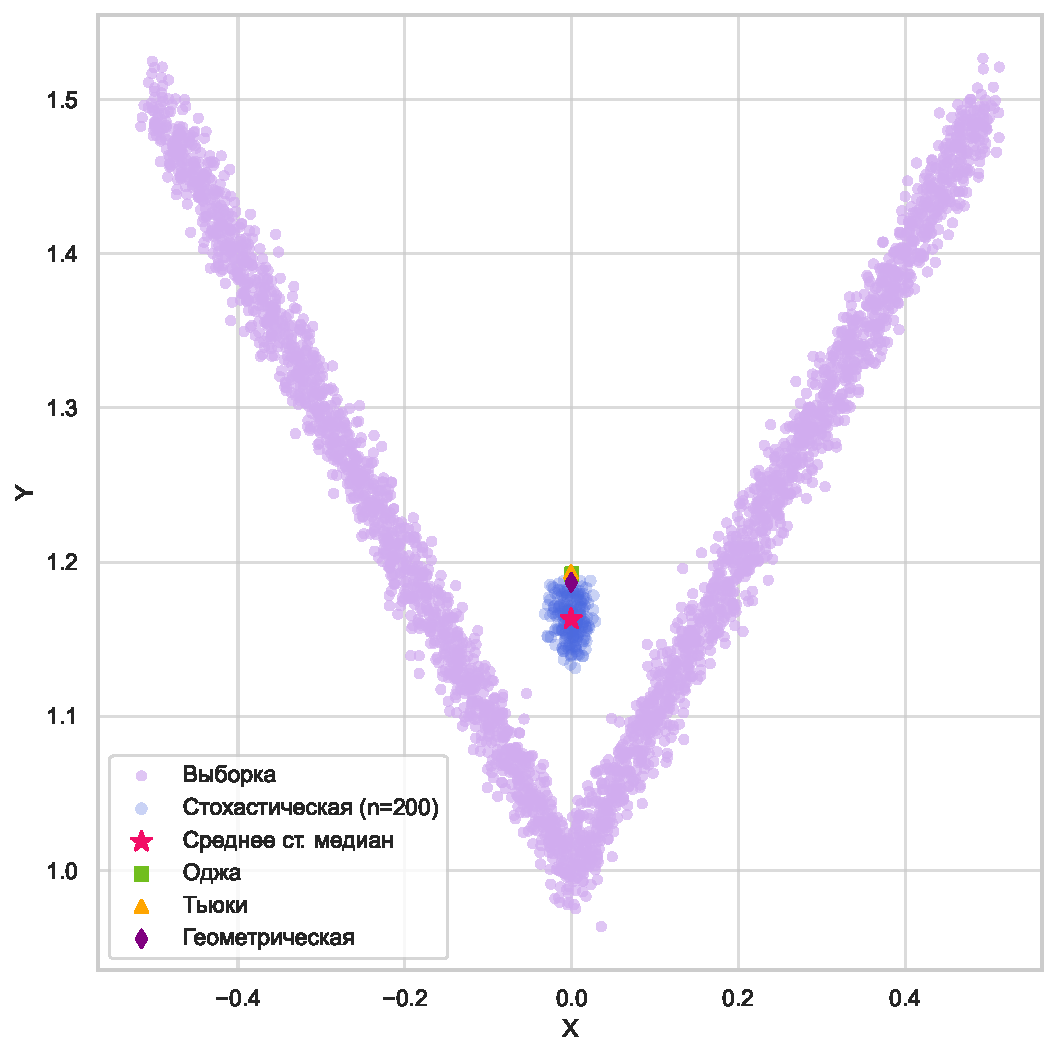
\includegraphics[width=\textwidth]{sample_V_exp_avg.pdf}
%     \captionsetup{labelformat=empty}
%      \caption{Exp + Avg}
%      \label{fig:V_rel_exp_avg}
%   \end{subfigure}
%   \begin{subfigure}[b]{0.4\textwidth}
%     \centering
%     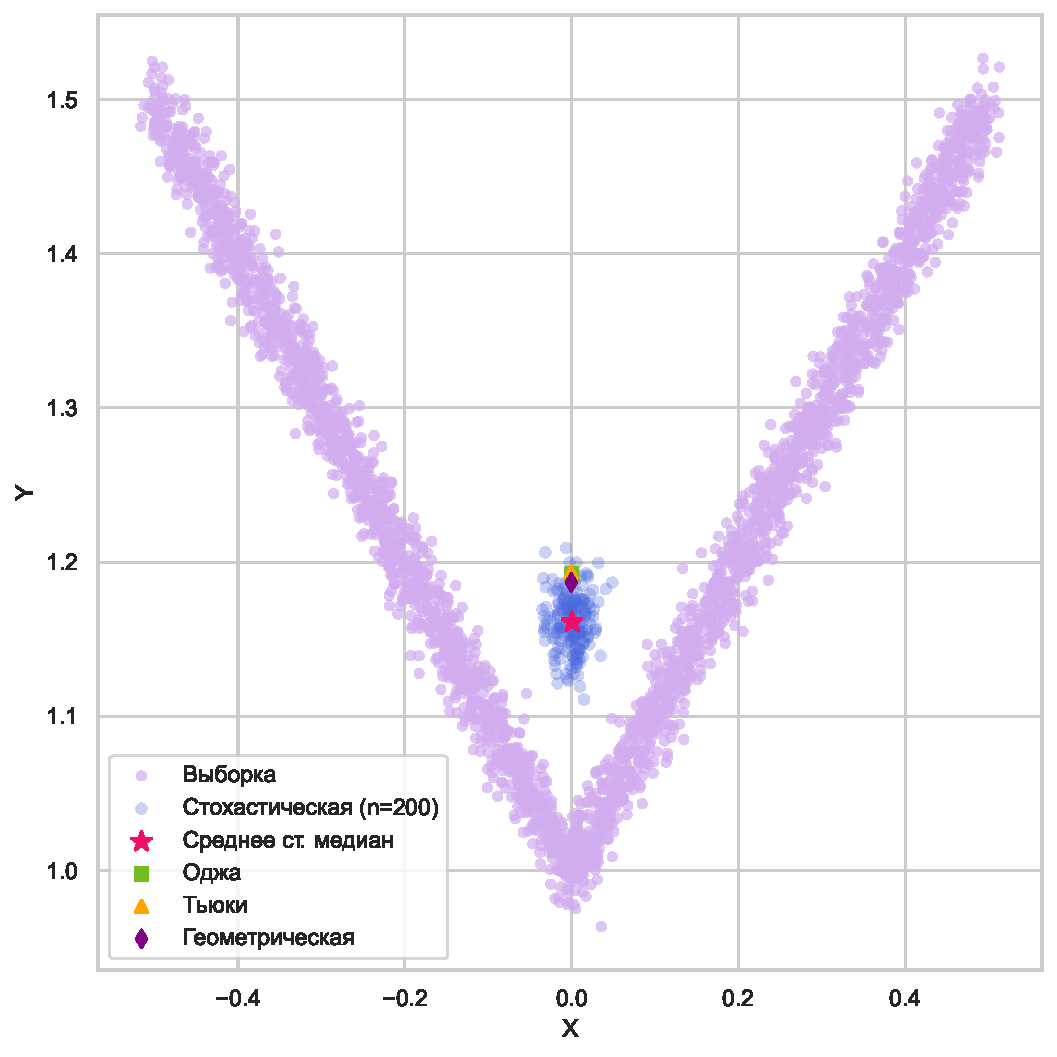
\includegraphics[width=\textwidth]{sample_V_ada.pdf}
%     \captionsetup{labelformat=empty}
%     \caption{(c) Ada}
%     \label{fig:V_rel_ada}
%   \end{subfigure}
%   \begin{subfigure}[b]{0.4\textwidth}
%     \centering
%     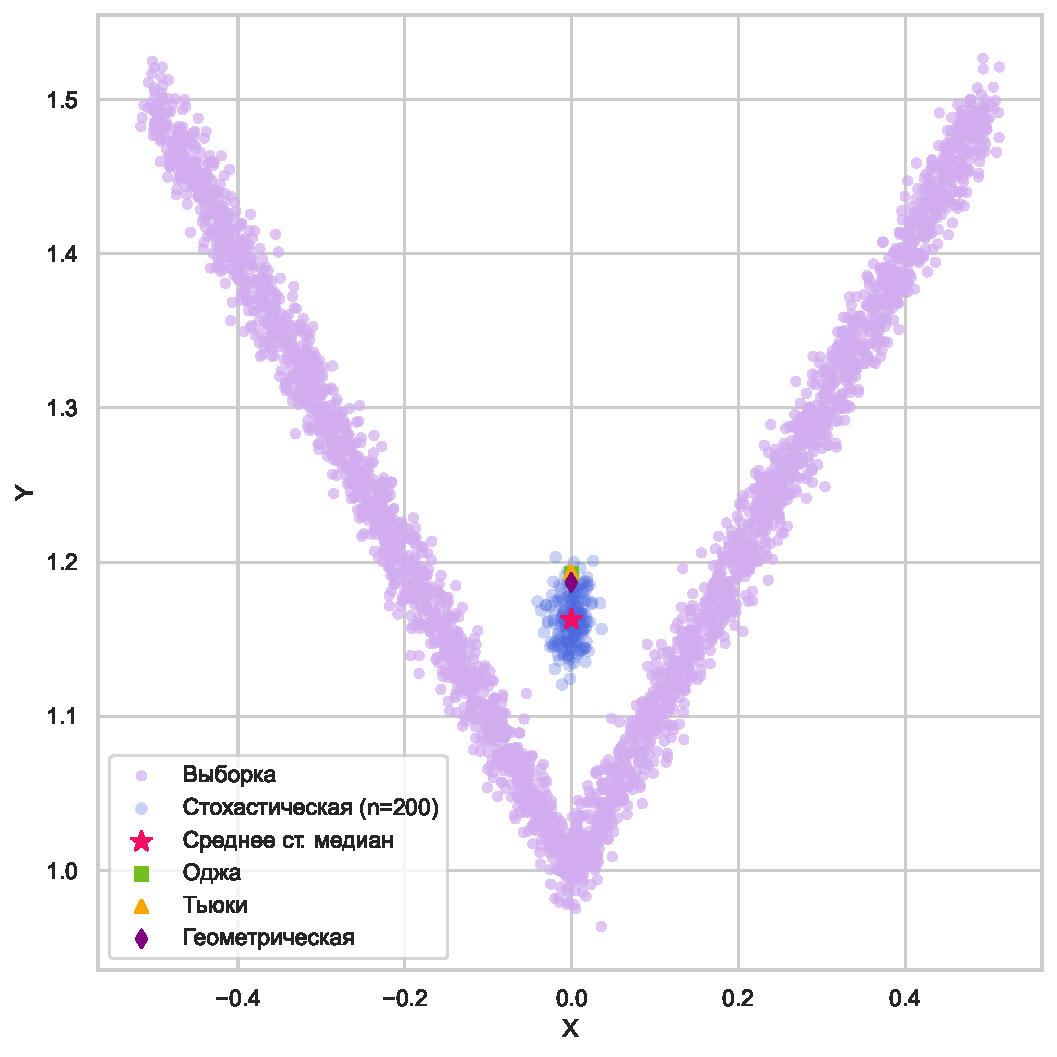
\includegraphics[width=\textwidth]{sample_V_ada_avg.pdf}
%     \captionsetup{labelformat=empty}
%      \caption{(f) Ada + Avg}
%      \label{fig:V_rel_ada_avg}
%   \end{subfigure}
%   \caption{Результат работы различных модификаций алгоритма на выборке, образующей букву V.}
%  \label{fig:V_comp}
% \end{figure}

% Рассмотрим также поведение алгоритма на выборке, образующей букву C. На этот раз сравним результаты, полученные при использовании относительного критерия останова, с результатами, полученными при использовании экспоненциального сглаживания и усреднения с параметрами, аналогичными использованным в предыдущем примере. 

% На рисунке~\ref{fig:C_comp} представлены результаты, демонстрирующие оценки многомерной медианы, полученные различными алгоритмами. Видно, что медианы Тьюки, Оджа, геометрическая, а также среднее значение, полученное на основе результатов работы стохастического алгоритма, сходятся к близким значениям. При этом сходимости для самой стохастической медианы в случае использования только относительного критерия не наблюдается (рис.~\ref{fig:C_rel}), так как полученные в результате работы алгоритма значения образуют облако с заметным разбросом точек внутри него. Если же рассматривать модификацию с экспоненциальным сглаживанием и усреднением (рис.~\ref{fig:C_exp_avg}), то облако становится существенно меньше, что позволяет сделать вывод о приблизительной сходимости алгоритма в данном случае.

% \begin{figure}[!hhh]
%   \centering
%   \begin{subfigure}[b]{0.45\textwidth}
%     \centering
%     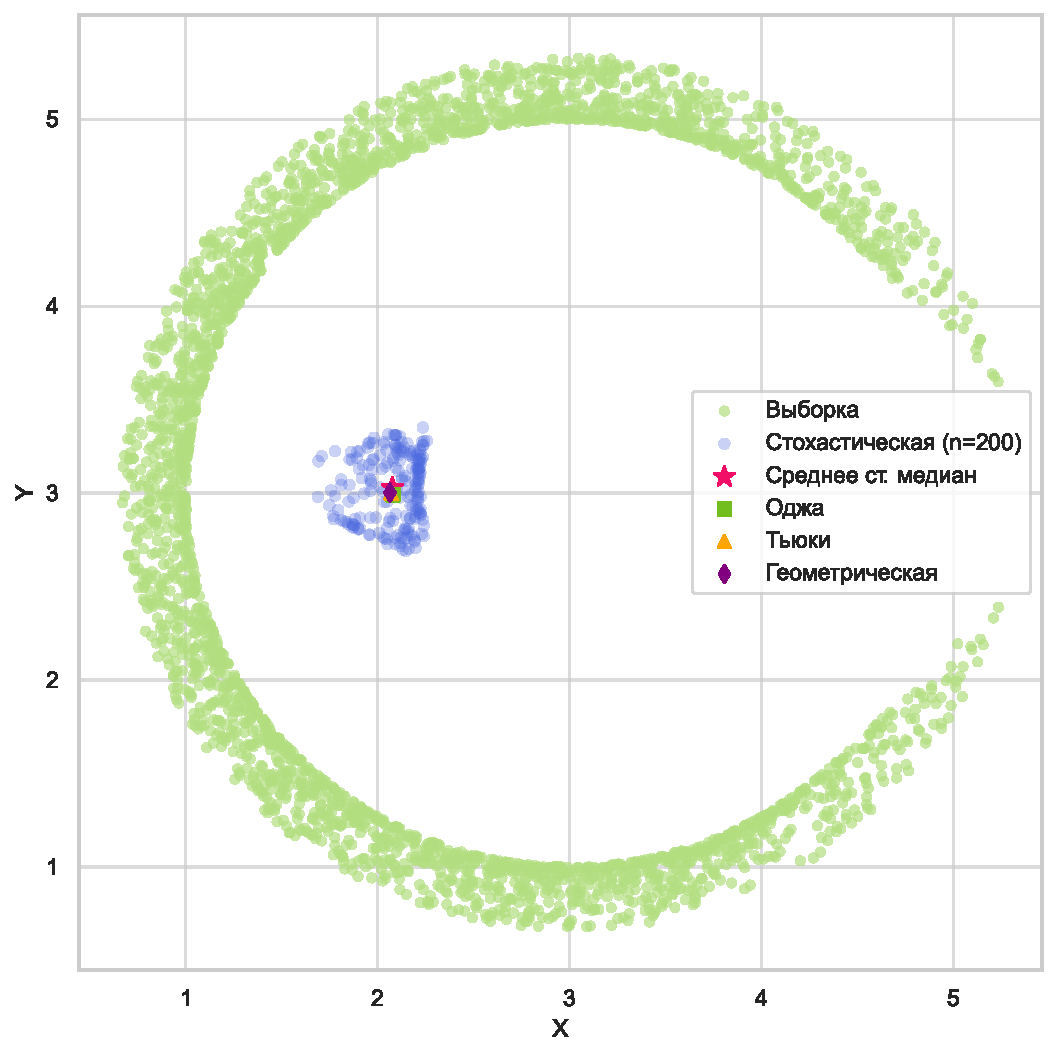
\includegraphics[width=\textwidth]{sample_C_base_new.pdf}
%     \captionsetup{labelformat=empty}
%      \caption{(a) Base}
%      \label{fig:C_rel}
%   \end{subfigure}
%    \hfill
%   \begin{subfigure}[b]{0.45\textwidth}
%     \centering
%     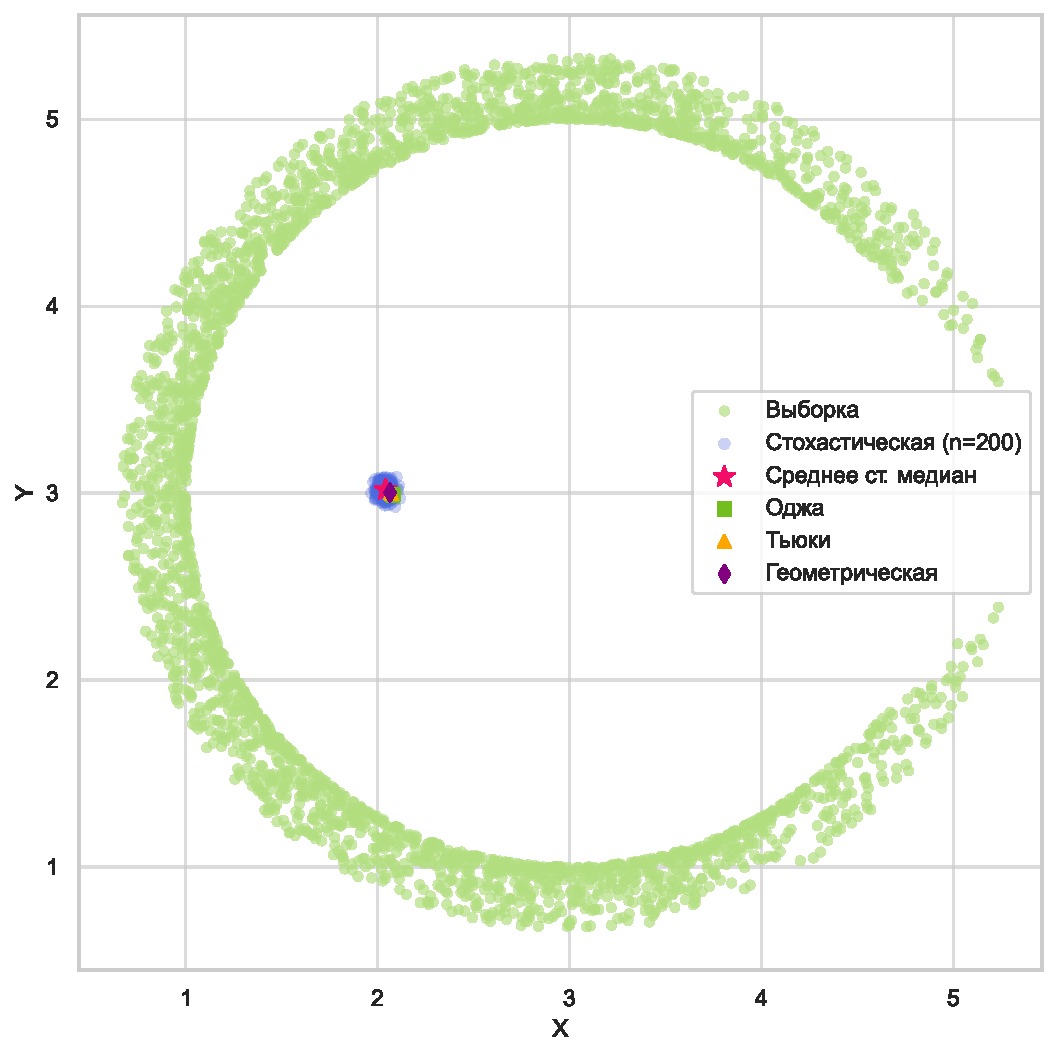
\includegraphics[width=\textwidth]{sample_C_exp_avg.pdf}
%     \captionsetup{labelformat=empty}
%     \caption{(b) Exp + Avg}
%     \label{fig:C_exp_avg}
%   \end{subfigure}

%   \caption{Результат работы различных модификаций алгоритма  на выборке, образующей букву C. }
%  \label{fig:C_comp}
% \end{figure}

% \newpage

% Рассмотрим двумерную выборку из $9$ точек, которые задают вложенные равносторонние треугольники на плоскости:
% \[
% (3; 2), \ (4; 3),\ (5; 4),\ (11; 2),\ (10; 3),\ (9; 4), \ (7; 2+ 4 \cdot \sqrt{3}),\ (7; 3+ 3 \cdot \sqrt{3}), \ (7; 4+ 2 \cdot \sqrt{3}).
% \]
% Центр тяжести в данном случае находится в точке $\left(7 \;\;   \frac{4\cdot\sqrt{3}}{6} + 4\right)^{\mathrm{T}}.$

% \vspace{1ex}

% % На рисунке \ref{fig:point_9} показаны результаты работы предложенного алгоритма и известных алгоритмов оценки параметра положения.   Алгоритмы, вычисляющие медиану Тьюки и геометрическую, дают наиболее близкие к ожидаемому результаты. Среднее также дает приемлемый результат. Медиана Оджа в данном случае далека от центра тяжести. 

% Предложенный стохастический алгоритм на данной выборке не сходится.  В этом можно убедиться, посмотрев на траекторию, которая является хаотичной (Рисунок \ref{fig:point_9_traj}). Алгоритм <<скачет>> от вершины к вершине внутреннего самого маленького треугольника и не может сойтись к центру тяжести.  

% \begin{figure}[!hhh]
%    \centering
%     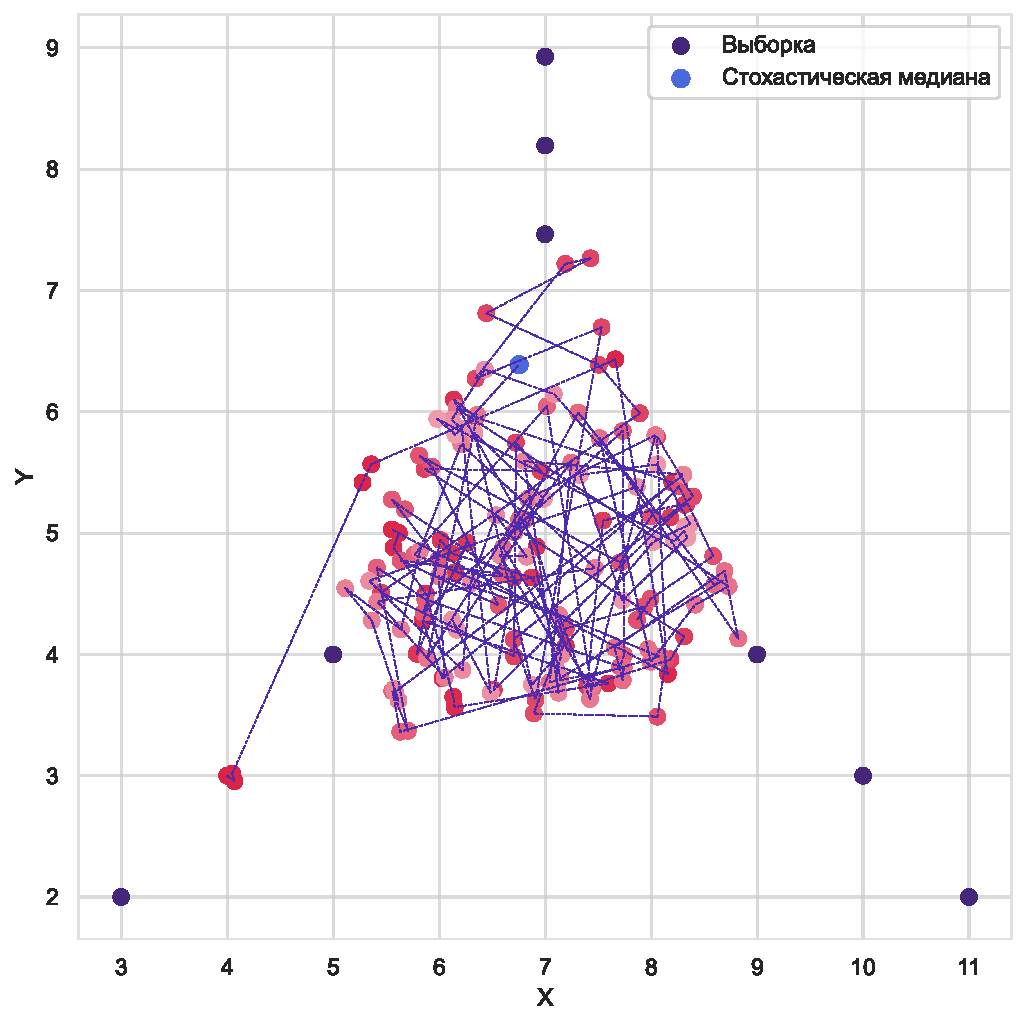
\includegraphics[width=0.6\textwidth]{sample_9point_4.pdf}
%   \caption{Траектория стохастического алгоритма для выборки из 9 точек.}
%   \label{fig:point_9_traj}
% \end{figure}

% % Посмотрим также на гистограмму ошибок на Рисунке \ref{fig:point_9_hist}, где ошибка определяется как разность полученного результата и мат. ожидания. На основе гистограммы можно сказать, что в большинстве случаев алгоритм скачет именно между тремя внутренними точками (так как в данном случае норма ошибки равна $\approx 1$--$1,5$).

% % \begin{figure}[!hhh]
% %    \centering
% %     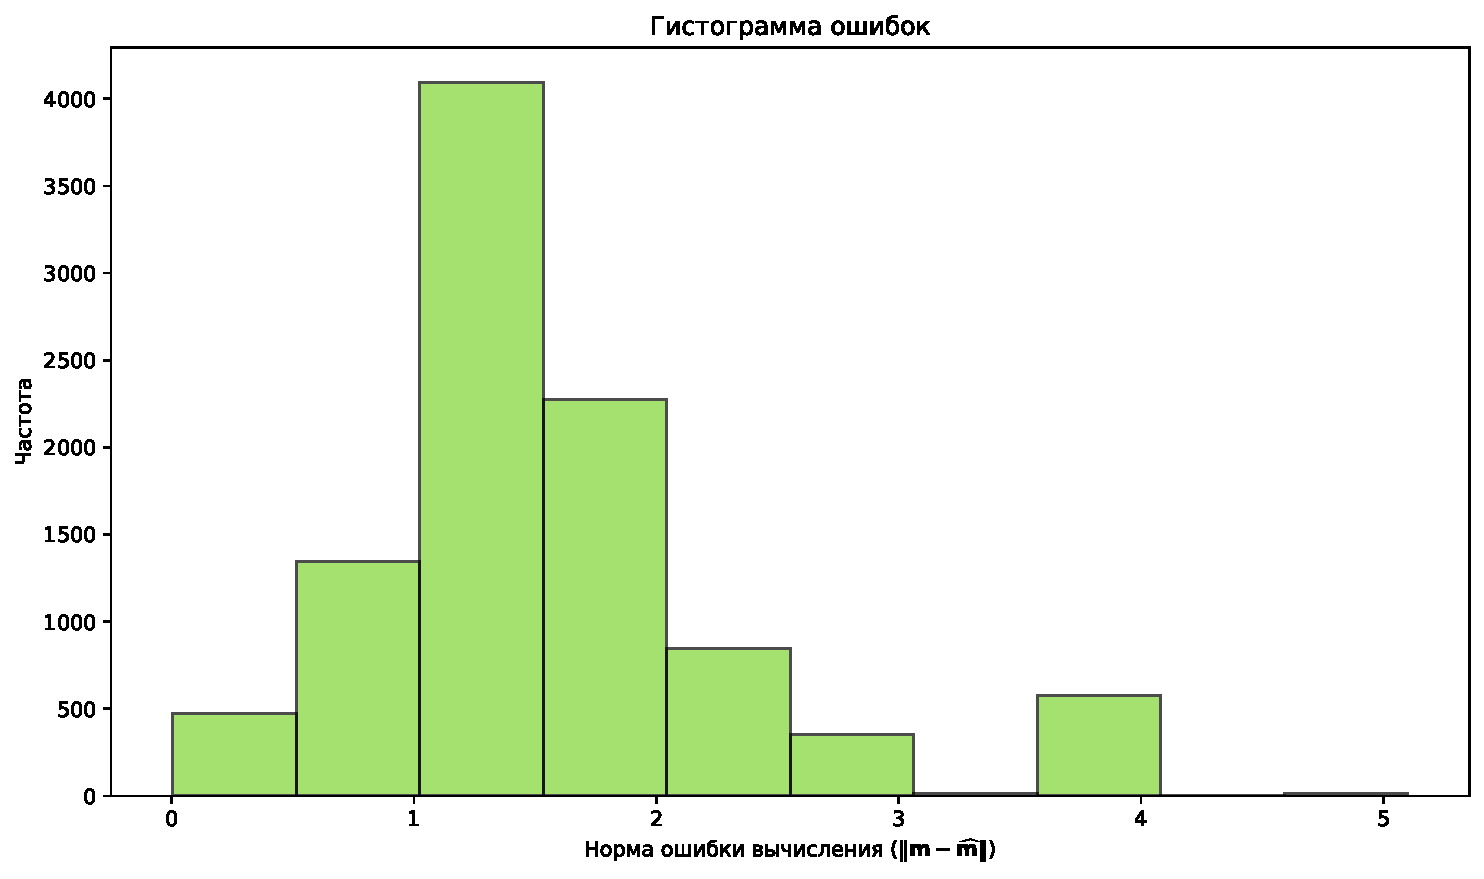
\includegraphics[width=14cm]{hist_9point.pdf}
% %   \caption{Алгоритм запускается 10000 раз на выборке из 9 точек. На основе полученных результатов строится гистограмма ошибок.}
% %   \label{fig:point_9_hist}
% % \end{figure}


% Анализ рисунка~\ref{fig:9point_comp} показывает, что на выборке, состоящей из вершин вложенных равносторонних треугольников, базовая версия алгоритма (рис.~\ref{fig:9point_rel}) не обеспечивает сходимость. Оценки <<скачут>> внутри треугольника, образованного самыми внутренними вершинами.

% Применение экспоненциального сглаживания значительно улучшает ситуацию (рис.~\ref{fig:9point_exp_avg}): выборка оценок образует компактное облако точек. При этом отклонение по каждой из осей от его центра (среднего значения полученных оценок) не превышает единицы, что свидетельствует о существенном повышении устойчивости алгоритма.

% \begin{figure}[!hhh]
%   \centering
%   \begin{subfigure}[b]{0.45\textwidth}
%     \centering
%     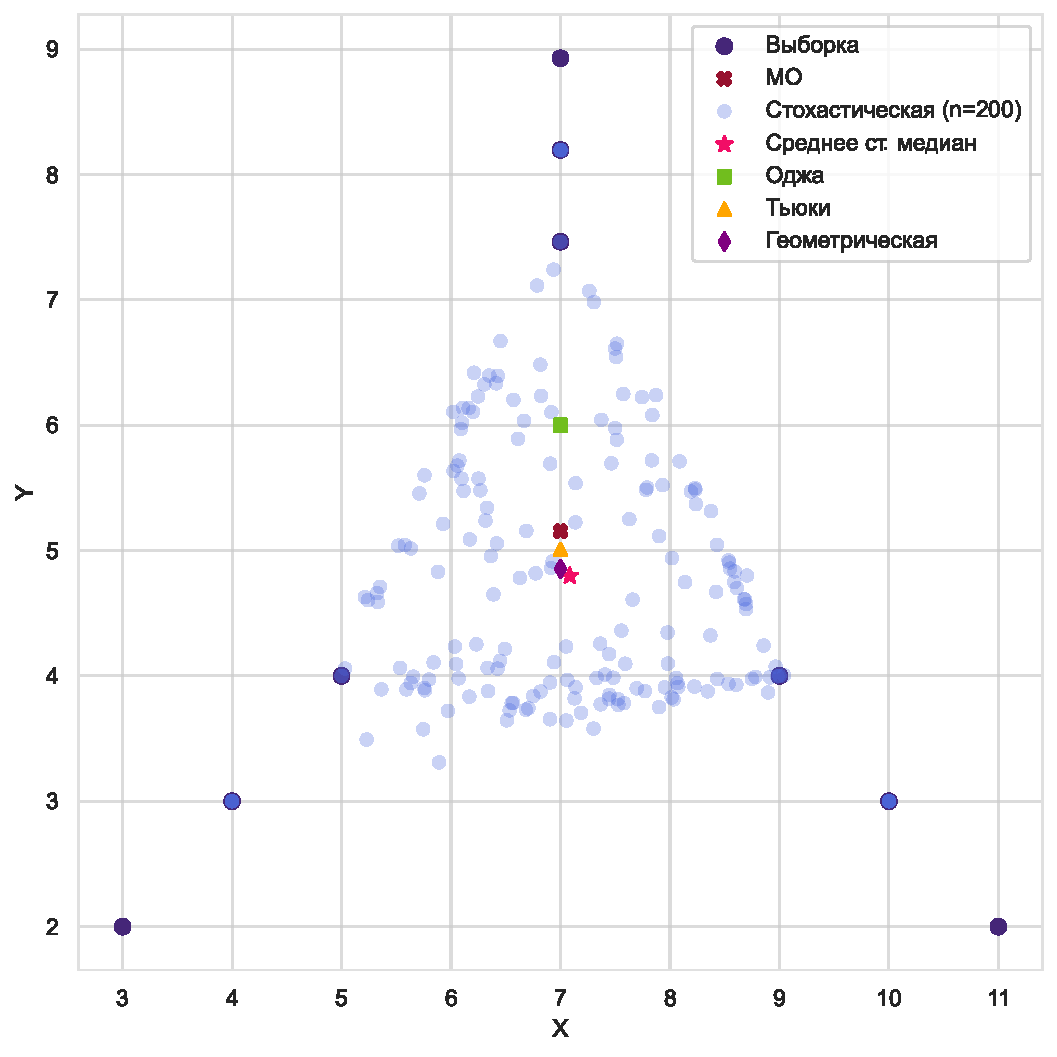
\includegraphics[width=\textwidth]{sample_9point_rel_crit_new.pdf}
%     \captionsetup{labelformat=empty}
%      \caption{(a) Base}
%      \label{fig:9point_rel}
%   \end{subfigure}
%    \hfill
%   \begin{subfigure}[b]{0.45\textwidth}
%     \centering
%     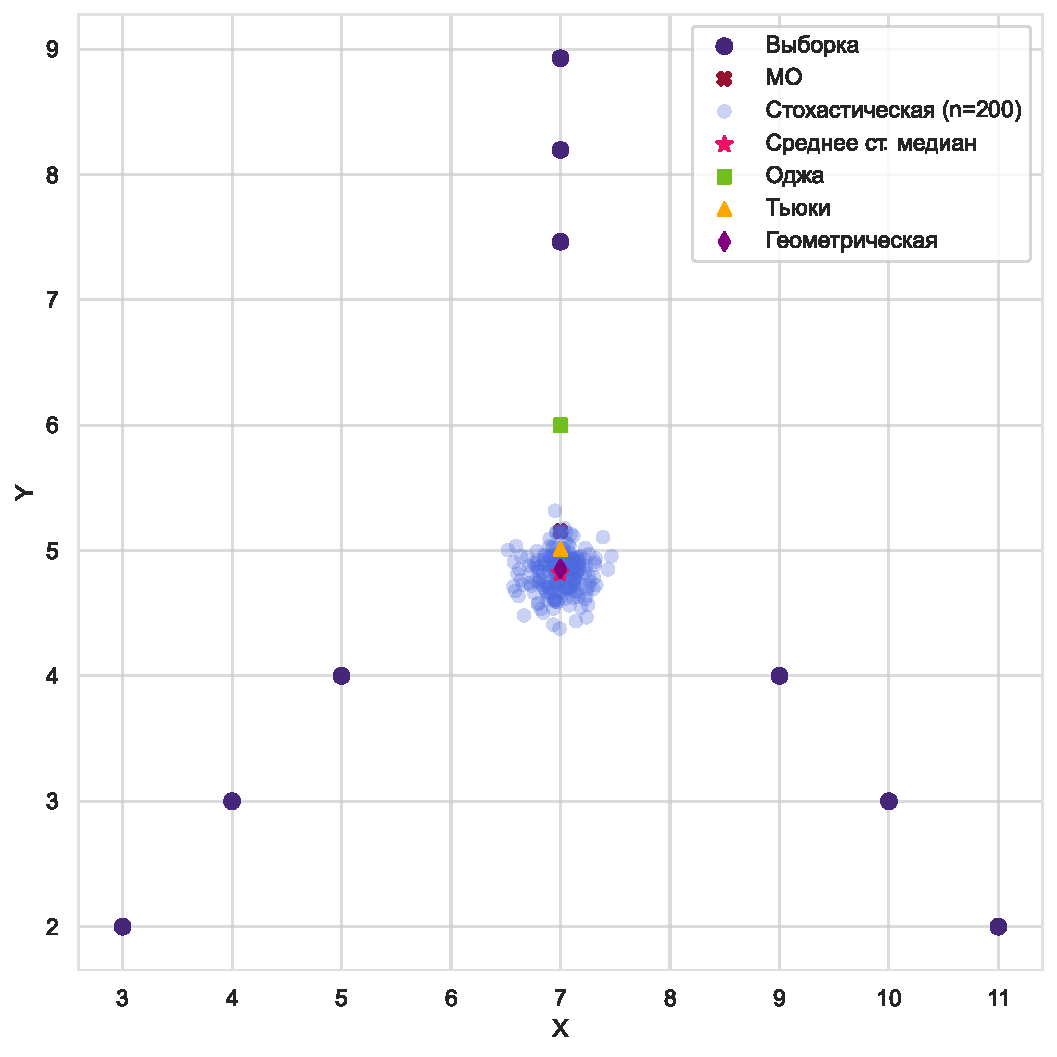
\includegraphics[width=\textwidth]{sample_9point_rel_crit_ada.pdf}
%     \captionsetup{labelformat=empty}
%     \caption{(b) Ada + Avg}
%     \label{fig:9point_exp_ada}
%   \end{subfigure}

%   \caption{Результат работы модификаций алгоритма на выборке из 9 точек --- вершин вложенных равносторонних треугольников.}
%  \label{fig:9point_comp}
% \end{figure}


\section{Рассмотрение случаев отсутствия сходимости алгоритма}

В предыдущих разделах было показано, что предложенные модификации позволяют уменьшить разброс оценок и повысить устойчивость алгоритма на выборках из стандартных распределений. Однако представляет интерес исследование случаев, в которых стохастический алгоритм испытывает трудности со сходимостью.

Далее рассматриваются несколько примеров выборок со сложной формой, для которых базовая версия алгоритма демонстрирует неустойчивое поведение. Основное внимание уделяется сравнению различных модификаций алгоритма и анализу того, насколько они позволяют уменьшить разброс оценок.

\subsection{Выборка, образующая букву V}

На Рисунке~\ref{fig:V_comp} представлены результаты работы различных модификаций алгоритма на выборке, образующей букву V. Для каждой модификации проводилось $200$ независимых запусков алгоритма.

Рассматриваются следующие варианты алгоритма:
\begin{itemize}
    \item базовая версия алгоритма с относительным критерием останова (Base);
    
    \item базовая версия с усреднением последних итераций (Base + Avg);
    
    \item алгоритм с экспоненциальным сглаживанием (Exp);
    
    \item алгоритм с экспоненциальным сглаживанием и усреднением (Exp + Avg);
    
    \item алгоритм с адаптивным выбором шага AdaGrad (AdaGrad);
    
    \item алгоритм AdaGrad с усреднением (AdaGrad + Avg).
\end{itemize}

Во всех случаях использовались многократное выполнение критерия останова и ограничение на минимальное число итераций, которое должен отработать алгоритм.

\begin{figure}[!htbp]
  \centering
  \begin{subfigure}[b]{0.32\textwidth}
    \centering
    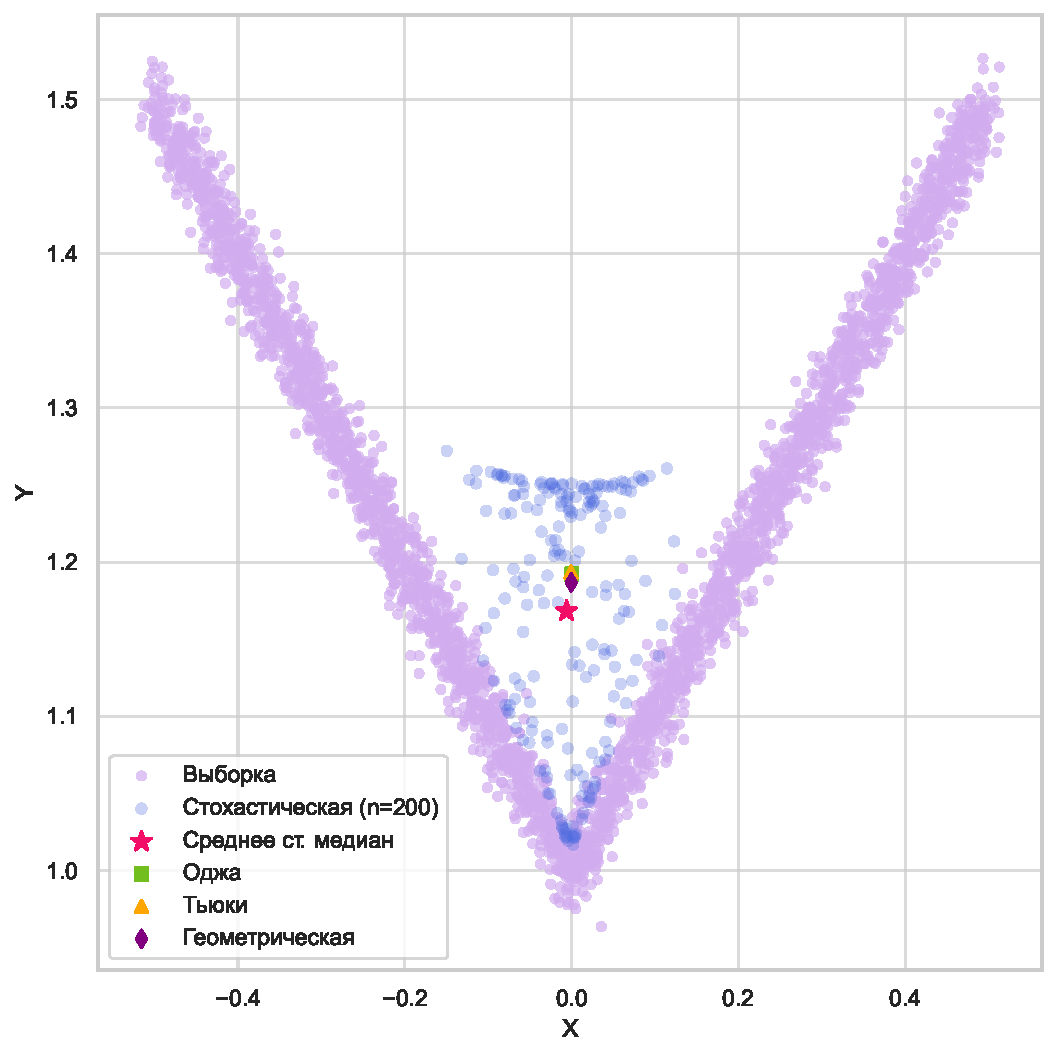
\includegraphics[width=\textwidth]{sample_V_base.pdf}
    \captionsetup{labelformat=empty}
     \caption{(а) Base}
     \label{fig:V_rel}
  \end{subfigure}
  \hfill
  \begin{subfigure}[b]{0.32\textwidth}
    \centering
    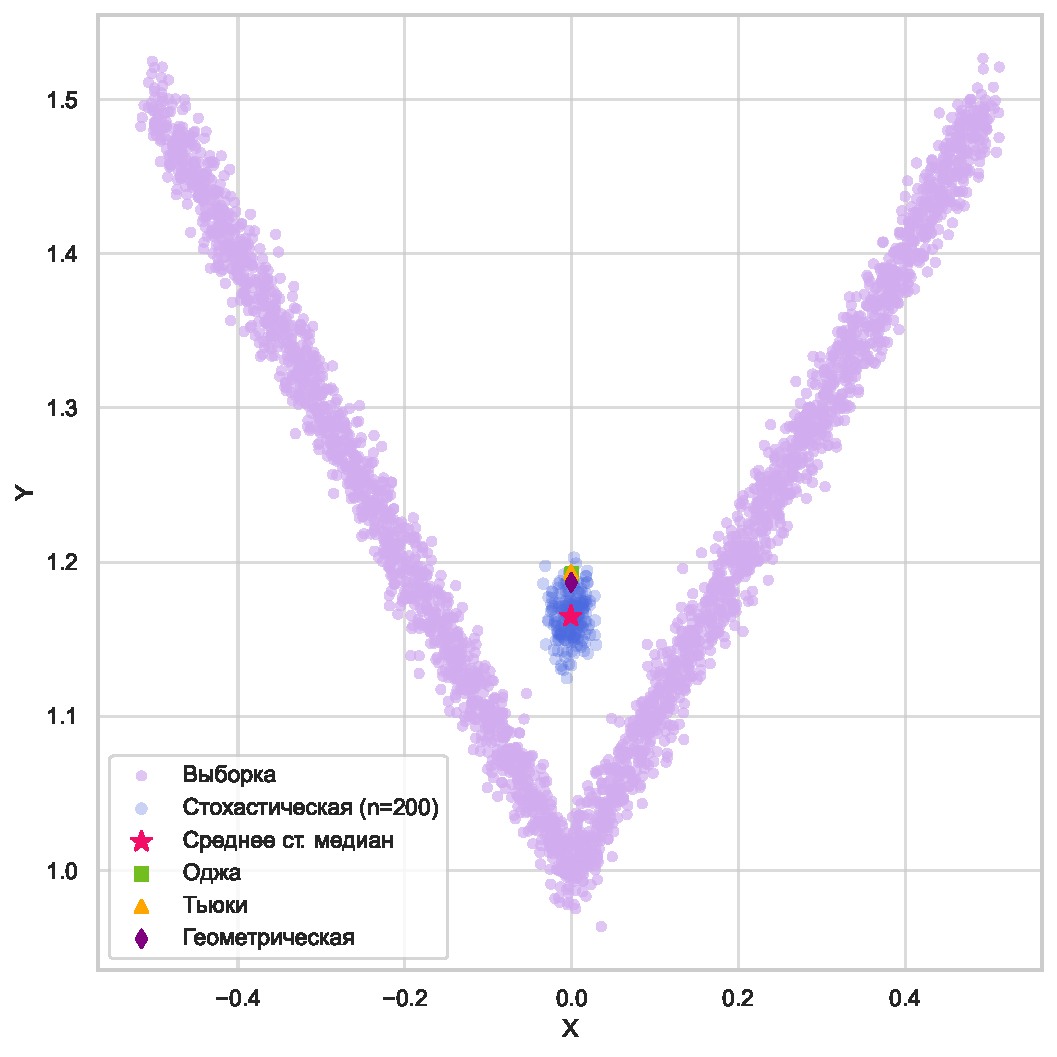
\includegraphics[width=\textwidth]{sample_V_exp.pdf}
    \captionsetup{labelformat=empty}
    \caption{(б) Exp}
   \label{fig:V_rel_exp}
  \end{subfigure}
  \hfill
  \begin{subfigure}[b]{0.32\textwidth}
    \centering
    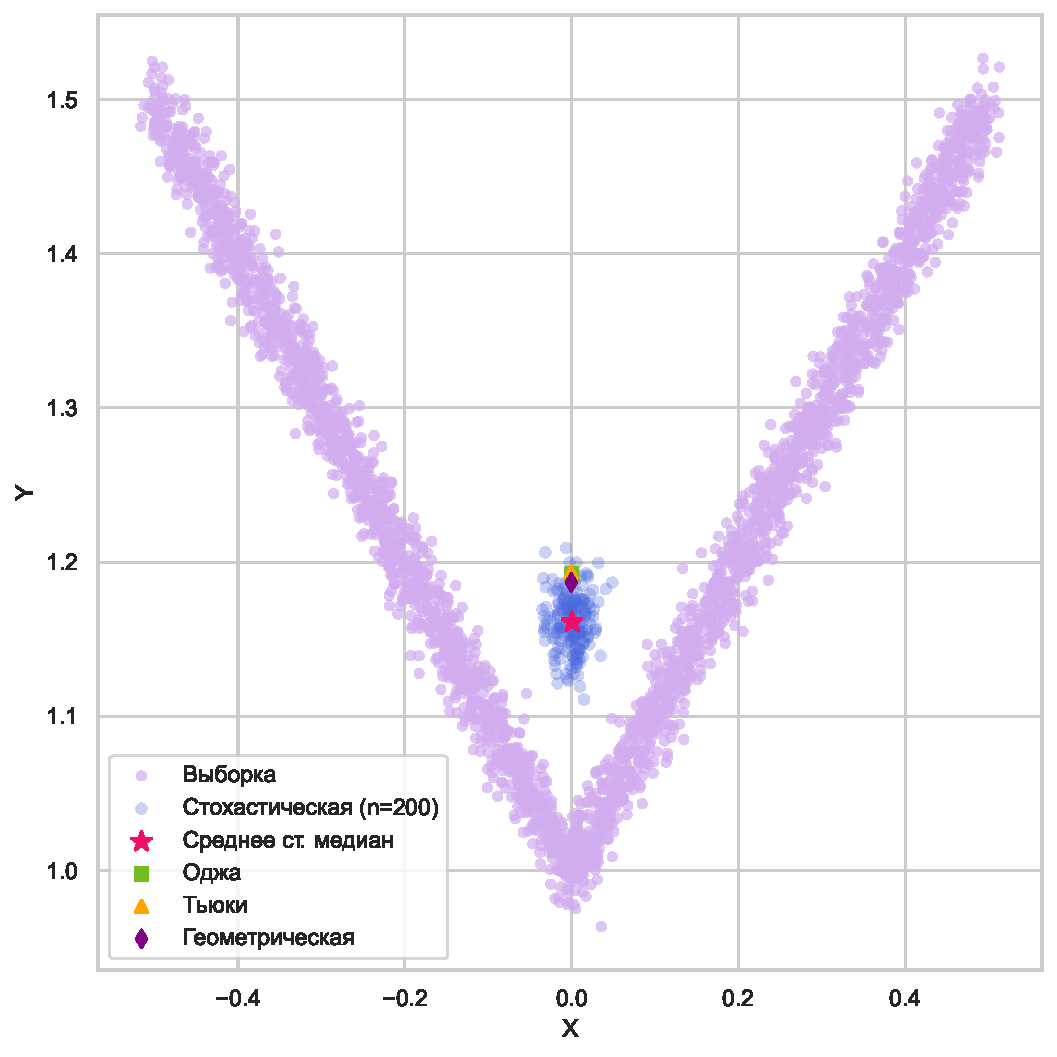
\includegraphics[width=\textwidth]{sample_V_ada.pdf}
    \captionsetup{labelformat=empty}
     \caption{(в) AdaGrad}
     \label{fig:V_rel_ada}
  \end{subfigure}

  \vspace{1ex}

  \begin{subfigure}[b]{0.32\textwidth}
    \centering
    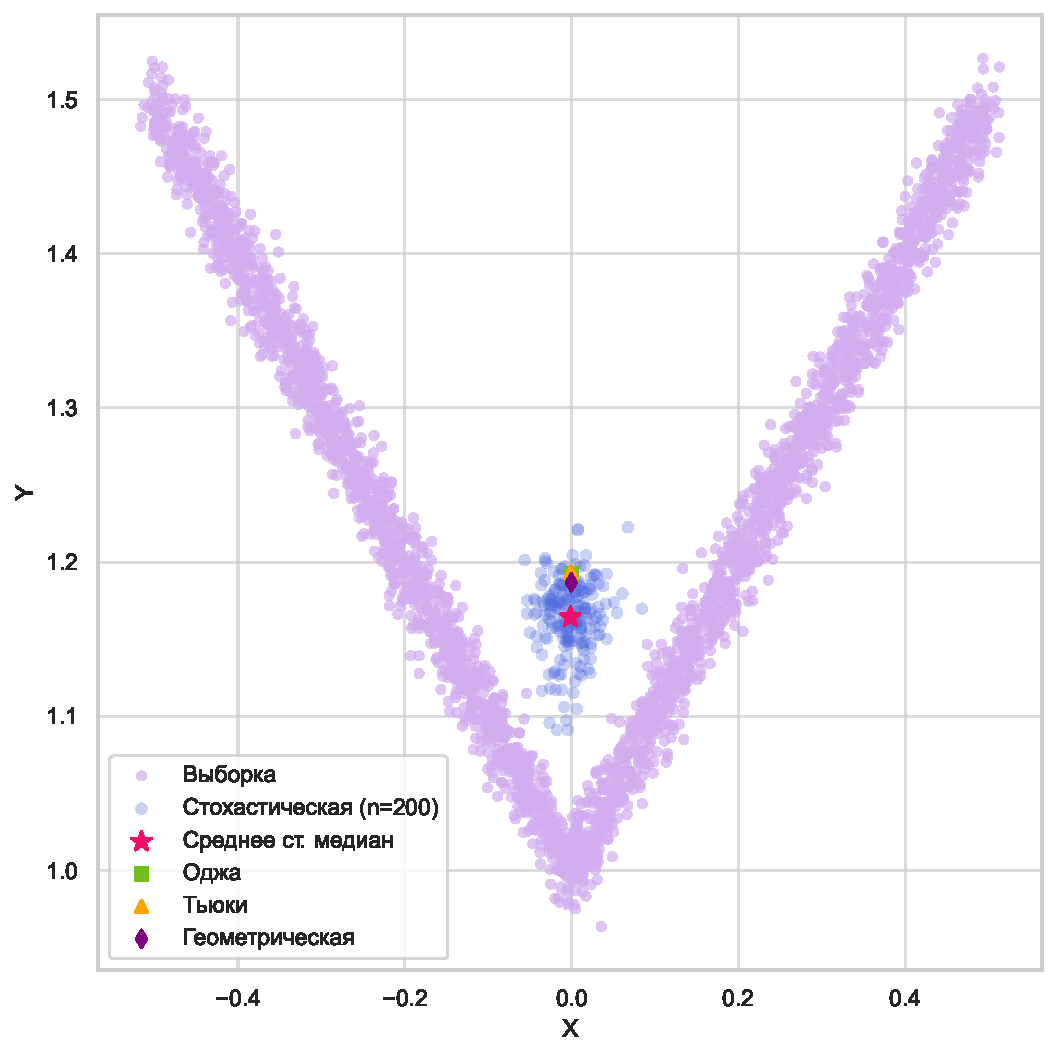
\includegraphics[width=\textwidth]{sample_V_base_avg.pdf}
    \captionsetup{labelformat=empty}
     \caption{(г) Base + Avg}
     \label{fig:V_rel_base_avg}
  \end{subfigure}
  \hfill
  \begin{subfigure}[b]{0.32\textwidth}
    \centering
    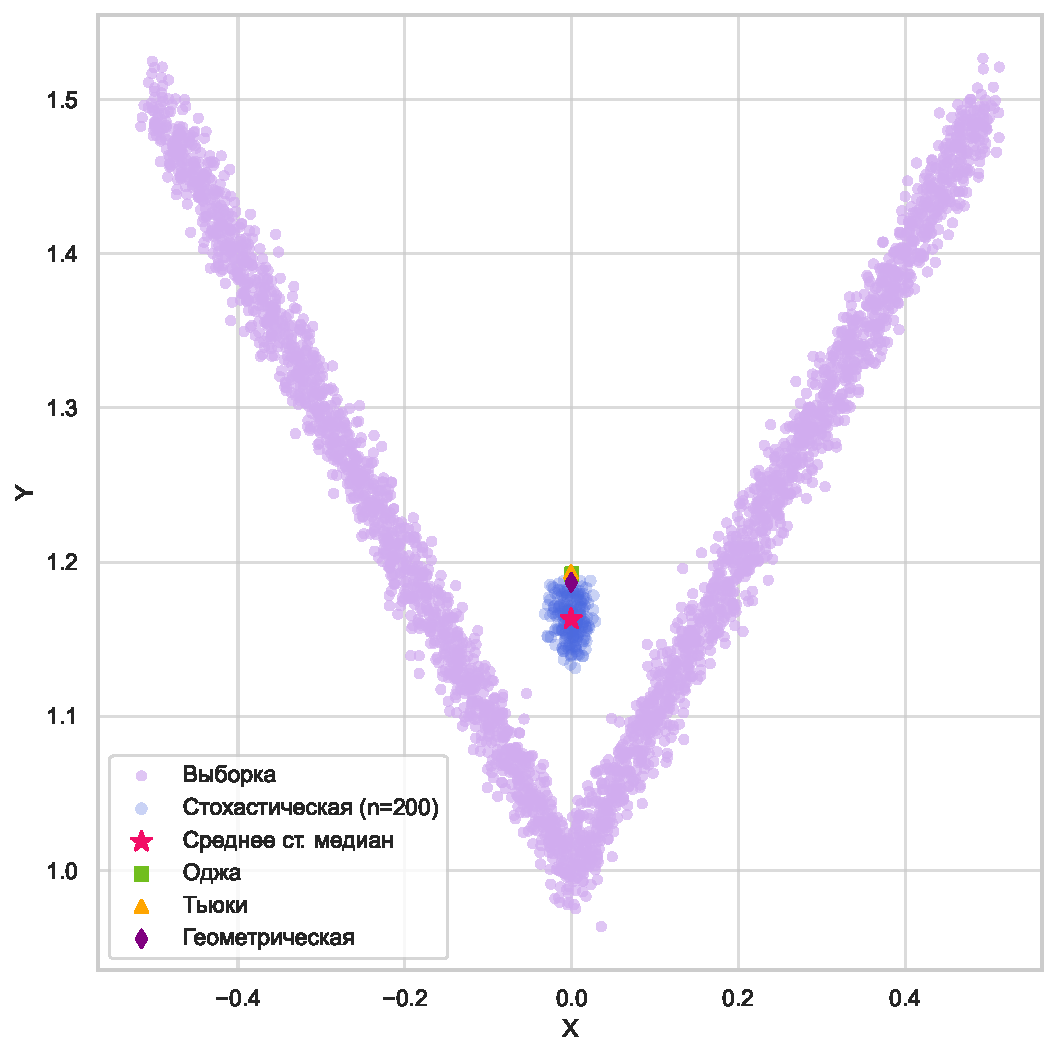
\includegraphics[width=\textwidth]{sample_V_exp_avg.pdf}
    \captionsetup{labelformat=empty}
    \caption{(д) Exp + Avg}
    \label{fig:V_rel_exp_avg}
  \end{subfigure}
  \hfill
  \begin{subfigure}[b]{0.32\textwidth}
    \centering
    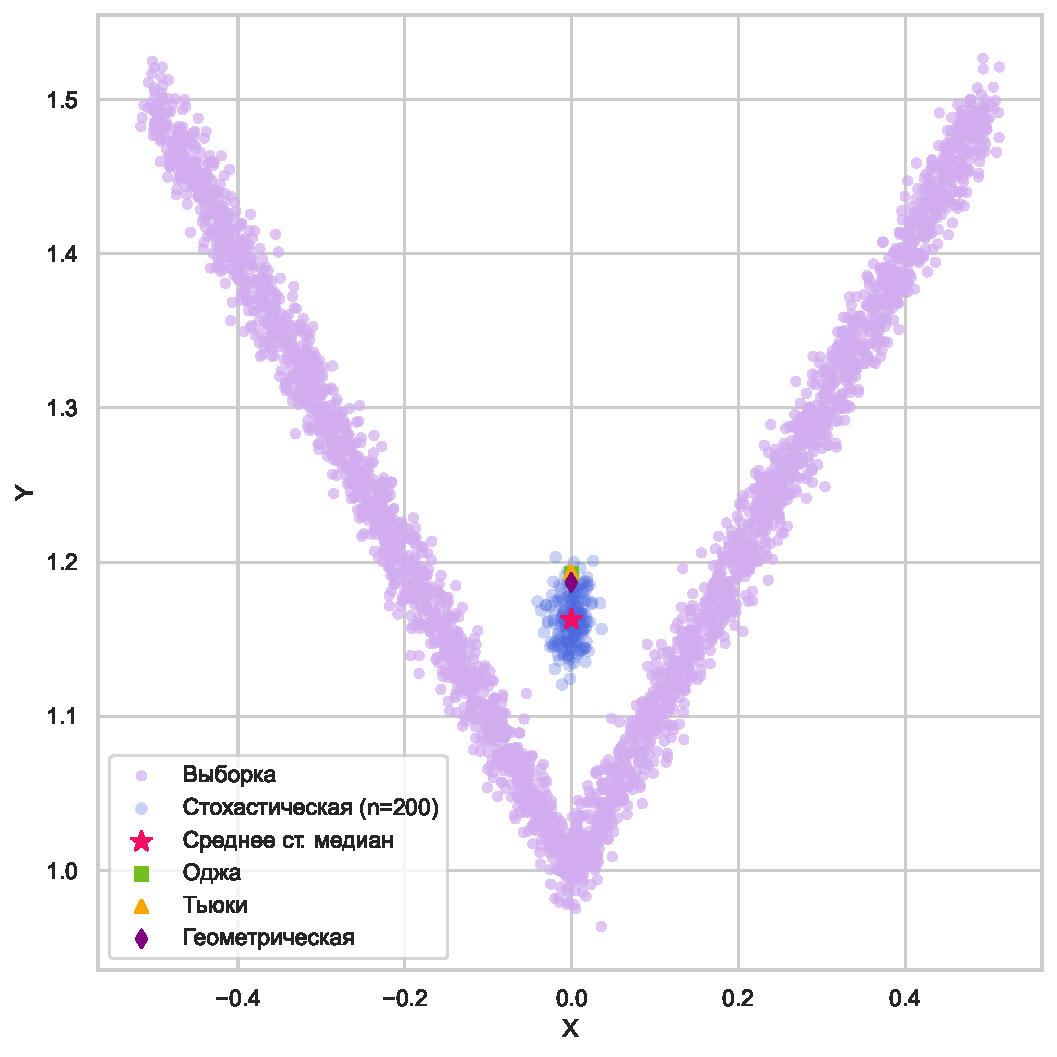
\includegraphics[width=\textwidth]{sample_V_ada_avg.pdf}
    \captionsetup{labelformat=empty}
     \caption{(е) AdaGrad + Avg}
     \label{fig:V_rel_ada_avg}
  \end{subfigure}

  \caption{Результаты работы различных модификаций алгоритма на выборке, образующей букву V.}
 \label{fig:V_comp}
\end{figure}

Из Рисунка~\ref{fig:V_comp} видно, что базовая версия алгоритма (Рис.~\ref{fig:V_rel}) демонстрирует значительный разброс оценок. Полученные значения образуют большое облако точек, вытянутое вдоль вертикального направления. При этом медианы Тьюки, Оджа и геометрическая медиана располагаются достаточно близко друг к другу.

Использование усреднения последних итераций (Рис.~\ref{fig:V_rel_base_avg}) позволяет уменьшить разброс оценок, однако облако точек остается достаточно широким.

Применение экспоненциального сглаживания (Рис.~\ref{fig:V_rel_exp}) приводит к существенному уменьшению разброса. Оценки становятся значительно более сконцентрированными около центра облака.

Наиболее устойчивые результаты наблюдаются при совместном использовании сглаживания и усреднения (Рис.~\ref{fig:V_rel_exp_avg}). В этом случае разброс оценок минимален, а облако точек становится существенно более компактным по сравнению с базовой версией алгоритма.

Модификация AdaGrad (Рис.~\ref{fig:V_rel_ada}) также уменьшает разброс оценок, однако итоговые результаты оказываются менее устойчивыми, чем при использовании экспоненциального сглаживания. Добавление усреднения (Рис.~\ref{fig:V_rel_ada_avg}) дополнительно улучшает ситуацию, однако распределение оценок все равно остается менее компактным по сравнению с методом Exp + Avg.

Таким образом, для выборки данного типа наилучшие результаты демонстрирует модификация с экспоненциальным сглаживанием и усреднением последних итераций.

\subsection{Выборка, образующая букву C}

Рассмотрим также поведение алгоритма на выборке, образующей букву C. В данном случае сравниваются базовая версия алгоритма и модификация с экспоненциальным сглаживанием и усреднением, показавшая наилучшие результаты.

\begin{figure}[!htbp]
  \centering
  \begin{subfigure}[b]{0.45\textwidth}
    \centering
    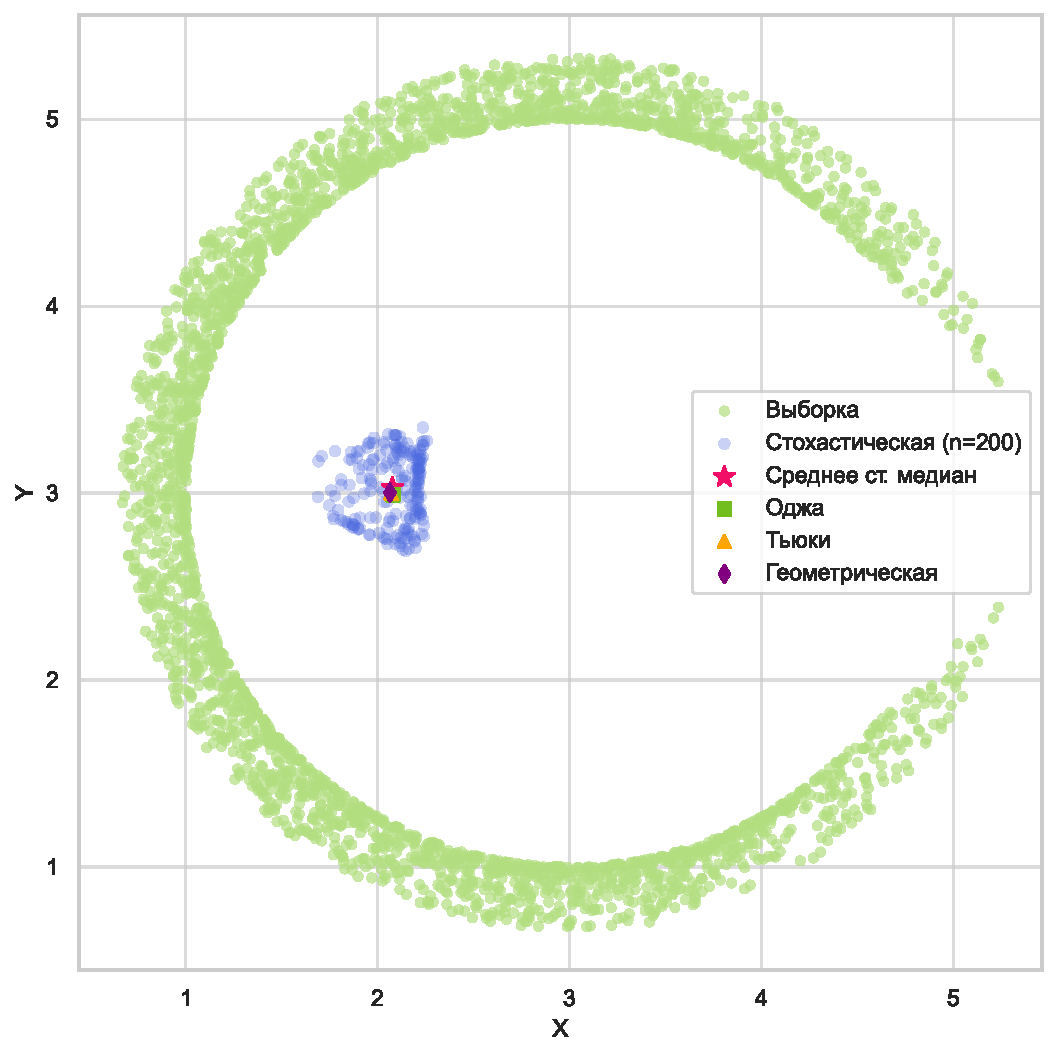
\includegraphics[width=\textwidth]{sample_C_base_new.pdf}
    \captionsetup{labelformat=empty}
     \caption{(а) Base}
     \label{fig:C_rel}
  \end{subfigure}
   \hfill
  \begin{subfigure}[b]{0.45\textwidth}
    \centering
    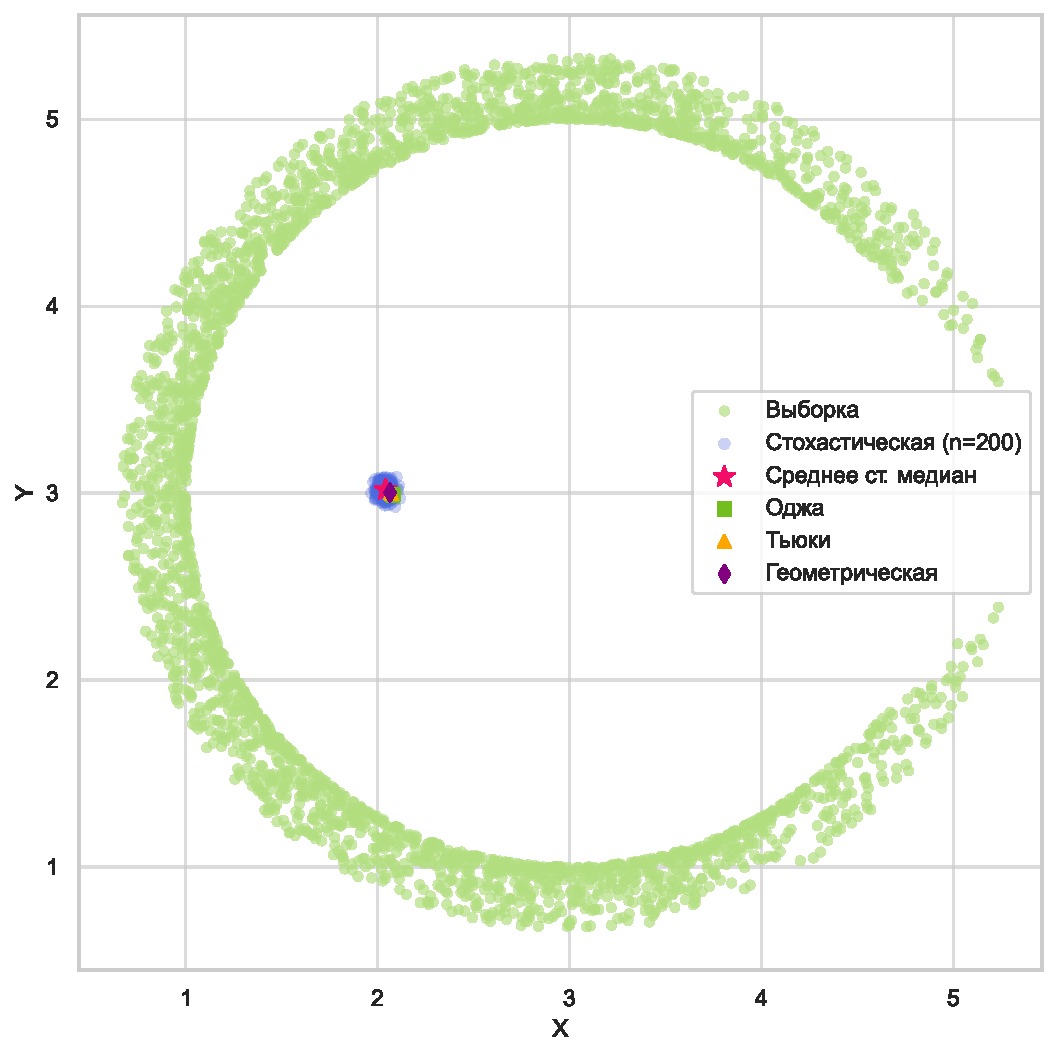
\includegraphics[width=\textwidth]{sample_C_exp_avg.pdf}
    \captionsetup{labelformat=empty}
    \caption{(б) Exp + Avg}
    \label{fig:C_exp_avg}
  \end{subfigure}

  \caption{Результаты работы различных модификаций алгоритма на выборке, образующей букву C.}
 \label{fig:C_comp}
\end{figure}

На Рисунке~\ref{fig:C_comp} видно, что базовая версия алгоритма (Рис.~\ref{fig:C_rel}) не обеспечивает устойчивой сходимости: полученные оценки образуют облако с заметным разбросом.

Использование экспоненциального сглаживания совместно с усреднением (Рис.~\ref{fig:C_exp_avg}) существенно уменьшает размеры облака и делает оценки значительно более стабильными. При этом результаты оказываются близкими к медианам Тьюки, Оджа и геометрической медиане.

Таким образом, даже в случае сложной невыпуклой геометрии модификация Exp + Avg позволяет существенно повысить устойчивость алгоритма.

\subsection{Выборка из вершин вложенных треугольников}

Рассмотрим двумерную выборку из $9$ точек, задающих вершины вложенных равносторонних треугольников:
\begin{align*}
(3; 2)^{\mathrm{T}}, \ (4; 3)^{\mathrm{T}},\ (5; 4)^{\mathrm{T}},\ (11; 2)^{\mathrm{T}},\ (10; 3)^{\mathrm{T}},\ (9; 4)^{\mathrm{T}}, \\ (7; 2+ 4 \cdot \sqrt{3})^{\mathrm{T}},\ (7; 3+ 3 \cdot \sqrt{3})^{\mathrm{T}}, \ (7; 4+ 2 \cdot \sqrt{3})^{\mathrm{T}}.    
\end{align*}

Центр тяжести в данном случае находится в точке $\left(7 ;   \frac{4\cdot\sqrt{3}}{6} + 4\right)^{\mathrm{T}}.$

\vspace{1ex}

На данной выборке базовая версия алгоритма не сходится, это можно увидеть по траектории последовательных приближений на Рисунке~\ref{fig:point_9_traj}.

\begin{figure}[!htbp]
   \centering
    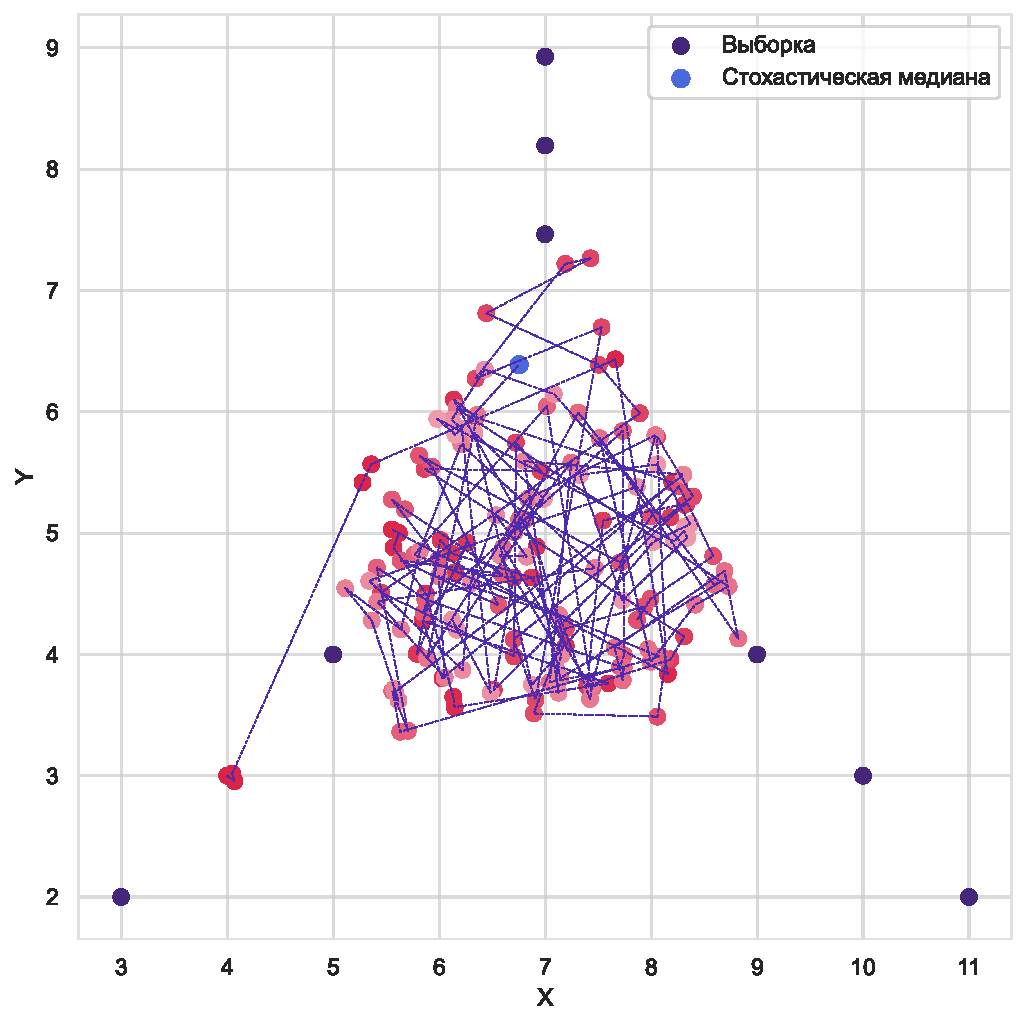
\includegraphics[width=0.5\textwidth]{sample_9point_4.pdf}
    \vspace{-2.75ex}
    
  \caption{Траектория базового алгоритма для выборки из 9 точек.}
  \label{fig:point_9_traj}
\end{figure}

На Рисунке~\ref{fig:point_9_traj} видно, что алгоритм хаотично перемещается между вершинами внутреннего треугольника и не стабилизируется около одной точки. В результате последовательность приближений не демонстрирует сходимости.

Далее сравним базовую версию алгоритма и модификацию AdaGrad с усреднением, которая показала наилучшие результаты для данной выборки.

\begin{figure}[!htbp]
  \centering
  \begin{subfigure}[b]{0.45\textwidth}
    \centering
    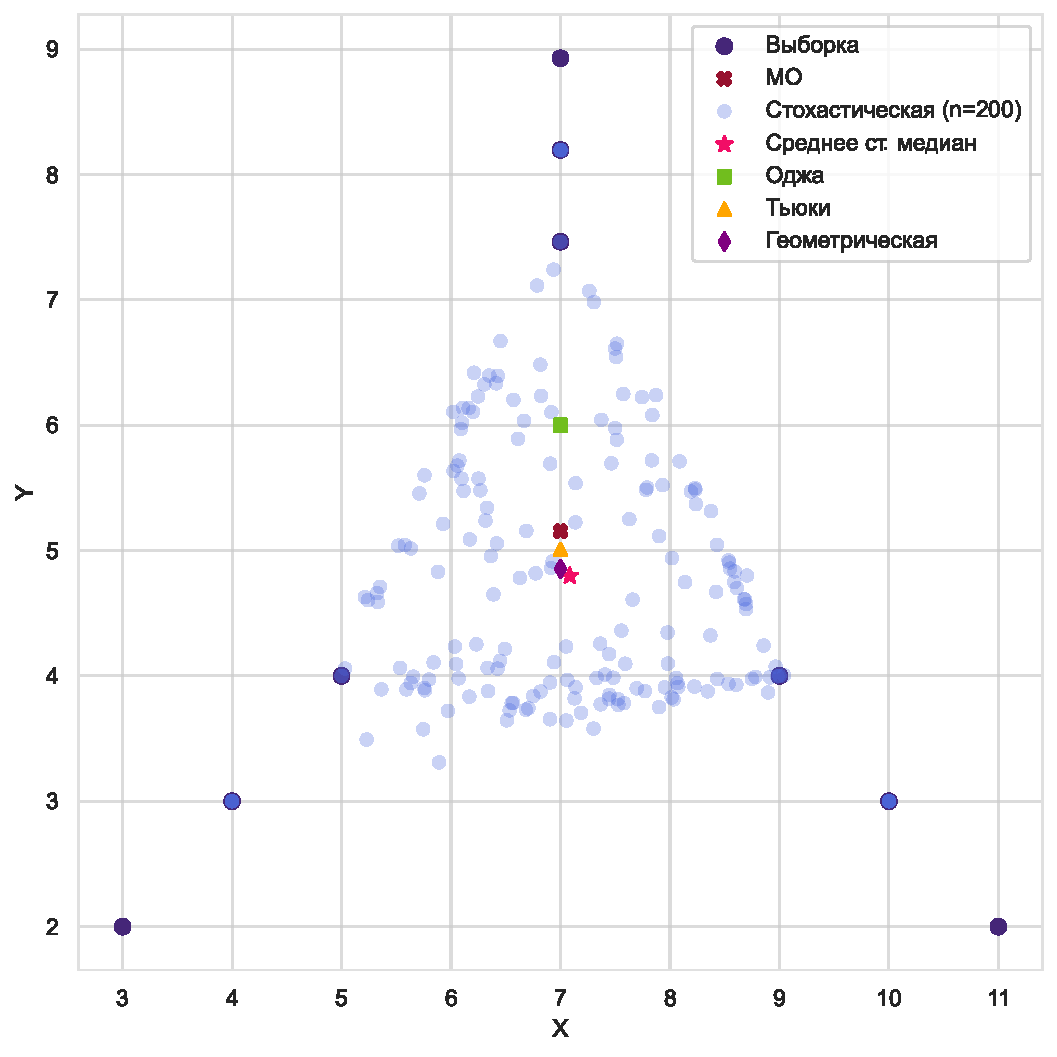
\includegraphics[width=\textwidth]{sample_9point_rel_crit_new.pdf}
    \captionsetup{labelformat=empty}
     \caption{(а) Base}
     \label{fig:9point_rel}
  \end{subfigure}
   \hfill
  \begin{subfigure}[b]{0.45\textwidth}
    \centering
    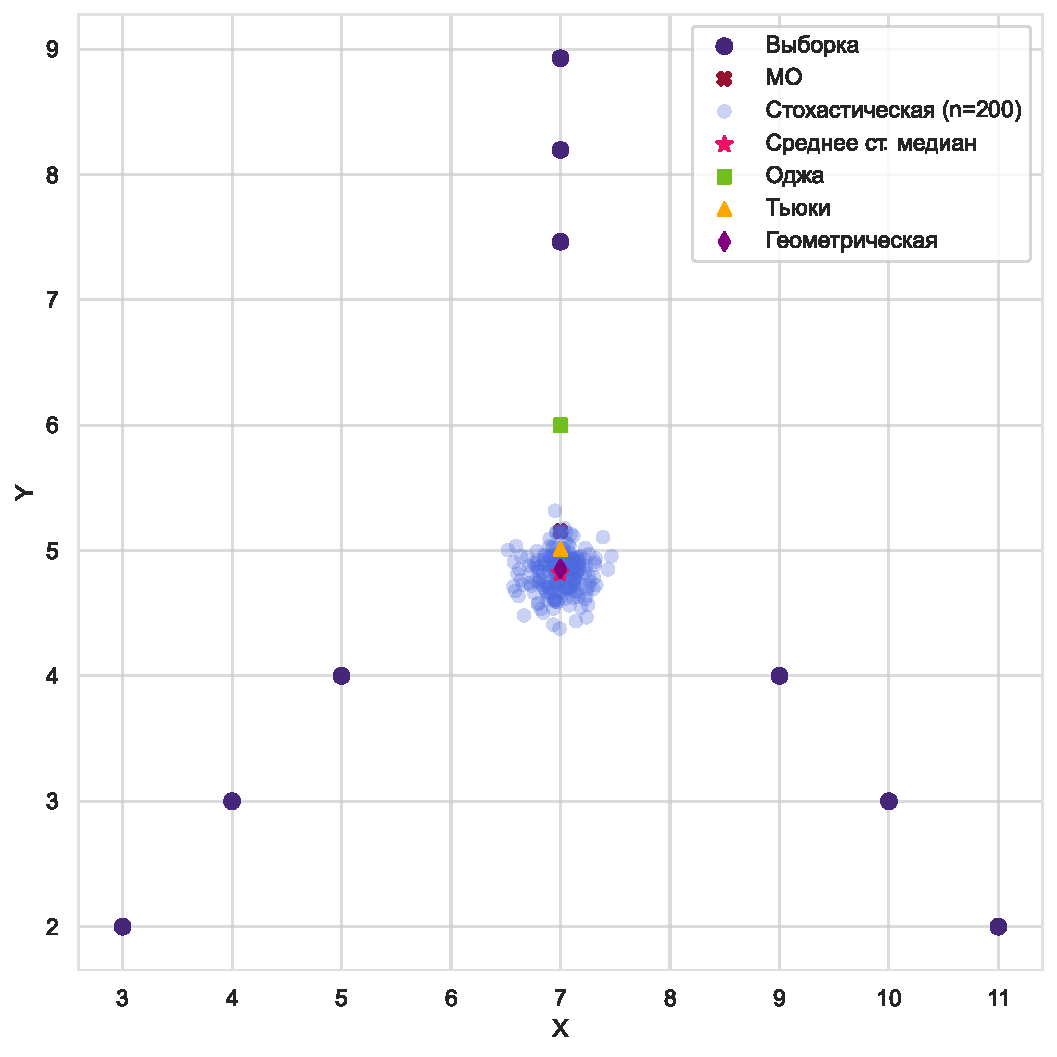
\includegraphics[width=\textwidth]{sample_9point_rel_crit_ada.pdf}
    \captionsetup{labelformat=empty}
    \caption{(б) AdaGrad + Avg}
    \label{fig:9point_exp_ada}
  \end{subfigure}

  \caption{Результаты работы модификаций алгоритма на выборке из вершин вложенных равносторонних треугольников.}
 \label{fig:9point_comp}
\end{figure}

На Рисунке~\ref{fig:9point_comp} видно, что базовая версия алгоритма (Рис.~\ref{fig:9point_rel}) дает большой разброс оценок внутри внутреннего треугольника.

Использование AdaGrad совместно с усреднением (Рис.~\ref{fig:9point_exp_ada}) позволяет существенно уменьшить разброс оценок и получить компактное облако точек около центра распределения.

Таким образом, рассмотренные примеры показывают, что базовая версия стохастического алгоритма может испытывать трудности со сходимостью на выборках со сложной формой. Однако использование модификаций траектории, особенно экспоненциального сглаживания и адаптивного выбора шага совместно с усреднением, позволяет значительно повысить устойчивость алгоритма и уменьшить разброс оценок.
\chapter{Оценка матрицы разброса}

В предыдущих главах рассматривались робастные методы оценивания многомерного параметра положения. Однако во многих задачах многомерного анализа требуется также робастная оценка матрицы разброса.

\section{Метод оценивания вдоль случайных направлений}

Для робастной оценки матрицы разброса $\mathbf{S} \in \mathbb{R}^{d \times d}$ воспользуемся идеей, применявшейся ранее в методах, основанных на алгоритмах концентрации (см. раздел~\ref{sec:concentration}). Модифицируем Алгоритм~\ref{alg:median} таким образом, чтобы на каждой итерации вместе с оценкой медианы вычислялось также медианное абсолютное отклонение ($\mathrm{MAD}$) вдоль выбранного направления.

В отличие от методов концентрации, здесь не используется процедура отбрасывания части выборки. Вместо этого информация о разбросе данных извлекается из проекций выборки на случайные направления.

\textbf{Идея метода}

Известно, что проекция многомерной случайной величины с ковариационной матрицей $\boldsymbol{\Sigma}$ на направление $\mathbf{u}$ имеет дисперсию $\sigma^2 = \sigma^2_{\mathbf{u}} = \mathbf{u}^{\mathrm{T}} \boldsymbol{\Sigma} \mathbf{u}$.

В общем случае заменим матрицу $\boldsymbol{\Sigma}$  на $\mathbf{S}$, а $\sigma^2_{\mathbf{u}}$ на
\begin{equation}\label{eq:mad}
    \widehat{\text{MAD}}^2_{\mathbf{u}} = \left(\frac{1}{\Phi^{-1}(3/4)} \text{MAD}_{\mathbf{u}}\right)^2,
\end{equation}
где $\Phi$ ---  функция распределения стандартной нормальной величины. Коэффициент $\Phi^{-1}(3/4)$ возникает из известного соотношения между MAD и среднеквадратическим отклонением для нормального распределения.

Таким образом, вводится нормировка, чтобы в случае нормального распределения матрица разброса сходилась к ковариационной матрице с ростом размера выборки. 

Пусть на $i$-й итерации Алгоритма~\ref{alg:median} выбрано случайное направление $\mathbf{u}_i$. Для него вычислим величину $\widehat{\mathrm{MAD}}_{\mathbf{u}_i}^2$. По аналогии с нормальной моделью будем считать, что выполняется приближенное соотношение
\begin{equation}\label{eq_mad}
    \widehat{\mathrm{MAD}}_{\mathbf{u}_i}^2
    \approx
    \mathbf{u}^{\mathrm{T}}_i\mathbf{S}\mathbf{u}_i.
\end{equation}

Тогда задача оценки матрицы $\mathbf{S}$ сводится к оценке её элементов, используя соотношение \eqref{eq_mad}.

Поскольку матрица $\mathbf{S}$ симметрична, достаточно оценивать только элементы верхнего треугольника $s_{11}$, \ldots, $s_{ij}$, \ldots, $s_{dd}$, $i \leqslant j$. 
Общее число неизвестных параметров равно $r = \frac{d(d+1)}{2}$.

Пусть $\mathbf{u}_i = (u_1^i, \ldots, u_d^i)^\rmT$. Тогда выражение $\mathbf{u}_i^{\mathrm{T}}\mathbf{S}\mathbf{u}_i$
является линейной комбинацией элементов матрицы $\mathbf{S}$:
% Тогда $\mathbf{u}_i^\rmT \mathbf{S} \mathbf{u}_i$ для $i = 1, \ldots, k$ (где $k$ --- общее число итераций Алгоритма~\ref{alg:median}) являются линейными
% комбинациями элементов $s_{i, j}$. Пусть $\mathbf{u}_i = (u_1^i, \ldots, u_d^i)^\rmT$, тогда верно следующее:
\begin{equation}\label{eq:linearform}
    \mathbf{u}_i^\rmT \mathbf{S} \mathbf{u}_i = \sum_{j = 1}^d (u_j^i)^2 s_{jj} + \sum_{1 \leqslant j < p \leqslant d} 2 u_j^i u_p^i s_{jp},
\end{equation}
где $i = 1, \ldots, K$, а $K$ --- общее число итераций Алгоритма~\ref{alg:median}.

Следовательно, используя несколько случайных направлений, можно получить систему линейных уравнений относительно неизвестных коэффициентов~$s_{ij}$.

Для каждого направления $\mathbf{u}_i$ сформируем строку матрицы регрессоров $\hat{\mathbf{X}}\in \mathbb{R}^{K \times r}$ из коэффициентов $(u_j^i)^2$ и $u_j^i u_p^i$ перед элементами $s_{ij}$ в выражении~\eqref{eq:linearform}. Соответствующие значения $\widehat{\mathrm{MAD}}_{\mathbf{u}_i}^2$ образуют вектор $\mathbf{z} \in \mathbb{R}^K$.

% Следовательно, если для каждого $i$ взять коэффициенты $(u_j^i)^2$ и $u_j^i u_k^i$ перед элементами $s_{i, j}$ из \eqref{eq:linearform}, всего $r$ штук, и составить из них матрицу регрессоров $\mathbf{X} \in \mathbb{R}^{k \times r}$, а элементы из $\widehat{\text{MAD}}^2_{\mathbf{u}_i}$ положить в вектор $\mathbf{y} \in \mathbb{R}^k$,
% то используя выражение \eqref{eq_mad} для $i = 1, \ldots, k$  можем оценить коэффициенты $s_{i, j}$, $1 \le i \le j \le d$ (назовём
% эти оценки $\hat{\mathbf{s}} = (\hat s_{i, j})$, используя обычный линейный МНК для матрицы-регрессора $\mathbf{X}$ и зависимого вектора $\mathbf{y}$: $\hat{\mathbf{s}} = \mathbf{X}^- \mathbf{y},$ где $\mathbf{X}^-$ --- псевдообратная Мура-Пенроуза к $\mathbf{X}$.


Тогда задача оценки матрицы разброса сводится к линейной регрессии:
\begin{equation*}
\widehat{\mathbf{s}} = \hat{\mathbf{X}}^{-}\mathbf{z},
\end{equation*}
где $\hat{\mathbf{X}}^{-}$ --- псевдообратная матрица Мура--Пенроуза, а $\widehat{\mathbf{s}}=(\widehat{s}_{ij})$ --- оценки элементов матрицы разброса.

Таким образом, оценивание матрицы разброса сводится к восстановлению коэффициентов линейной системы, построенной по случайным направлениям и робастным оценкам масштаба вдоль этих направлений. Полученный метод представлен в виде Алгоритма~\ref{alg:dispercematrix_naive}.

Заметим, что минимально требующееся количество итераций $K$ для Алгоритма~\ref{alg:median} равно $r$, иначе выборка направлений будет недостаточной по размеру для построения оценки $\widehat{\mathbf{S}}$.

Кроме того, алгоритм эквивариантен относительно случайных поворотов, так как использует случайно выбранные направления для оценки MAD.

% Основная проблема Алгоритма~\ref{alg:dispercematrix_naive} состоит в том, что очень тяжело контролировать вырожденность и обусловленность матрицы $\mathbf{X}$ --- вообще говоря, её число обусловленности случайно. В связи с этим уже для достаточно малых $d$ может наблюдаться неустойчивость в его работе.

Несмотря на естественность данной конструкции, Алгоритм~\ref{alg:dispercematrix_naive} обладает существенным недостатком. Матрица регрессоров $\hat{\mathbf{X}}$ строится на основе случайных направлений, поэтому ее число обусловленности также является случайной величиной. В результате система может оказаться плохо обусловленной или даже близкой к вырожденной, что приводит к численной неустойчивости оценки.

Именно эта проблема делает прямое восстановление матрицы разброса по случайным направлениям практически неприменимым в пространствах высокой  размерности.


\begin{algorithm}[H]
\caption{Наивное вычисление оценки матрицы разброса вдоль случайных направлений}
\begin{algorithmic}[1]
			\State Рассматриваем выборку $\mathbf{x}_1,\ldots,\mathbf{x}_{{n}}$. 
			\State Задаём $i=1$ --- первый шаг алгоритма, $K$ --- общее число шагов, $K \geqslant r$. 
			\State Рассматриваем случайный вектор $\mathbf{u}_i$, равномерно распределенный на единичной сфере. Проводим прямую  $l_i=\{\lambda\mathbf{u}_{{i}},\;\lambda\in\mathbb{R}\}.$
			\State Проецируем наблюдения $\mathbf{x}_1,\ldots,\mathbf{x}_{{n}}$ на эту прямую, получаем координаты точек~$y_{i1},\ldots,y_{in}$, где $y_{ij} = \langle \mathbf{x}_j, \mathbf{u}_{{i}} \rangle$.
			\State Находим MAD точек $y_{i1},\ldots,y_{in}$, обозначим его $z_i = \widehat{\text{MAD}}^2_{\mathbf{u}_i}$.
            \State Параметризуем матрицу $\mathbf{S}$ с помощью $r$ величин $s_{ij}$, $1 \leqslant i \leqslant j \leqslant d$ --- коэффициенты на главной диагонали и в верхнем треугольнике симметричной матрицы. Пусть вектор-строка $\hat{\mathbf{X}}_i^\rmT $, $\hat{\mathbf{X}}_i \in \mathbb{R}^r$ содержит линейные коэффициенты \eqref{eq:linearform} перед $s_{ij}$, вычисленные с помошью $\mathbf{u}_{{i}}$.
            \State Пока $i$ меньше заданного предела итераций $K$, полагаем $i = i + 1$ переходим к пункту 3.
			\State Составляем из величин $z_i$ вектор $\mathbf{z} = (z_1, \ldots, z_K)^{\rmT}$, из строк $\hat{\mathbf{X}}_i^\rmT $ матрицу $\hat{\mathbf{X}}$, вычисляем оценку коэффициентов матрицы разброса $\hat{\mathbf{s}} = \hat{\mathbf{X}}^- \mathbf{z}$.
            \State Получаем оценку матрицы разброса $\widehat{\mathbf{S}}$ подстановкой элементов $\hat s_{ij}$ на нужные позиции.
\end{algorithmic}
\label{alg:dispercematrix_naive}
\end{algorithm}


% \section{Результаты оценки матрицы разброса}

% Рассмотрим двумерное стандартное нормальное распределение и выборки объемов $n\in \{ 100, 1000, 10000\}$.

% Получим следующие оценки матрицы разброса:

%   \begin{itemize}
%     \item $n=100$
%     \[\small 
%       \widehat{\mathbf{S}}_{100}=\begin{pmatrix}
% 1,11621794 & 0,12980804 \\
% 0,12980804 & 1,00723978 
% \end{pmatrix}.
%     \]
    
%     \item $n=1000$
%     \[
%     \small 
%      \widehat{\mathbf{S}}_{1000}= \begin{pmatrix}
% 1,02973758 & 0,09690476  \\
% 0,09690476 & 1,04085331
% \end{pmatrix}.
%     \]

    
%     \item $n=10000$ 
%     \[
%     \small 
%      \widehat{\mathbf{S}}_{10000}=
% \begin{pmatrix}
% 0,993475497 & 0,00008078 \\
% 0,000080784 & 1,02733442
% \end{pmatrix}.
%     \]
% \end{itemize}   


% Наблюдается, что с увеличением размера выборки $n$ оценки матрицы разброса $\widehat{\mathbf{S}}$ становятся ближе к теоретическому значению -- единичной матрице. 

\section{Метод, базирующийся на формуле ковариации}

% Чтобы избежать решения плохо обусловленной системы линейных уравнений, рассмотрим альтернативный подход, основанный на робастной формуле оценки ковариации Гнанадесикана–Кеттеринга.


Возникает вопрос: можно ли сохранить идею оценивания разброса вдоль направлений, но при этом избежать решения возможно плохо обусловленной системы линейных уравнений?

Один из возможных подходов связан с робастной формулой оценки ковариации Гнанадесикана--Кеттеринга.

В работах~\cite{devlin1981robust,gnanadesikan1972robust} была предложена следующая формула оценки ковариации. Пусть $X_j$ и $X_k$ --- случайные величины, а $\sigma(\cdot)$ --- некоторая <<функция, оценивающая среднеквадратическое отклонение>>. Тогда элементы матрицы разброса $\mathbf{S} = (s_{jk})$ определяются следующим образом:
\begin{equation}\label{eq:gnanadesikan1972}
s_{jk} = \frac{\sigma(X_j) \sigma(X_k)}{4} \left( \sigma \left( \frac{X_j}{\sigma(X_j)} + \frac{X_k}{\sigma(X_k)} \right)^2 - \sigma \left( \frac{X_j}{\sigma(X_j)} - \frac{X_k}{\sigma(X_k)} \right)^2 \right),
\end{equation}
где вычисления проводятся для всех возможных пар $j,k=1,\ldots,d$.

Если в качестве $\sigma(\cdot)$ использовать стандартное среднеквадратическое отклонение, то формула~\eqref{eq:gnanadesikan1972} приводит к обычной ковариационной матрице. Такая оценка является аффинно-эквивариантной, но не робастной.

Рассмотрим теперь робастный вариант данного подхода. В качестве функции $\sigma(\cdot)$ будем использовать оценку MAD из~\eqref{eq:mad}, а векторы $X_1$, \ldots, $X_d$  будем считать компонентами случайного вектора, имеющего эмпирическое распределение выборки $\mathbf{x}_1,\ldots,\mathbf{x}_n$. Полученная оценка оказывается более устойчивой к выбросам, однако теряет свойство эквивариантности.

Формулу~\eqref{eq:gnanadesikan1972} можно интерпретировать как частный случай оценки из Алгоритма~\ref{alg:dispercematrix_naive}. Для этого рассмотрим специально подобранные направления, выделяющие отдельные элементы матрицы разброса.

% В случае, если в качестве~$\sigma()$ в формуле \eqref{eq:gnanadesikan1972} взять обычное среднеквадратическое отклонение, то формула даёт обычную ковариационную матрицу случайных векторов $X_1, \ldots, X_d$, и эта оценка эквиварианта. Однако данная оценка не является робастной.

% Подставим в качестве $\sigma()$ робастную оценку среднеквадратического отклонения, например, MAD \eqref{eq:mad}, а $X_1$, \ldots, $X_d$ имеют совместное эмпирическое распределение заданной нам выборки $\mathbf{x}_1,\ldots,\mathbf{x}_{{n}}$. Тогда получим более робастную, но не эквивариантую оценку, более того --- покажем, что у этой оценки есть связь с оценкой, заданной в Алгоритме~\ref{alg:dispercematrix_naive}.

\begin{proposition}
Верны следующие утверждения:
\begin{enumerate}
    \item Возьмём фиксированные направления $\mathbf{u}_1$ и~$\mathbf{u}_2$, заданные как:
    \begin{align*}
    \mathbf{u}_1 = c (0, \ldots, 0, 1/\sigma(X_j), 0, \ldots, 0, 1/\sigma(X_k), 0, \ldots, 0)^\rmT, \\
    \mathbf{u}_2 = c (0, \ldots, 0, 1/\sigma(X_j), 0, \ldots, 0, -1/\sigma(X_k), 0, \ldots, 0)^\rmT,
    \end{align*}
    где ненулевые коэффициенты стоят на позициях $j$ и $k$, $c$ --- нормирующий коэффициент.

  Если в качестве функции $\sigma(\cdot)$ используется MAD~\eqref{eq:mad}, то решение системы из двух уравнений вида~\eqref{eq_mad}, построенной по направлениям $\mathbf{u}_1$ и $\mathbf{u}_2$, приводит к той же оценке $s_{j k}$, что и формула~\eqref{eq:gnanadesikan1972}.

    \item Если направление $\mathbf{u}$ совпадает с соответствующим вектором-ортом $i$, то уравнение~\eqref{eq_mad} даёт оценку диагонального элемента $s_{ii}$, совпадающую с MAD соответствующего случайного вектора~$X_i$.
\end{enumerate}
\end{proposition}
\begin{proof}
    Подстановка $\mathbf{u}_1$ и $\mathbf{u}_2$ в \eqref{eq_mad} с использованием формулы~\eqref{eq:linearform} даёт систему:
    \begin{align*}
        c^2 \left(\frac{s_{jj}}{\sigma^2(X_j)} + \frac{s_{kk}}{\sigma^2(X_k)} + 2 \frac{s_{jk}}{\sigma(X_j) \sigma(X_k)} \right) = \widehat{\text{MAD}}^2_{\mathbf{u}_1}, \\
        c^2 \left(\frac{s_{jj}}{\sigma^2(X_j)} + \frac{s_{k k}}{\sigma^2(X_k)} - 2 \frac{s_{jk}}{\sigma(X_j) \sigma(X_k)} \right) = \widehat{\text{MAD}}^2_{\mathbf{u}_2}.
    \end{align*}
    
    Вычитая второе уравнение из первого, получаем выражение для $s_{jk}$, совпадающее с формулой~\eqref{eq:gnanadesikan1972}.

    Доказательство второго пункта по аналогии тривиально.
\end{proof}

% Таким образом, если в Алгоритме~\ref{alg:dispercematrix_naive} брать не случайные направления, а вместо этого решить $r$ отдельных СЛАУ, то получится оценка по формуле \eqref{eq:gnanadesikan1972}. 

% Метод, основанный на формуле \eqref{eq:gnanadesikan1972} даёт оценку по своим характеристикам сопоставимую с оценкой, полученной Алгоритмом~\ref{alg:dispercematrix_naive}, при этом не обладает проблемами с вычислительной устойчивостью, однако он не только не устойчив к аффинным преобразованиям, но и даже к случайным поворотам выборки.

Таким образом, формула Гнанадесикана--Кеттеринга может рассматриваться как частный случай метода случайных направлений, в котором вместо случайного выбора направлений используются специально подобранные фиксированные направления.

По сравнению с Алгоритмом~\ref{alg:dispercematrix_naive} данный подход позволяет избежать проблем, связанных с плохой обусловленностью случайной системы линейных уравнений. Кроме того, вычисление оценки сводится к набору независимых одномерных робастных оценок масштаба.

Однако данный метод также имеет существенные ограничения. Полученная оценка не является аффинно-эквивариантной и, более того, не сохраняет устойчивость даже относительно случайных поворотов. Поэтому, несмотря на вычислительную устойчивость, такой подход может давать существенно разные результаты для одной и той же выборки в разных системах координат.

\section{Комбинированная оценка матрицы разброса}

Рассмотренные ранее подходы обладают взаимодополняющими свойствами. Алгоритм~\ref{alg:dispercematrix_naive} использует случайные направления и потому устойчив относительно поворотов выборки, однако требует решения случайной системы линейных уравнений, которая может оказаться плохо обусловленной. Формула~\eqref{eq:gnanadesikan1972}, напротив, вычислительно устойчива, но существенно зависит от выбора системы координат.

Поэтому естественно рассмотреть комбинированный подход, объединяющий преимущества обоих методов. Идея состоит в том, чтобы применять робастную формулу ковариации после случайных поворотов выборки, с последующим усреднением полученных оценок. Представленный алгоритм будем называть \emph{ARR-GK}.

\begin{algorithm}[H]
\caption{Вычисление оценки матрицы разброса с помощью случайных вращений выборки}
\begin{algorithmic}[1]
			\State Рассматриваем выборку $\mathbf{x}_1,\ldots,\mathbf{x}_{{n}}$. 
			\State Задаём $i=1$ --- первый шаг алгоритма. 
			\State Разыграем случайную ортогональную матрицу поворота $\mathbf{Q}_i \in \mathbb{R}^{d \times d}$, например, с помощью ортогонализации Грама-Шмидта матрицы, составленной из~$d$ случайных векторов $\mathbf{u}_{i1}, \ldots, \mathbf{u}_{id}$, равномерно распределенных на единичной сфере.
			\State Поворачиваем выборку: $\mathbf{b}_{ik} = \mathbf{Q}_i \mathbf{x}_{k}$.
			\State Находим оценку матрицы разброса выборки $\mathbf{b}_{i1}$, \ldots, $\mathbf{b}_{in}$ с помощью формулы \eqref{eq:gnanadesikan1972} с $\sigma(\cdot)$ = MAD, обозначим её, как $\widetilde{\mathbf{S}}_i$.
            \State Вычисляем оценку матрицы $\overline{\mathbf{S}}_i $ разброса выборки $\mathbf{x}_1,\ldots,\mathbf{x}_{{n}}$ на $i$-м шаге как $\overline{\mathbf{S}}_i = \mathbf{Q}_i^\rmT \widetilde{\mathbf{S}}_i \mathbf{Q}_i$.
            \State Пока $i$ меньше заданного предела итераций $N$, полагаем $i = i + 1$ переходим к пункту 3.
			\State В качестве финальной оценки берем $\overline{\mathbf{S}} = \dfrac{1}{N} \sum\limits_{i=1}^{N}  \overline{\mathbf{S}}_i$.
\end{algorithmic}
\label{alg:dispercematrix}
\end{algorithm}
Таким образом, итоговая оценка представляет собой приближение усреднённой по случайным поворотам робастной оценки матрицы разброса.

Фактически, Алгоритм~\ref{alg:dispercematrix} даёт оценку по методу Монте-Карло для следующей величины:
\begin{equation*}
    \mathbf{S}_{\mathbf{X}} = \mathrm{E_{\mathbf{Q}}} \mathbf{Q}^{\mathrm{T}} \widetilde{\mathbf{S}}\left[\mathbf{Q} \mathbf{X}\right] \mathbf{Q},
\end{equation*}
где $\mathbf{Q}$ имеет равномерное распределение на многообразии ортогональных матриц $O(d)$, $\widetilde{\mathbf{S}}\left[\mathbf{Q} \mathbf{X}\right]$ --- это оценка матрицы разброса по формуле \eqref{eq:gnanadesikan1972} для выборки $\mathbf{X}$, к которой было применено вращение $\mathbf{Q}$. По своему построению $\mathbf{S}_{\mathbf{X}}$ является эквивариантной относительно вращений оценкой матрицы разброса.

%\subsubsection{Сравнение методов оценки матрицы разброса на численном примере}

% Продемонстрируем различие в оценках, которые дают предложенные алгоритмы. Для этого возьмём сгенерированные данные, которые имеют вид буквы ``V'', размер выборки $n = 3000$. Эти данные не являются выборкой, взятой из центрально-симметричного распределения, поэтому робастные оценки матрицы разброса могут вести себя по-разному при повороте выборки.

% Для начала посчитаем обычную ковариационную матрицу $\Sigma$ для этих данных. Это не-робастная, но эквивариантная оценка матрицы разброса.
% \[\small 
%       \Sigma=\begin{pmatrix}
% 0,083 & -0,007 \\
% -0,007 & 0,021 
% \end{pmatrix}.
%     \]

% Теперь применим робастные методы оценивания матрицы разброса. Алгоритм \ref{alg:dispercematrix_naive} провалился, и не смог выдать стабильную оценку. Метод по формуле \ref{eq:gnanadesikan1972} даёт следующую оценку:
% \vspace{-3ex}

% \[\small 
%       \mathbf{S}_1=\begin{pmatrix}
% 0,138 & -0,008 \\
% -0,008 & 0,034
% \end{pmatrix}.
%     \]
% \vspace{-1.5ex}

% Оценка по методу \ref{alg:dispercematrix} при $N=100$ следующая:
% \[\small 
%       \mathbf{S}_2=\begin{pmatrix}
% 0,107 & 0,004 \\
% 0,004 & 0,025
% \end{pmatrix}.
%     \]

% Видно, что $\mathbf{S}_2$ ближе к $\Sigma$, чем $\mathbf{S}_1$, что соответствует ожидаемым результатам.



\section{Численное исследование свойств алгоритма ARR-GK}

Для исследования свойств предложенного алгоритма ARR-GK были проведены численные эксперименты, направленные на изучение его состоятельности, робастности и эквивариантности. 

\subsection*{Исследование состоятельности оценки}

В первом эксперименте исследовалась зависимость точности оценки от объема выборки и размерности пространства. Рассматривались выборки объемом от $10^2$ до $10^5$ из стандартного многомерного нормального распределения при размерностях $d \in \{2,3,4,5,6\}$. Для каждой пары параметров $(n,d)$ проводилось $200$ независимых моделирований.

В качестве меры ошибки использовалась норма Фробениуса $\|\widehat{\mathbf{S}}-\mathbf{\Sigma}\|_F$,
где $\widehat{\mathbf{S}}$ --- оценка матрицы разброса, а $\mathbf{\Sigma}$ --- истинная ковариационная матрица распределения.

На Рисунке~\ref{fig:consistency} представлена зависимость средней нормы ошибки в логарифмической шкале. Результаты показывают, что для всех исследованных размерностей линии наклона графиков параллельны теоретической прямой $\sim 1/\sqrt{n}$. Это экспериментально подтверждает статистическую состоятельность алгоритма ARR-GK и его оптимальную скорость сходимости, характерную для классических методов оценивания. Наблюдаемый рост абсолютной ошибки при увеличении размерности $d$ обусловлен естественным возрастанием числа оцениваемых параметров матрицы разброса.


\begin{figure}[h!]
    \centering
    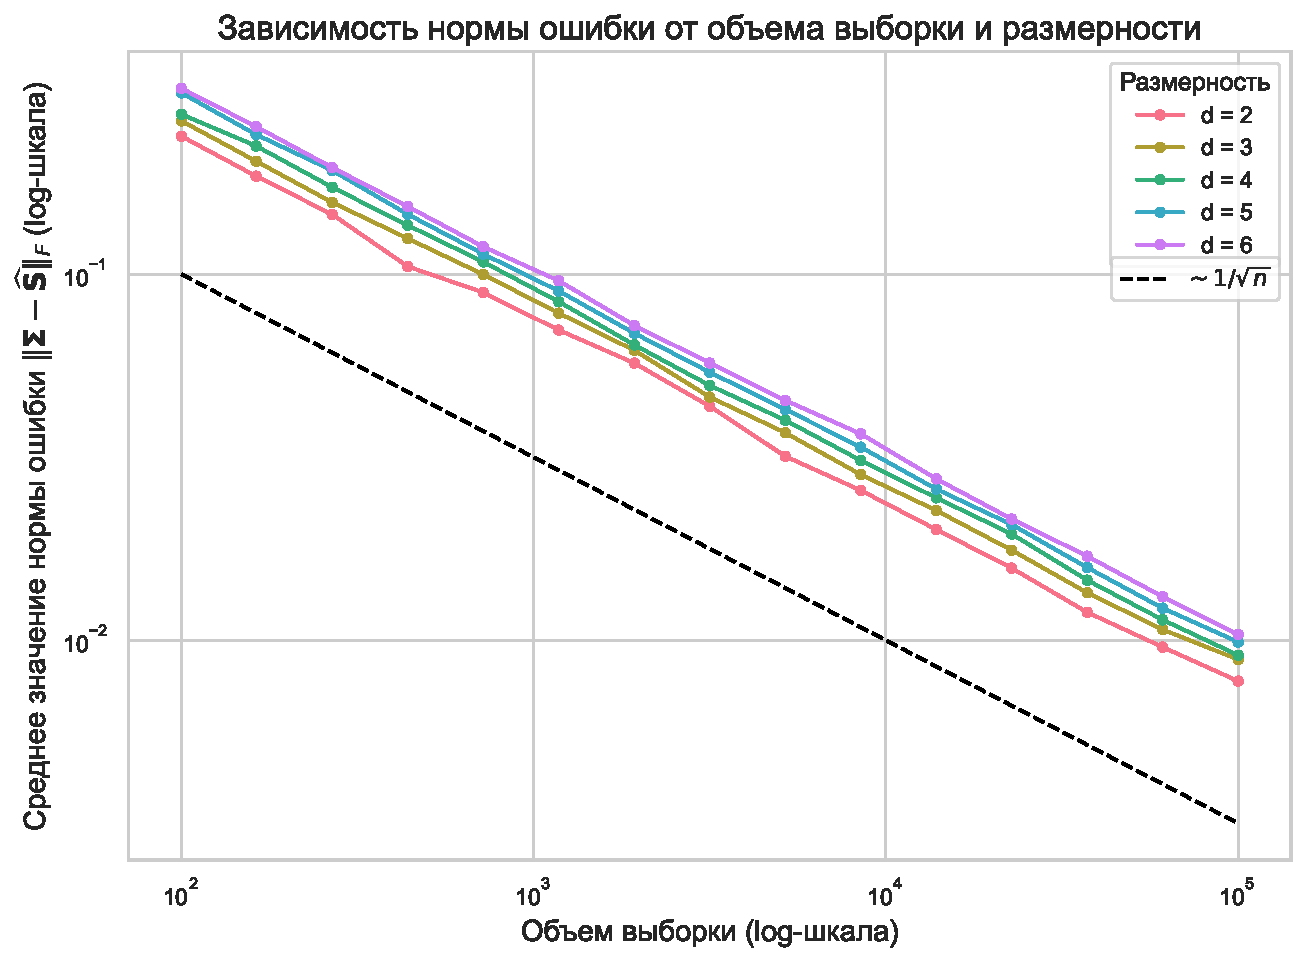
\includegraphics[width=0.95\textwidth]{covariance_consistency_v2.pdf}
    \caption{Зависимость средней нормы ошибки $\|\widehat{\mathbf{S}} - \mathbf{S}\|_F$ от объема выборки $n$ и размерности $d$.}
    \label{fig:consistency}
\end{figure}

\subsection*{Анализ робастности метода ARR-GK}

Во втором эксперименте оценивалась устойчивость метода к добавлению точки-выброса с определенным весом. Сравнение ARR-GK проводилось с классической выборочной ковариационной матрицей на выборке из нормального распределения ($d=3, n=1000$) с истиной ковариационной матрицей \eqref{eq:experimentmatrix} при наличии от 0\% до 25\% выбросов. Для каждой выборки выполнялось $200$ независимых моделирований и рассчитывалась средняя ошибка.

Во втором эксперименте исследовалась устойчивость метода ARR-GK к наличию выбросов. Сравнение проводилось с классической выборочной ковариационной матрицей на выборках из нормального распределения ($d=3$, $n=1000$) с ковариационной матрицей~\eqref{eq:experimentmatrix}.

Для моделирования выбросов часть наблюдений заменялась фиксированной точкой-выбросом, а доля таких наблюдений варьировалась от $0\%$ до $25\%$. Для каждого случая проводилось $200$ независимых моделирований, после чего вычислялась средняя ошибка оценки матрицы разброса.


% Во втором эксперименте исследовалась устойчивость алгоритма ARR-GK к наличию выбросов. Для сравнения рассматривалась классическая выборочная ковариационная матрица.

% Эксперимент проводился на выборках объема $n=1000$ из трехмерного нормального распределения с коррелированными координатами. После генерации выборки часть наблюдений заменялась фиксированной точкой-выбросом большого масштаба. Доля выбросов изменялась от $0\%$ до $25\%$. Для каждой выборки  выполнялось $200$ независимых моделирований.


\begin{figure}[h!]
    \centering
    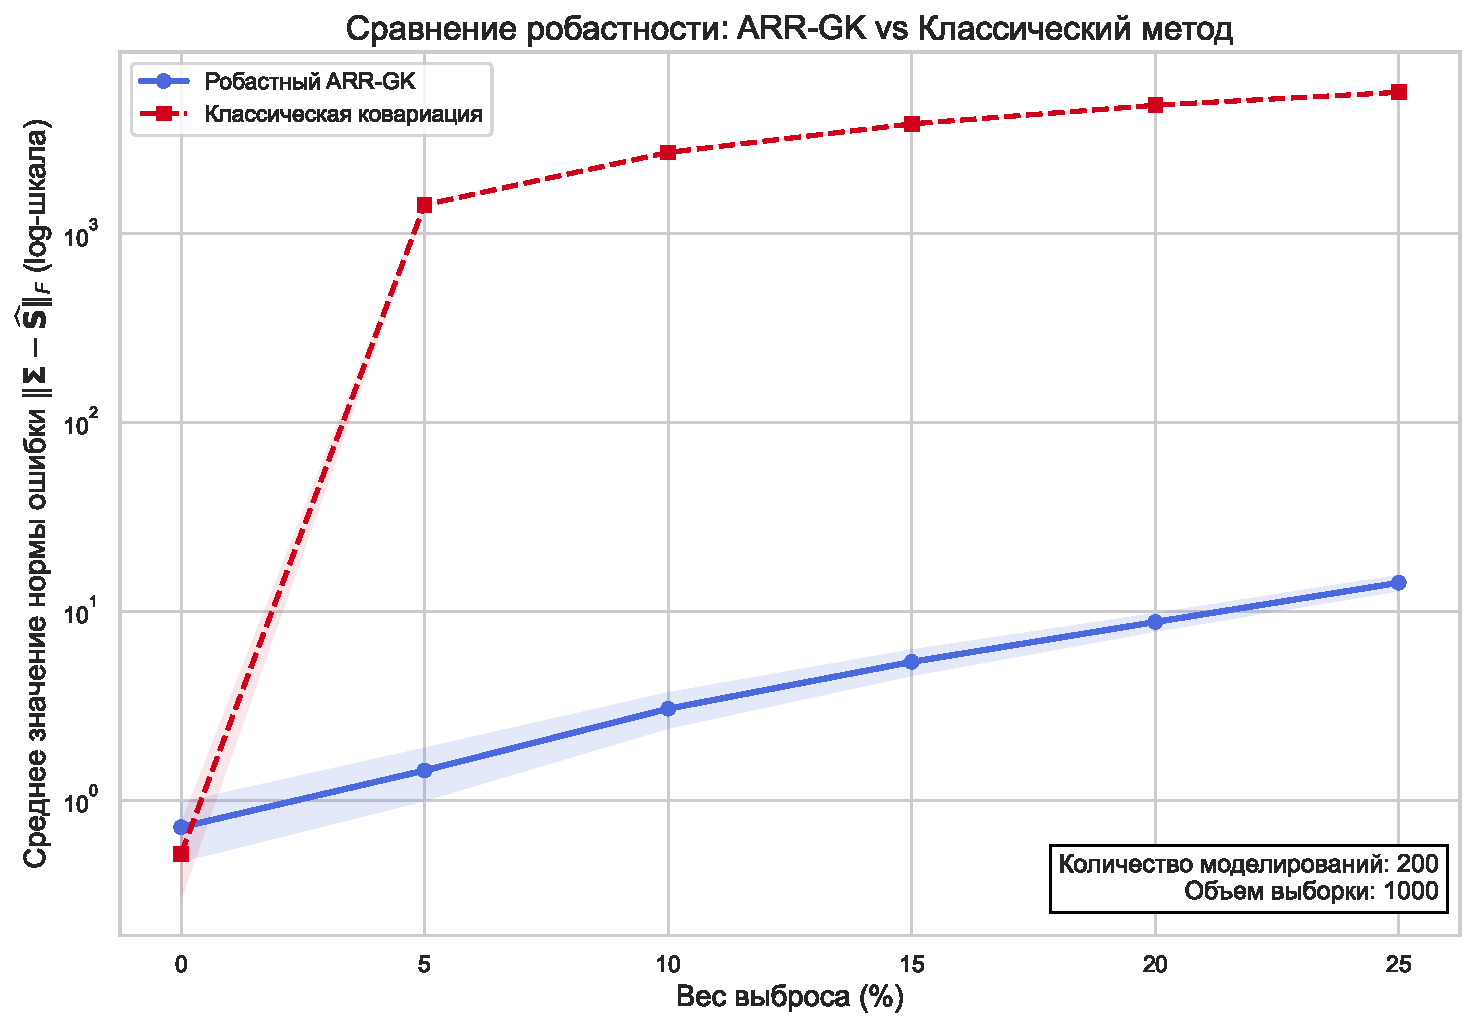
\includegraphics[width=0.9\textwidth]{robustness_comparison_log.pdf}
    \caption{Сравнение робастности ARR-GK и классической ковариационной матрицы при различном весе выбросов.}
    \label{fig:robustness}
\end{figure}

Результаты эксперимента представлены на Рисунке~\ref{fig:robustness}. Видно, что ошибка классической ковариационной матрицы резко возрастает уже при небольшом количестве выбросов. При добавлении $5\%$ выбросов значение ошибки увеличивается на несколько порядков, а дальнейшее увеличение доли выбросов приводит к еще большему ухудшению качества оценки.

В отличие от классического метода, алгоритм ARR-GK демонстрирует существенно более устойчивое поведение. Несмотря на постепенный рост ошибки при увеличении доли выбросов, изменение происходит значительно медленнее, а сама ошибка остается на сравнительно небольшом уровне даже при наличии большого числа выбросов.

Таким образом, проведённый эксперимент показывает, что алгоритм ARR-GK сохраняет устойчивость к выбросам значительно лучше классической выборочной ковариационной матрицы. При увеличении доли выбросов ошибка оценки возрастает существенно медленнее, что экспериментально подтверждает робастность предложенного алгоритма.

\subsection*{Сравнительный анализ ARR-GK с методами GK и F-MCD}

Заключительный эксперимент был направлен на сравнение ARR-GK с базовым методом Гнанадесикана-Кеттеринга (GK) и классическим робастным методом Fast-MCD в различных сценариях.

\textbf{Сравнение на выборке из нормального распределения}

\begin{figure}[h!]
    \centering
    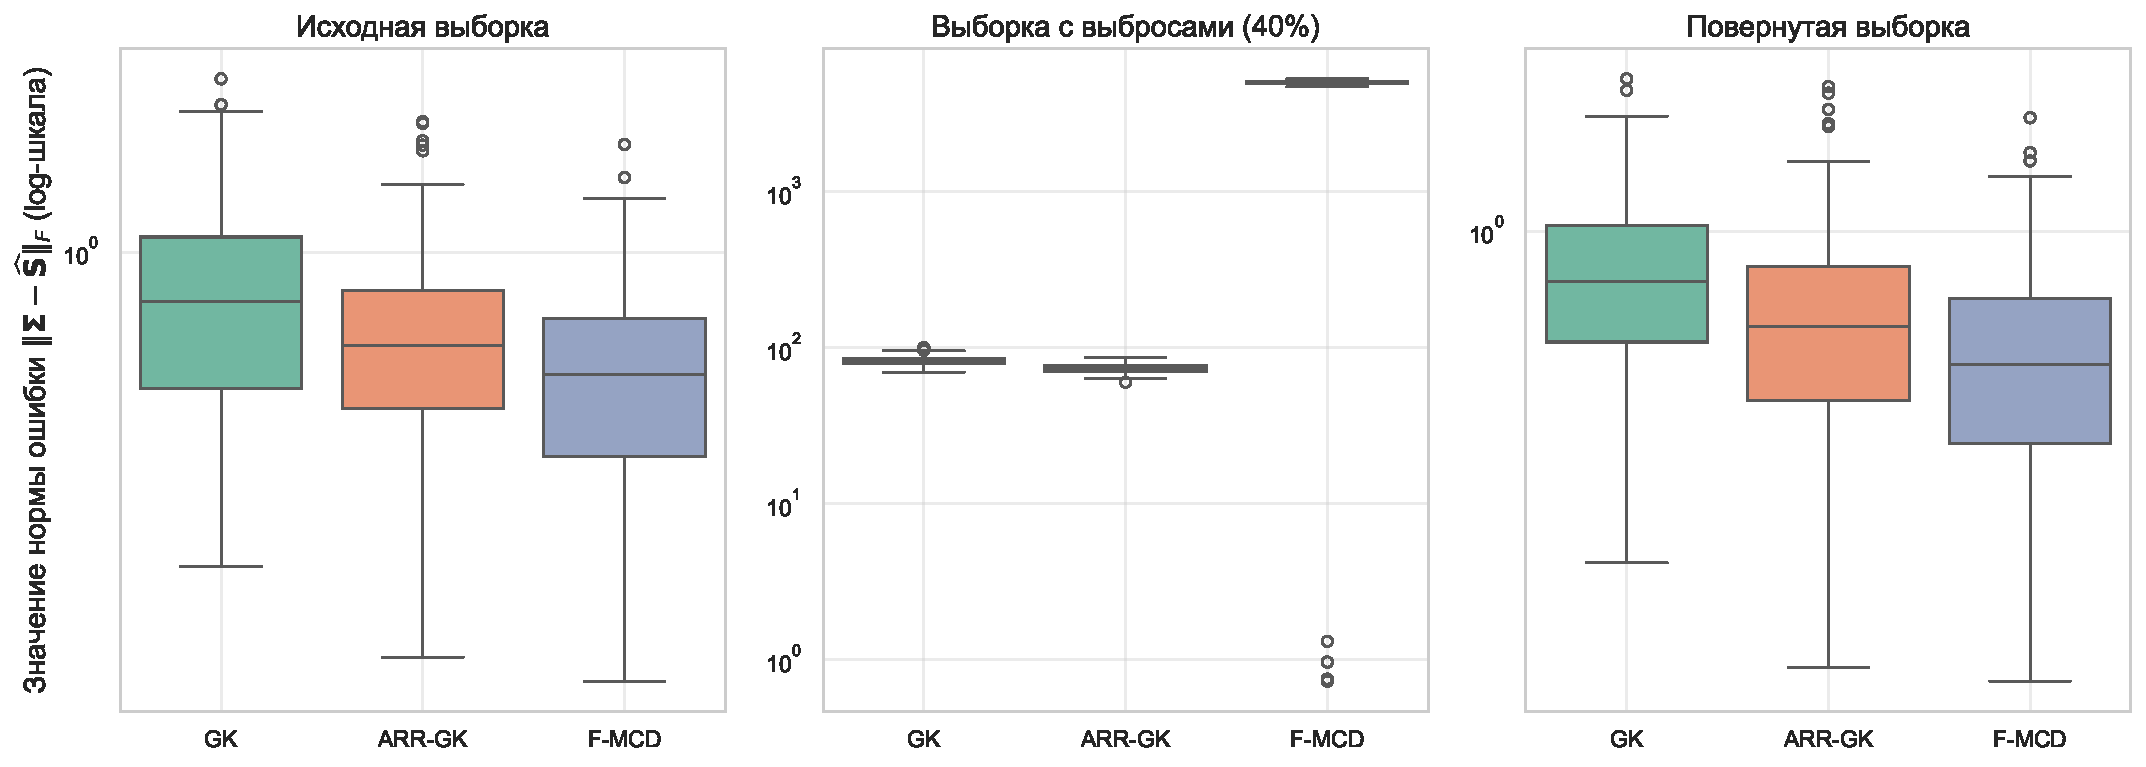
\includegraphics[width=1\textwidth]{comparison_GK_ARR_FMCD.pdf}
    \caption{Распределение нормы ошибки для алгоритмов GK, ARR-GK и F-MCD в различных условиях.}
    \label{fig:comparison_methods}
\end{figure}

На Рисунке~\ref{fig:comparison_methods} представлены результаты сравнения методов GK, ARR-GK и F-MCD для трех различных сценариев: исходной выборки, выборки с $40\%$ выбросов и повернутой выборки.
\begin{enumerate}
    \item \textbf{Исходная выборка:} Для исходной выборки все три метода демонстрируют сопоставимый уровень ошибки. При этом метод F-MCD показывает немного меньшую медианную ошибку и меньший разброс оценок по сравнению с GK и ARR-GK.\vspace{-2ex}
    \item \textbf{Выборка с выбросами (40\%):} В случае выборки с $40\%$ выбросов методы GK и ARR-GK сохраняют устойчивое поведение и дают близкие результаты, тогда как для метода F-MCD наблюдается существенное увеличение ошибки. Это связано с тем, что доля выбросов оказывается близкой к предельному уровню устойчивости метода MCD.\vspace{-2ex}
    \item \textbf{Повернутая выборка:} Для повернутой выборки метод GK демонстрирует увеличение разброса ошибок, тогда как ARR-GK сохраняет более стабильное поведение. При этом метод F-MCD снова показывает наименьшую медианную ошибку среди рассматриваемых алгоритмов. Из-за отсутствия выбросов и простой формы нормального распределения данный сценарий не выявляет особого преимущества ARR-GK перед базовым методом GK. Для того, чтобы продемонстрировать преимущество метода ARR-GK перед GK требуется произвести эксперимент с более сложной выборкой.
\end{enumerate}

Таким образом, результаты эксперимента показывают, что алгоритм ARR-GK позволяет уменьшить чувствительность метода GK к поворотам выборки, сохраняя при этом робастность при наличии большого числа выбросов.

\vspace{1.5ex}

\textbf{Сравнение на несимметричной выборке}

Чтобы показать, что алгоритм GK не устойчив относительно вращений, в отличие от ARR-GK, рассмотрим следующий пример. 

Промоделируем $n=1000$ случайных трехмерных векторов, компоненты которых являются независимыми реализациями экспоненциально распределенной случайной величины с параметром $\lambda=1$, центрированной таким образом, чтобы распределение имело нулевое математическое ожидание и единичную дисперсию.

Далее применим к выборке два линейных преобразования $\mathbf{U}_1$ и $\mathbf{U}_2$, причем $\mathbf{U}_2$ получается из $\mathbf{U}_1$ ортогональным преобразованием:
\begin{equation*}
\mathbf{U}_1 = \begin{pmatrix}
-0{,}707 & -0{,}707 & -1{,}000 \\
-0{,}060 & -1{,}944 & 0{,}467 \\
-2{,}631 & -0{,}161 & 1{,}025
\end{pmatrix}, \quad
\mathbf{U}_2 = \begin{pmatrix}
1{,}414 & 0{,}000 & 0{,}000 \\
0{,}672 & 1{,}884 & 0{,}000 \\
0{,}672 & 0{,}265 & 2{,}735
\end{pmatrix}.
\end{equation*}

Для полученных выборок были применены алгоритмы GK, ARR-GK и F-MCD. Результаты представлены на Рисунке~\ref{fig:comparison_methods_nonnorm}.

Из Рисунка~\ref{fig:comparison_methods_nonnorm} видно, что для исходной выборки методы GK и ARR-GK показывают сопоставимые результаты. Однако после поворота выборки ошибка метода GK существенно возрастает, тогда как качество оценки ARR-GK практически не изменяется. Это экспериментально подтверждает устойчивость предложенного алгоритма относительно вращений выборки.

При этом метод F-MCD в данном эксперименте показывает более высокую ошибку по сравнению с ARR-GK, что особенно заметно для несимметричного распределения.

\begin{figure}[h!]
    \centering
    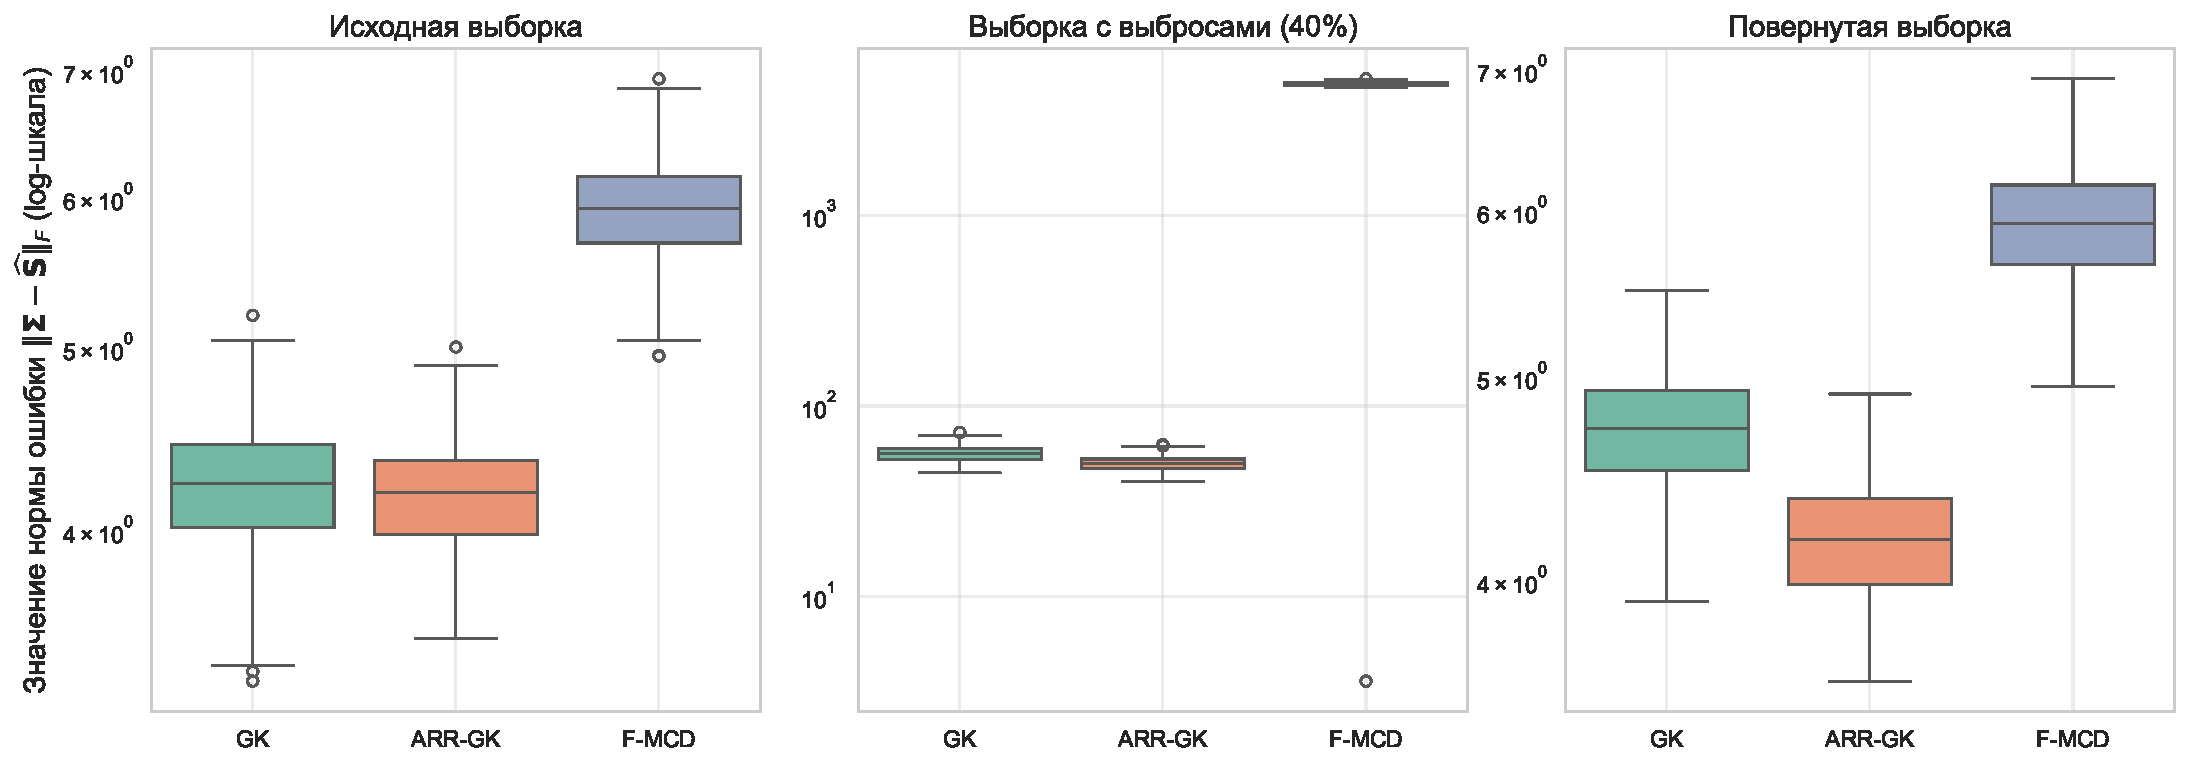
\includegraphics[width=1\textwidth]{comparison_GK_ARR_FMCD_nonnorm.pdf}
    \caption{Распределение нормы ошибки для алгоритмов GK, ARR-GK и F-MCD в различных условиях для исходной выборки (преобразование $\mathbf{U}_1$) и повернутой (преобразование $\mathbf{U}_2$).}
    \label{fig:comparison_methods_nonnorm}
\end{figure}

\vspace{1ex}

Таким образом, проведенные эксперименты показывают, что алгоритм ARR-GK сочетает вычислительную устойчивость метода GK с эквивариантностью относительно вращений. Кроме того, метод сохраняет робастность при наличии выбросов и демонстрирует более стабильное поведение по сравнению с классическим подходом GK на несимметричных распределениях.

\chapter{Заключение}

В рамках данной работы был проведён подробный анализ ранее предложенного стохастического алгоритма робастного оценивания многомерного параметра положения. Основное внимание было уделено исследованию теоретических свойств алгоритма, а также разработке модификаций, направленных на повышение точности и устойчивости оценки.

Была установлена важная теоретическая связь предложенного алгоритма с проекционной медианой и методом yamm. Показано, что получаемая алгоритмом оценка эквивалентна оценке по методу yamm, что позволяет перенести на неё известные теоретические свойства проекционной медианы, включая эквивариантность относительно вращений.

Проведено исследование эквивариантности алгоритма. Показано, что для ортогональных преобразований отклонение от эквивариантности оказывается близким к нулю, тогда как для более общих аффинных преобразований свойство аффинной эквивариантности не выполняется. При этом характер поведения алгоритма оказался сопоставим с геометрической медианой, которая являлась основным конкурирующим методом в рамках работы.

Для повышения устойчивости и точности оценки были предложены и исследованы несколько модификаций алгоритма. Рассматривались условия на минимальное число итераций, многократное выполнение критерия останова, усреднение последних итераций, экспоненциальное сглаживание, а также адаптивный выбор шага на основе метода AdaGrad. Наиболее устойчивые результаты были получены для модификаций, использующих экспоненциальное сглаживание и усреднение последних итераций. Проведённые численные эксперименты показали, что данные подходы позволяют существенно уменьшить разброс оценки и снизить влияние случайности, возникающей из-за стохастической природы алгоритма.

Кроме того, были исследованы специальные примеры, в которых базовый алгоритм не демонстрирует устойчивой сходимости. Рассматривались выборки в форме букв V и C, а также выборки, состоящие из вершин вложенных треугольников. Показано, что предложенные модификации позволяют добиться приближённой сходимости даже в подобных сложных случаях: траектории алгоритма концентрируются вблизи истинного параметра положения и образуют компактные области вместо хаотичного поведения базовой версии алгоритма.

Отдельное внимание было уделено исследованию поведения алгоритма на выборках различной природы. Проведены эксперименты для непрерывных и дискретных распределений, а также для выборок, заданных в выпуклых, невыпуклых и несвязных областях. Результаты показали, что предложенный алгоритм остаётся применимым и в случаях, не связанных с эллиптически контурированными распределениями, хотя теоретическое объяснение данного поведения требует дальнейшего исследования.

В работе также была рассмотрена задача робастного оценивания матрицы разброса. Предложен метод, основанный на использовании случайных направлений и робастных оценок масштаба вдоль проекций выборки. Было показано, что данный подход связан с формулой Гнанадесикана--Кеттеринга, однако позволяет по-новому интерпретировать задачу восстановления матрицы разброса через случайные проекции. Кроме того, рассмотрен альтернативный вычислительно устойчивый подход, позволяющий избежать проблем, связанных с плохой обусловленностью возникающих систем линейных уравнений.

Таким образом, в работе удалось не только исследовать свойства исходного стохастического алгоритма, но и предложить ряд его улучшений, существенно повышающих устойчивость и качество оценивания. Полученные результаты показывают перспективность подходов, основанных на случайных проекциях и робастных одномерных статистиках, для задач многомерного робастного анализа данных.

В качестве направлений дальнейших исследований представляют интерес теоретическое изучение сходимости алгоритма для неэллиптических распределений, исследование аффинно-эквивариантных модификаций метода, а также дальнейшее развитие подходов к робастному оцениванию матрицы разброса.



% В рамках работы был проведен более подробный анализ предложенного ранее робастного алгоритма для оценки многомерного параметра положения. Особое внимание уделено его модификациям, направленным на повышение устойчивости и точности. Одной из ключевых доработок стало добавление экспоненциального сглаживания с усреднением последних итераций, что позволило значительно снизить ошибку оценки и повысить стабильность алгоритма.

% % Важным результатом стало эмпирическое исследование эквивариантности алгоритма. Для ортогональных преобразований отклонение от эквивариантности оказалось близким к нулю, а для диагональных матриц и матриц сдвига медианная ошибка не превышала $0,1$, что сопоставимо с точностью геометрической медианы. Однако эквивариантности для произвольной матрицы преобразования не наблюдается.

% Была получена важная теоретическая связь оценки, полученной предложенным алгоритмом, с оценкой проекционной медианы и оценки по методу yamm. Показана эквивалентность полученной оценки с оценкой по методу yamm, из чего сделан вывод о совпадении теоретических свойств оценки.

% Помимо этого, были рассмотрены случаи, когда алгоритм не сходится, которые демонстрируют, что некоторые специально подобранные примеры являются сложными задачами для предложенного алгоритма. Однако для таких проблемных случаев (выборки в форме V, C, вершин треугольников) предложенная модификация с экспоненциальным сглаживанием и усреднением обеспечивает приближенную сходимость, когда оценки образуют компактное облако вблизи истинного значения.

% Кроме того, была проведена эмпирическая оценка точности алгоритма для различных типов областей и распределений, показавшая его применимость для распределений, не являющихся эллиптически контурированными. Однако теоретически пока сложно доказать, почему предложенный алгоритм в данных случаях сходится к истинному значению параметра положения.

% Дополнительно была разработана робастная оценка матрицы разброса, что стало важным шагом для полного описания многомерных данных. Было проведено улучшение методов оценки матриц разброса. Показано, что предложенная оценка имеет связь с ранее опубликованной оценкой, которая, однако, не устойчива относительно вращений данных. Приведен новый метод, который устраняет недостатки ранее предложенных оценок.

% Также рассмотрены методы улучшения сходимости последовательности при оценивании параметра положения. Разность между двумя соседними оценками в последовательности была интепретирована, как направление поиска медианы, после чего, помимо экспоненциального сглаживания, удалось рассмотреть модификацию для улучшения сходимости AdaGrad, позаимствованную из метода стохастического градиента.

% На основе проделанной работы определены перспективные направления для дальнейших исследований.


 \bibliographystyle{ugost2008}
  \bibliography{bibliography}
  %\addcontentsline{toc}{section}{Список литературы}

\end{document}
